% gcodepreview.tex
% Author: William F. Adams (willadams at aol dot com)
% Copyright 2021--24 William F. Adams
%
% This work may be distributed and/or modified under the
% conditions of the GNU LESSER GENERAL PUBLIC LICENSE
% Version 2.1, February 1999
%
% This work consists of the files listed in the README file.
%
% 
% 
\documentclass{ltxdoc}
%https://tex.stackexchange.com/questions/722886/how-to-write-out-multiple-text-files-from-multiple-instances-of-latex-environmen
\usepackage{literati}
\usepackage[paper=legalpaper,left=1.75in,right=0.75in,top=1in,bottom=1in]{geometry}

\begin{document}

%\DoNotIndex{\bullet}

%\changes{v0.71}{2024/11/11}{Restore G2/G3 arcs, roundover tooling}
\def\fileversion{v0.71} \def\filedate{2024/11/29}

%\changes{v0.7}{2024/11/11}{Python re-write}
%\def\fileversion{v0.7} \def\filedate{2024/11/11}

%\changes{v0.61}{2024/09/08}{modules and tests}
%\def\fileversion{v0.61} \def\filedate{2024/09/08}

%\changes{v0.6}{2024/08/30}{modules and setupstock}
%\def\fileversion{v0.6} \def\filedate{2024/08/30}

%\changes{v0.5}{2024/08/10}{DXFs and images}
%\def\fileversion{v0.5} \def\filedate{2024/08/10}

%\changes{v0.4}{2024/07/28}{Literary re-write}
%\def\fileversion{v0.4} \def\filedate{2024/07/28}

%\changes{v0.3}{2024/07/01}{Curves and roundover tooling}
%\def\fileversion{v0.3} \def\filedate{2024/07/01}

%\changes{v0.2}{2024/04/12}{Initial conversion to DTX}
%\def\dtxfile{gcodepreview.dtx}

\title{The gcodepreview OpenSCAD library\thanks{This
        file (\texttt{\jobname}) has version number \fileversion, last revised
        \filedate.}}

\author{%
Author: William F. Adams\\
\texttt{willadams at aol dot com}
}
\date{\filedate}
\maketitle
\begin{abstract}
\noindent The gcodepreview library allows using OpenPythonSCAD to move a tool in lines 
and arcs and output dxf and G-code files so as to work as a CAD/\allowbreak CAM program 
for CNC.
\end{abstract}
%\enlargethispage{\baselineskip}
\tableofcontents

\clearpage
\section{readme.md}

\begin{readme}
# gcodepreview

OpenPythonSCAD library for moving a tool in lines and arcs so as to model how a part would be cut using G-Code, so as to allow OpenPythonSCAD to function as a compleat CAD/CAM solution for subtractive 3-axis CNC (mills and routers) by writing out G-code in addition to 3D modeling (in some cases toolpaths which would not normally be feasible), and to write out DXF files which may be imported into a traditional CAM program to create toolpaths.

![OpenSCAD Cut Joinery Module](https://raw.githubusercontent.com/WillAdams/gcodepreview/main/gcodepreview_unittests.png?raw=true)

Updated to make use of Python in OpenSCAD:[^rapcad]

[^rapcad]: Previous versions had used RapCAD, so as to take advantage of the writeln command, which has since been re-written in Python.

https://pythonscad.org/ (previously this was http://www.guenther-sohler.net/openscad/ )

A BlockSCAD file for the initial version of the 
main modules is available at:

https://www.blockscad3d.com/community/projects/1244473

The project is discussed at:

https://forum.makerforums.info/t/g-code-preview-using-openscad-rapcad/85729 

and

https://forum.makerforums.info/t/openscad-and-python-looking-to-finally-be-resolved/88171

and

https://willadams.gitbook.io/design-into-3d/programming

Since it is now programmed using Literate Programming (initially a .dtx, now a .tex file) there is a PDF: https://github.com/WillAdams/gcodepreview/blob/main/gcodepreview.pdf which includes all of the source code with formatted commentary.

The files for this library are:

 - gcodepreview.py (gcpy) --- the Python functions and variables
 - pygcodepreview.scad (pyscad) --- the Python functions wrapped in OpenSCAD
 - gcodepreview.scad (gcpscad) --- OpenSCAD modules and variables
 - gcodepreview_template.scad (gcptmpl) --- example file
 - cut2Dshapes.scad (cut2D) --- code for cutting 2D shapes 

If using from OpenPythonSCAD, place the files in C:\Users\\\~\Documents\OpenSCAD\libraries and call as:[^libraries]

[^libraries]: C:\Users\\\~\Documents\RapCAD\libraries is deprecated since RapCAD is no longer needed since Python is now used for writing out files)

    use <gcodepreview.py>;
    use <pygcodepreview.scad>;
    include <gcodepreview.scad>;

Note that it is necessary to use the first two files (this allows loading the Python commands and then wrapping them in OpenSCAD commands) and then include the last file (which allows using OpenSCAD variables to selectively implement the Python commands via their being wrapped in OpenSCAD modules) and define variables which match the project and then use commands such as:

    opengcodefile(Gcode_filename);
    opendxffile(DXF_filename);
    
    difference() {
        setupstock(stockXwidth, stockYheight, stockZthickness, zeroheight, stockzero);
    
    movetosafez();
    
    toolchange(squaretoolnum,speed * square_ratio);
    
    begintoolpath(0,0,0.25);
    beginpolyline(0,0,0.25);

    cutoneaxis_setfeed("Z",-1,plunge*square_ratio);
    addpolyline(stockXwidth/2,stockYheight/2,-stockZthickness);
    
    cutwithfeed(stockXwidth/2,stockYheight/2,-stockZthickness,feed);
    
    endtoolpath();
    endpolyline();
    
    }
    
    closegcodefile();
    closedxffile();

which makes a G-code file:

![OpenSCAD template G-code file](https://raw.githubusercontent.com/WillAdams/gcodepreview/main/gcodepreview_template.png?raw=true)

but one which could only be sent to a machine so as to cut only the softest and most yielding of materials since it makes a single full-depth pass, and of which has a matching DXF which may be imported into a CAM tool --- but which it is not directly possible to assign a toolpath in readily available CAM tools (since it varies in depth from beginning-to-end). 

Importing this DXF and actually cutting it is discussed at:

https://forum.makerforums.info/t/rewriting-gcodepreview-with-python/88617/14

Alternately, gcodepreview.py may be placed in a Python library location and used directly from Python --- note that it may become possible to use it from a "normal" Python when generating only DXFs.

Tool numbers match those of tooling sold by Carbide 3D (ob. discl., I work for them). 

Comments are included in the G-code to match those expected by CutViewer.

A complete example file is: gcodepreview_template.scad Note that a Python template has since been developed as well, allowing usage without OpenSCAD code, and another example is openscad_gcodepreview_cutjoinery.tres.scad which is made from an OpenSCAD Graph Editor file:

![OpenSCAD Graph Editor Cut Joinery File](https://raw.githubusercontent.com/WillAdams/gcodepreview/main/OSGE_cutjoinery.png?raw=true)

Version 0.1 supports setting up stock, origin, rapid positioning, making cuts, and writing out matching G-code, and creating a DXF with polylines.

Added features since initial upload:

 - endpolyline(); --- this command allows ending one polyline so as to allow multiple lines in a DXF
 - separate dxf files are written out for each tool where tool is ball/square/V and small/large (10/31/23)
 - re-writing as a Literate Program using the LaTeX package docmfp (begun 4/12/24) 
 - support for additional tooling shapes such as dovetail and keyhole tools

Version 0.2 adds support for arcs 

 - DXF: support for arcs (which may be used to make circles) (6/1/24)
 - Specialty toolpaths such as Keyhole which may be used for dovetail as well as keyhole cutters

Version 0.3 

 - Support for curves along the 3rd dimension
 - support for roundover tooling
 
Version 0.4

 - Rewrite using literati documentclass, suppression of SVG code
 - dxfrectangle (without G-code support)

Version 0.5

 - more shapes
 - consolidate rectangles, arcs, and circles in gcodepreview.scad
 
Version 0.6

 - notes on modules
 - change file for setupstock

Version 0.61

 - validate all code so that it runs without errors from sample
 - NEW: Note that this version is archived as gcodepreview-openscad_0_6.tex and the matching PDF is available as well
 
 Version 0.7
 
  - re-write completely in Python --- note that it is possible to use from within OpenPythonSCAD and an OpenSCAD wrapper is not functional at this time --- note that the OpenSCAD wrapper will need to be rewritten

Possible future improvements:

 - rewrite OpenSCAD wrapper
 - support for additional tooling shapes (bowl bits with flat bottom, tapered ball nose, lollipop cutters)
 - create a single line font for use where text is wanted

Note for G-code generation that it is up to the user to implement Depth per Pass so as to not take a single full-depth pass. Working from a DXF of course allows one to off-load such considerations to a specialized CAM tool.

Deprecated feature:

 - exporting SVGs --- coordinate system differences between OpenSCAD/DXFs and SVGs would require managing the inversion of the coordinate system (using METAPOST, which shares the same orientation and which can write out SVGs may be used for future versions)

\end{readme}

\clearpage
\section{gcodepreview}

This library for OpenPythonSCAD works by using Python code as a back-end so as to persistently store and access variables, and to write out files while both modeling the motion of a 3-axis CNC machine and if desired, writing out DXF and/or G-code files (as opposed to the normal technique of rendering to a 3D model and writing out an STL or STEP or other model format). There are multiple modes for this, doing so requires up to three files:

\begin{itemize}
\item A Python file: gcodepreview.py (\texttt{gcpy}) --- this has variables in the 
      traditional sense which may be used for tracking machine position and so forth. 
      Note that where it is placed/loaded from will depend on whether it is imported into
      a Python file:\\
      \verb|import gcodepreview_standalone as gcp|\\ 
      or used in an OpenSCAD file:\\
      \verb|use <gcodepreview.py>|\\
      with additional OpenSCAD modules which allow accessing it
\item An OpenSCAD file: pygcodepreview.scad (\texttt{pyscad}) --- which wraps the Python code 
      in OpenSCAD (note that it too is included by \verb|use <pygcodepreview.scad>|)
\item An OpenSCAD file: gcodepreview.scad (\texttt{gcpscad}) --- which uses the other two files 
      and which is \texttt{include}d allowing it to access OpenSCAD variables for branching   
\end{itemize}

\noindent Note that this architecture requires that many OpenSCAD modules are essentially 
``Dispatchers'' which pass information from one aspect of the environment to another.

\subsection{gcodepreviewtemplate}

The various commands are shown all together in templates so as to provide examples of usage, and to ensure that the various files are used/included as necessary, all variables are set up with the correct names, and that files are opened before being written to, and that each is closed at the end. 

Note that while the template files seem overly verbose, they specifically incorporate variables for each tool shape, possibly in two different sizes, and a feed rate parameter or ratio for each, which may be used (by setting a tool \#) or ignored (by leaving the variable at zero (0).

It should be that this section is all the documentation which some users will need (and arguably is still too much). The balance of the document after this section shows all the code and implementation details.

%Creating a template from memory, the file should be something like:
%
%List of all tools
%chipload for each tool
%Depth per Pass for each tool
%scaling factor for chipload to arrive at feeds and speeds
%Booleans for generateDXF/Gcode, 3D Preview, assembly or parts or drop-down list of parts, &c.
%
%setupstock --- should this open gcode/dxf files as well?
%
%toolchange to first tool
%
%Rapid to location of first cut
%cutline/cutarc --- iterate as needed
%Rapid to safe height
%
%Program END --- should close gcode/DXF files and include rapid to safe height and rapid to back

\subsubsection{gcodepreviewtemplate.scad}

\lstset{firstnumber=1}%\thegcptmpl}
\begin{writecode}{w}{gcodepreviewtemplate.scad}{scad}
//!OpenSCAD

use <gcodepreview.py>;
use <pygcodepreview.scad>;
include <gcodepreview.scad>;

$fa = 2;
$fs = 0.125;

/* [Stock] */
stockXwidth = 219;
/* [Stock] */
stockYheight = 150;
/* [Stock] */
stockZthickness = 8.35;
/* [Stock] */
zeroheight = "Top"; // [Top, Bottom]
/* [Stock] */
stockzero = "Center"; // [Lower-Left, Center-Left, Top-Left, Center]
/* [Stock] */
retractheight = 9;

/* [Export] */
Base_filename = "export"; 
/* [Export] */
generatedxf = true; 
/* [Export] */
generategcode = true; 
///* [Export] */
//generatesvg = false; 

/* [CAM] */
toolradius = 1.5875;
/* [CAM] */
large_square_tool_num = 0; // [0:0,112:112,102:102,201:201]
/* [CAM] */
small_square_tool_num = 102; // [0:0,122:122,112:112,102:102]
/* [CAM] */
large_ball_tool_num = 0; // [0:0,111:111,101:101,202:202]
/* [CAM] */
small_ball_tool_num = 0; // [0:0,121:121,111:111,101:101]
/* [CAM] */
large_V_tool_num = 0; // [0:0,301:301,690:690]
/* [CAM] */
small_V_tool_num = 0; // [0:0,390:390,301:301]
/* [CAM] */
DT_tool_num = 0; // [0:0,814:814]
/* [CAM] */
KH_tool_num = 0; // [0:0,374:374,375:375,376:376,378]
/* [CAM] */
Roundover_tool_num = 0; // [56142:56142, 56125:56125, 1570:1570]
/* [CAM] */
MISC_tool_num = 0; // 

/* [Feeds and Speeds] */
plunge = 100;
/* [Feeds and Speeds] */
feed = 400;
/* [Feeds and Speeds] */
speed = 16000;
/* [Feeds and Speeds] */
small_square_ratio = 0.75; // [0.25:2]
/* [Feeds and Speeds] */
large_ball_ratio = 1.0; // [0.25:2]
/* [Feeds and Speeds] */
small_ball_ratio = 0.75; // [0.25:2]
/* [Feeds and Speeds] */
large_V_ratio = 0.875; // [0.25:2]
/* [Feeds and Speeds] */
small_V_ratio = 0.625; // [0.25:2]
/* [Feeds and Speeds] */
DT_ratio = 0.75; // [0.25:2]
/* [Feeds and Speeds] */
KH_ratio = 0.75; // [0.25:2]
/* [Feeds and Speeds] */
RO_ratio = 0.5; // [0.25:2]
/* [Feeds and Speeds] */
MISC_ratio = 0.5; // [0.25:2]

filename_gcode = str(Base_filename, ".nc");
filename_dxf = str(Base_filename);

opengcodefile(filename_gcode);
opendxffile(filename_dxf);

difference() {
setupstock(stockXwidth, stockYheight, stockZthickness, zeroheight, stockzero);

movetosafez();

toolchange(small_square_tool_num,speed * small_square_ratio);

begintoolpath(0,0,0.25);

cutoneaxis_setfeed("Z",0,plunge*small_square_ratio);

cutwithfeed(stockXwidth/2,stockYheight/2,-stockZthickness,feed);
dxfline(getxpos(),getypos(),stockXwidth/2,stockYheight/2, small_square_tool_num);

endtoolpath();
rapid(-(stockXwidth/4-stockYheight/16),stockYheight/4,0);
cutoneaxis_setfeed("Z",-stockZthickness,plunge*small_square_ratio);

cutarcNECCdxf(-stockXwidth/4, stockYheight/4+stockYheight/16, -stockZthickness, -stockXwidth/4, stockYheight/4, stockYheight/16, small_square_tool_num);
cutarcNWCCdxf(-(stockXwidth/4+stockYheight/16), stockYheight/4, -stockZthickness, -stockXwidth/4, stockYheight/4, stockYheight/16, small_square_tool_num);
cutarcSWCCdxf(-stockXwidth/4, stockYheight/4-stockYheight/16, -stockZthickness, -stockXwidth/4, stockYheight/4, stockYheight/16, small_square_tool_num);
cutarcSECCdxf(-(stockXwidth/4-stockYheight/16), stockYheight/4, -stockZthickness, -stockXwidth/4, stockYheight/4, stockYheight/16, small_square_tool_num);

rapid(getxpos(),getypos(),stockZthickness);
toolchange(KH_tool_num,speed * KH_ratio);
rapid(-stockXwidth/8,-stockYheight/4,0);

cutkeyhole_toolpath((stockZthickness), (stockZthickness), "N", stockYheight/8, KH_tool_num);
rapid(getxpos(),getypos(),stockZthickness);
rapid(-stockXwidth/4,-stockYheight/4,0);
cutkeyhole_toolpath((stockZthickness), (stockZthickness), "S", stockYheight/8, KH_tool_num);
rapid(getxpos(),getypos(),stockZthickness);
rapid(-stockXwidth/4,-stockYheight/8,0);
cutkeyhole_toolpath((stockZthickness), (stockZthickness), "E", stockYheight/8, KH_tool_num);
rapid(getxpos(),getypos(),stockZthickness);
rapid(-stockXwidth/8,-stockYheight/8*3,0);
cutkeyhole_toolpath((stockZthickness), (stockZthickness), "W", stockYheight/8, KH_tool_num);

rapid(getxpos(),getypos(),stockZthickness);
toolchange(DT_tool_num,speed * DT_ratio);
rapid(0,-(stockYheight/2+tool_diameter(DT_tool_num,0)),0);

cutoneaxis_setfeed("Z",-stockZthickness,plunge*DT_ratio);
cutwithfeed(0,-(stockYheight/4),-stockZthickness,feed*DT_ratio);
rapid(0,-(stockYheight/2+tool_diameter(DT_tool_num,0)),-stockZthickness);

rapid(getxpos(),getypos(),stockZthickness);
toolchange(Roundover_tool_num, speed * RO_ratio);
rapid(-(stockXwidth/2),-(stockYheight/2),0);
cutoneaxis_setfeed("Z",-4.509,plunge*RO_ratio);

cutroundovertool(-(stockXwidth/2++0.507/2), -(stockYheight/2+0.507/2), -4.509, stockXwidth/2+0.507/2, -(stockYheight/2+0.507/2), -4.509, 0.507/2, 4.509);

cutroundover(stockXwidth/2+0.507/2, -(stockYheight/2+0.507/2), -4.509, stockXwidth/2+0.507/2, stockYheight/2+0.507/2, -4.509, 1570);
cutroundover(stockXwidth/2+0.507/2, stockYheight/2+0.507/2, -4.509, -(stockXwidth/2+0.507/2), stockYheight/2+0.507/2, -4.509, 1570);
cutroundover(-(stockXwidth/2+0.507/2), stockYheight/2+0.507/2, -4.509, -(stockXwidth/2+0.507/2), -(stockYheight/2+0.507/2), -4.509, 1570);

//for (i = [0 : abs(1) : 80]) {
//  cutwithfeed(stockXwidth/4,-stockYheight/4,-stockZthickness/4,feed);
//  cutwithfeed(stockXwidth/8+(stockXwidth/256*i),-stockYheight/2,-stockZthickness*3/4,feed);
//  }

hull(){
  cutwithfeed(stockXwidth/4,-stockYheight/4,-stockZthickness/4,feed);
  cutwithfeed(stockXwidth/8,-stockYheight/2,-stockZthickness*3/4,feed);
  cutwithfeed(stockXwidth/8+(stockXwidth*0.3125),-stockYheight/2,-stockZthickness*3/4,feed);
  }
}

closegcodefile();
closedxffile();
\end{writecode}
\addtocounter{gcptmpl}{157}

%Note that the line:
%
%\begin{verbatim}
%toolchange(small_square_tool_num,speed * square_ratio);
%\end{verbatim}
%
%\noindent may be commented out --- whether or no it is actually necessary will need to be 
%decided upon.

\begin{samepage}
Which cuts as:

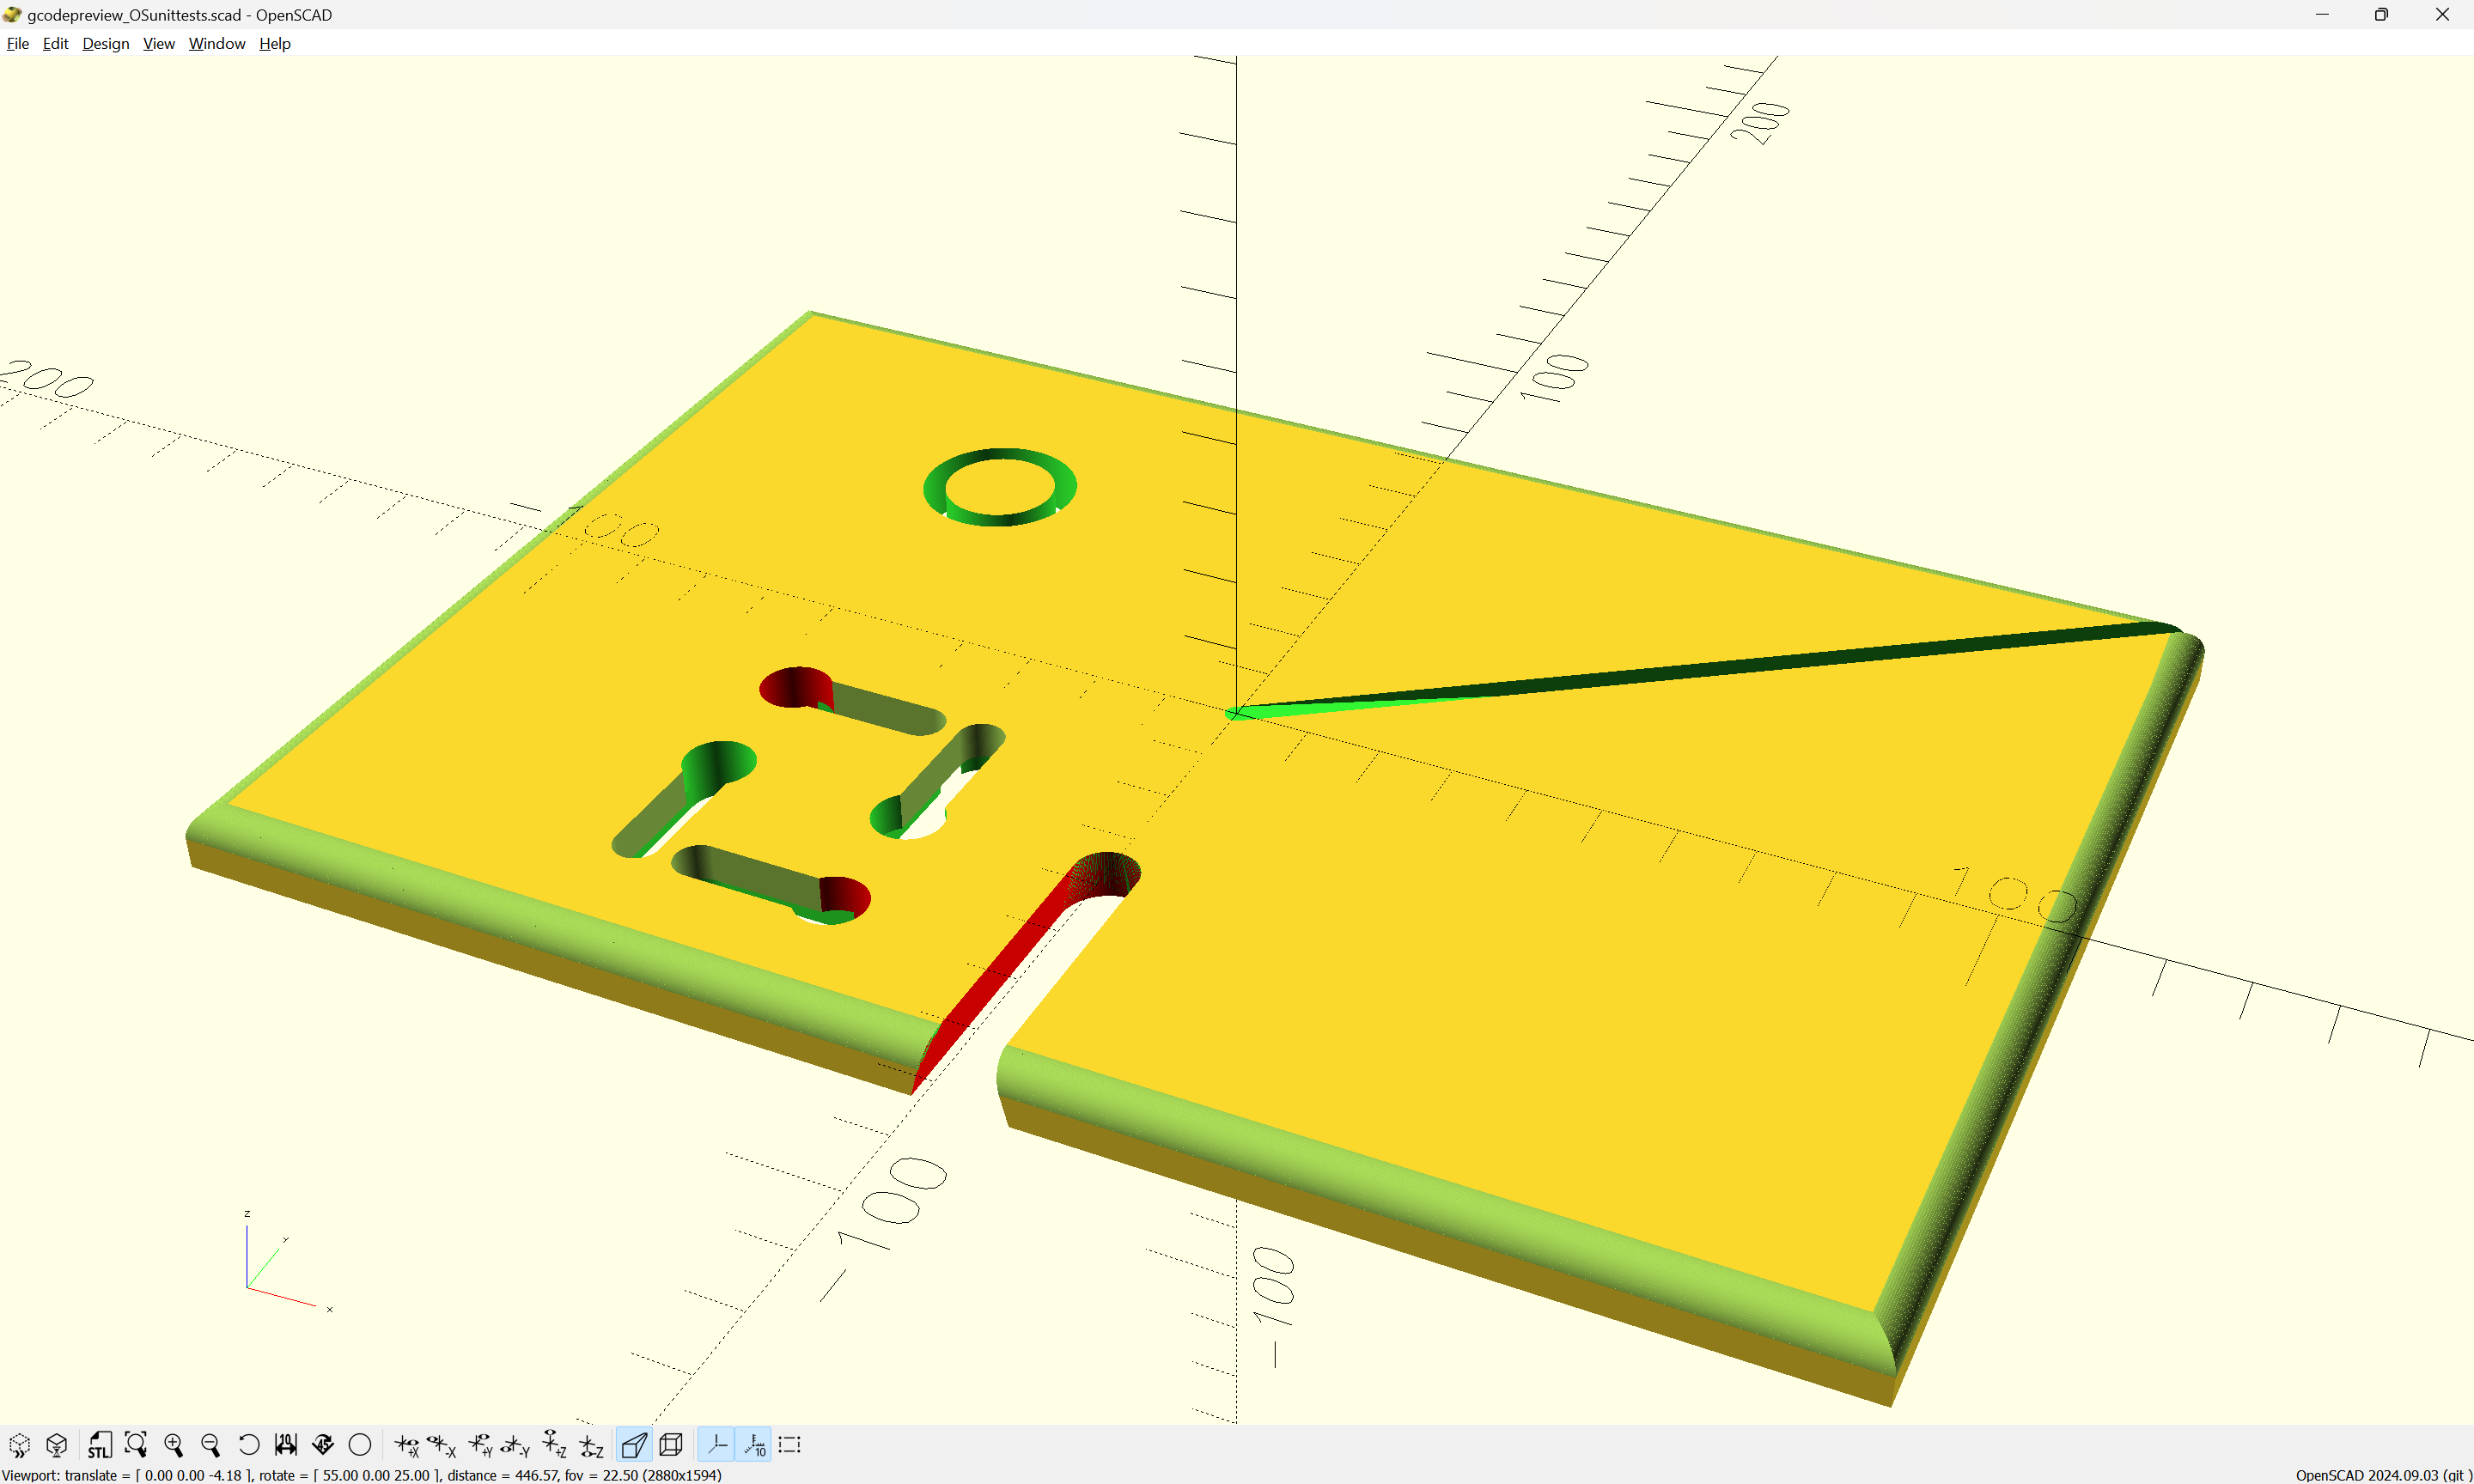
\includegraphics[width=\linewidth]{C:/Users/willa/OneDrive/Documents/GitHub/gcodepreview/gcodepreview_unittests.png}
\end{samepage}

Some comments on the template:

\begin{itemize}
\item minimal --- it is intended as a framework for a minimal working example (\textsc{mwe}) --- 
                  it should be possible to comment out unused portions and so arrive at code which 
                  tests any aspect of this project
\item compleat --- a quite wide variety of tools are listed (and probably more will be
                   added in the future), but pre-defining them and having these ``hooks'' seems
                   the easiest (non-object-oriented) mechanism to handle everything
\item shortcuts --- as the last example shows, while in real life it is necessary to make many 
                    passes with a tool, an expedient shortcut is to forgo the \verb|loop| 
                    operation and just use a \verb|hull()| operation
\end{itemize}

Further features will be added to the template, and the main image updated to reflect the capabilities of the system.


\subsubsection{gcodepreviewtemplate.py}
           
Note that with the v0.7 re-write, it is possible to directly use the underlying Python code directly.

\lstset{firstnumber=1}%\thegcptmplpy}
\begin{writecode}{w}{gcodepreviewtemplate.py}{python}
#!/usr/bin/env python

import sys

try:
    if 'gcodepreview' in sys.modules:
        del sys.modules['gcodepreview']
except AttributeError:
    pass

from gcodepreview import *

fa = 2
fs = 0.125

# [Export] */
Base_filename = "aexport"
# [Export] */
generatedxf = True
# [Export] */
generategcode = True

# [Stock] */
stockXwidth = 220
# [Stock] */
stockYheight = 150
# [Stock] */
stockZthickness = 8.35
# [Stock] */
zeroheight = "Top" # [Top, Bottom]
# [Stock] */
stockzero = "Center" # [Lower-Left, Center-Left, Top-Left, Center]
# [Stock] */
retractheight = 9

# [CAM] */
toolradius = 1.5875
# [CAM] */
large_square_tool_num = 201 # [0:0,112:112,102:102,201:201]
# [CAM] */
small_square_tool_num = 102 # [0:0,122:122,112:112,102:102]
# [CAM] */
large_ball_tool_num = 202 # [0:0,111:111,101:101,202:202]
# [CAM] */
small_ball_tool_num = 101 # [0:0,121:121,111:111,101:101]
# [CAM] */
large_V_tool_num = 301 # [0:0,301:301,690:690]
# [CAM] */
small_V_tool_num = 390 # [0:0,390:390,301:301]
# [CAM] */
DT_tool_num = 814 # [0:0,814:814]
# [CAM] */
KH_tool_num = 374 # [0:0,374:374,375:375,376:376,378]
# [CAM] */
Roundover_tool_num = 56142 # [56142:56142, 56125:56125, 1570:1570]
# [CAM] */
MISC_tool_num = 0 #

# [Feeds and Speeds] */
plunge = 100
# [Feeds and Speeds] */
feed = 400
# [Feeds and Speeds] */
speed = 16000
# [Feeds and Speeds] */
small_square_ratio = 0.75 # [0.25:2]
# [Feeds and Speeds] */
large_ball_ratio = 1.0 # [0.25:2]
# [Feeds and Speeds] */
small_ball_ratio = 0.75 # [0.25:2]
# [Feeds and Speeds] */
large_V_ratio = 0.875 # [0.25:2]
# [Feeds and Speeds] */
small_V_ratio = 0.625 # [0.25:2]
# [Feeds and Speeds] */
DT_ratio = 0.75 # [0.25:2]
# [Feeds and Speeds] */
KH_ratio = 0.75 # [0.25:2]
# [Feeds and Speeds] */
RO_ratio = 0.5 # [0.25:2]
# [Feeds and Speeds] */
MISC_ratio = 0.5 # [0.25:2]

gcp = gcodepreview(True, #generatescad
                   True, #generategcode
                   True, #generatedxf
                   )

gcp.opengcodefile(Base_filename)
gcp.opendxffile(Base_filename)
gcp.opendxffiles(Base_filename,
                 large_square_tool_num, 
                 small_square_tool_num, 
                 large_ball_tool_num,
                 small_ball_tool_num,
                 large_V_tool_num,
                 small_V_tool_num,
                 DT_tool_num,
                 KH_tool_num,
                 Roundover_tool_num,
                 MISC_tool_num)

gcp.setupstock(stockXwidth,stockYheight,stockZthickness,"Top","Center",retractheight)

gcp.movetosafeZ()

gcp.toolchange(102,10000)

#gcp.rapidXY(6,12)
gcp.rapidZ(0)

#print (gcp.xpos())
#print (gcp.ypos())
#psetzpos(7)
#gcp.setzpos(-12)
#print (gcp.zpos())

#print ("X", str(gcp.xpos()))
#print ("Y", str(gcp.ypos()))
#print ("Z", str(gcp.zpos()))

toolpaths = gcp.currenttool()

toolpaths = toolpaths.union(gcp.cutlinedxfgc(stockXwidth/2, stockYheight/2, -stockZthickness))

gcp.rapidZ(retractheight)
gcp.toolchange(201,10000)
gcp.rapidXY(0, stockYheight/16)
gcp.rapidZ(0)
toolpaths = toolpaths.union(gcp.cutlinedxfgc(stockXwidth/16*7, stockYheight/2, -stockZthickness))

gcp.rapidZ(retractheight)
gcp.toolchange(202,10000)
gcp.rapidXY(0, stockYheight/8)
gcp.rapidZ(0)
toolpaths = toolpaths.union(gcp.cutlinedxfgc(stockXwidth/16*6, stockYheight/2, -stockZthickness))

gcp.rapidZ(retractheight)
gcp.toolchange(101,10000)
gcp.rapidXY(0, stockYheight/16*3)
gcp.rapidZ(0)
toolpaths = toolpaths.union(gcp.cutlinedxfgc(stockXwidth/16*5, stockYheight/2, -stockZthickness))

gcp.setzpos(retractheight)
gcp.toolchange(390,10000)
gcp.rapidXY(0, stockYheight/16*4)
gcp.rapidZ(0)
toolpaths = toolpaths.union(gcp.cutlinedxfgc(stockXwidth/16*4, stockYheight/2, -stockZthickness))
gcp.rapidZ(retractheight)

gcp.toolchange(301,10000)
gcp.rapidXY(0, stockYheight/16*6)
gcp.rapidZ(0)
toolpaths = toolpaths.union(gcp.cutlinedxfgc(stockXwidth/16*2, stockYheight/2, -stockZthickness))

#gcp.setzpos(retractheight)
#gcp.toolchange(102,10000)
#gcp.rapidXY(stockXwidth/4+stockYheight/16, -(stockYheight/4))
#gcp.rapidZ(0)
##arcloop(barc, earc, xcenter, ycenter, radius)
#gcp.settzpos(stockZthickness/90)
#toolpaths = toolpaths.union(gcp.arcloop(0, 90, stockXwidth/4, -stockYheight/4, stockYheight/16))

gcp.rapidZ(retractheight)
gcp.toolchange(102,10000)
gcp.rapidXY(stockXwidth/4+stockYheight/8+stockYheight/16, +stockYheight/8)
gcp.rapidZ(0)
#gcp.settzpos(stockZthickness/90)
#toolpaths = toolpaths.union(gcp.arcloop(0, 90, stockXwidth/4+stockYheight/8, stockYheight/8, stockYheight/16))
toolpaths = toolpaths.union(gcp.cutarcNECCdxfgc(stockXwidth/4+stockYheight/8, stockYheight/8+stockYheight/16, -stockZthickness, stockXwidth/4+stockYheight/8, stockYheight/8, stockYheight/16))
toolpaths = toolpaths.union(gcp.cutarcNWCCdxfgc(stockXwidth/4+stockYheight/8-stockYheight/16, stockYheight/8, -stockZthickness, stockXwidth/4+stockYheight/8, stockYheight/8, stockYheight/16))
toolpaths = toolpaths.union(gcp.cutarcSWCCdxfgc(stockXwidth/4+stockYheight/8, stockYheight/8-stockYheight/16, -stockZthickness, stockXwidth/4+stockYheight/8, stockYheight/8, stockYheight/16))
toolpaths = toolpaths.union(gcp.cutarcSECCdxfgc(stockXwidth/4+stockYheight/8+stockYheight/16, stockYheight/8, -stockZthickness, stockXwidth/4+stockYheight/8, stockYheight/8, stockYheight/16))

#a = gcp.currenttool()
#arcbegin = a.translate([64.37357214209116, -37.33638368965047,-stockZthickness])
#arcend = a.translate([55.16361631034953, -28.12642785790883,-stockZthickness])
#toolpaths = toolpaths.union(arcbegin)
#toolpaths = toolpaths.union(arcend)

#cu = cube([10,20,30])
#c = cu.translate([0,0,gcp.zpos()])

#def cutroundovertool(bx, by, bz, ex, ey, ez, tool_radius_tip, tool_radius_width):
#    n = 90 + fn*3
#    step = 360/n
#    shaft = cylinder(step,tool_radius_tip,tool_radius_tip)
#    toolpath = hull(shaft.translate([bx,by,bz]), shaft.translate([ex,ey,ez]))
#    shaft = cylinder(tool_radius_width*2,tool_radius_tip+tool_radius_width,tool_radius_tip+tool_radius_width)
#    toolpath = toolpath.union(hull(shaft.translate([bx,by,bz+tool_radius_width]), shaft.translate([ex,ey,ez+tool_radius_width])))
#    for i in range(1, 90, 1):
#        angle = i
#        dx = tool_radius_width*math.cos(math.radians(angle))
#        dxx = tool_radius_width*math.cos(math.radians(angle+1))
#        dzz = tool_radius_width*math.sin(math.radians(angle))
#        dz = tool_radius_width*math.sin(math.radians(angle+1))
#        dh = abs(dzz-dz)+0.0001
#        slice = cylinder(dh,tool_radius_tip+tool_radius_width-dx,tool_radius_tip+tool_radius_width-dxx)
#        toolpath = toolpath.union(hull(slice.translate([bx,by,bz+dz]), slice.translate([ex,ey,ez+dz])))
#    return toolpath

gcp.rapidZ(retractheight)
gcp.toolchange(814,10000)
gcp.rapidXY(0, -(stockYheight/2+12.7))
gcp.cutZgcfeed(-stockZthickness,plunge)
toolpaths = toolpaths.union(gcp.cutlinedxfgcfeed(0, -(stockYheight/16), -stockZthickness, feed))


gcp.rapidZ(0)

#print(gcp.currenttoolnumber())

gcp.rapidZ(retractheight)
gcp.toolchange(56142,10000)
gcp.rapidXY(-stockXwidth/2, -(stockYheight/2+0.508/2))
gcp.cutZgcfeed(-1.531,plunge)
toolpaths = toolpaths.union(gcp.cutlinedxfgcfeed(stockXwidth/2+0.508/2, -(stockYheight/2+0.508/2), -1.531, feed))

gcp.rapidZ(retractheight)
#gcp.toolchange(56125,10000)
gcp.cutZgcfeed(-1.531,plunge)
toolpaths = toolpaths.union(gcp.cutlinedxfgcfeed(stockXwidth/2+0.508/2, (stockYheight/2+0.508/2), -1.531, feed))

gcp.rapidZ(retractheight)
gcp.toolchange(374,10000)
gcp.rapidXY(stockXwidth/4-stockXwidth/16, -(stockYheight/4+stockYheight/16))
gcp.rapidZ(0)
#toolpaths = toolpaths.union(gcp.cutlinedxfgcfeed(gcp.xpos(), gcp.ypos(), -4, feed))
#toolpaths = toolpaths.union(gcp.cutZgcfeed(-4,plunge))
#toolpaths = toolpaths.union(gcp.cutlinedxfgcfeed(stockXwidth/4, -(stockYheight/4)+25.4, -4, feed))
#key = gcp.cutlinedxfgcfeed(stockXwidth/2+0.508/2, (stockYheight/2+0.508/2), -1.531, feed)

#cutkeyholegcdxf(stockZthickness/2, stockZthickness/2, "N", stockYheight/8, KH_tool_num)
#rapid(getxpos(),getypos(),stockZthickness);
#rapid(-stockXwidth/4,-stockYheight/4,0);
#cutkeyhole_toolpath((stockZthickness), (stockZthickness), "S", stockYheight/8, KH_tool_num);
#rapid(getxpos(),getypos(),stockZthickness);
#rapid(-stockXwidth/4,-stockYheight/8,0);
key = gcp.cutkeyholegcdxf(0, stockZthickness*0.75, "E", stockYheight/9, KH_tool_num)
toolpaths = toolpaths.union(key)
#rapid(getxpos(),getypos(),stockZthickness);
#rapid(-stockXwidth/8,-stockYheight/8*3,0);
#cutkeyhole_toolpath((stockZthickness), (stockZthickness), "W", stockYheight/8, KH_tool_num);

gcp.rapidZ(retractheight)
gcp.rapidXY(stockXwidth/4+stockXwidth/16, -(stockYheight/4+stockYheight/16))
gcp.rapidZ(0)
toolpaths = toolpaths.union(gcp.cutkeyholegcdxf(0, stockZthickness*0.75, "N", stockYheight/9, KH_tool_num))

gcp.rapidZ(retractheight)
gcp.rapidXY(stockXwidth/4+stockXwidth/16, -(stockYheight/4-stockYheight/8))
gcp.rapidZ(0)
toolpaths = toolpaths.union(gcp.cutkeyholegcdxf(0, stockZthickness*0.75, "W", stockYheight/9, KH_tool_num))

gcp.rapidZ(retractheight)
gcp.rapidXY(stockXwidth/4-stockXwidth/16, -(stockYheight/4-stockYheight/8))
gcp.rapidZ(0)
toolpaths = toolpaths.union(gcp.cutkeyholegcdxf(0, stockZthickness*0.75, "S", stockYheight/9, KH_tool_num))

gcp.rapidZ(retractheight)

#Last dxf command not being written...
#empty = gcp.cutlinedxfgcfeed(stockXwidth/2, -(stockYheight/2+0.508/2), 1, feed)

part = gcp.stock.difference(toolpaths)
#part = gcp.stock.union(key)

output(part)
#output(toolpaths)
#output(key)

gcp.setzpos(retractheight)

gcp.closegcodefile()
gcp.closedxffiles()
gcp.closedxffile()

\end{writecode}
\addtocounter{gcptmplpy}{293}

\subsubsection{gcpdxf.py}

It is also possible to use ``plain'' Python to create \verb|dxf| files.

\lstset{firstnumber=1}%\thegcptmplpy}
\begin{writecode}{w}{gcpdxf.py}{python}
from gcodepreview import *

gcp = gcodepreview(False, #generatescad
                   False, #generategcode
                   True #generatedxf
                   )

Base_filename = "export"
large_square_tool_num = 102
small_square_tool_num = 0
large_ball_tool_num = 0
small_ball_tool_num = 0
large_V_tool_num = 0
small_V_tool_num = 0
DT_tool_num = 0
KH_tool_num = 0
Roundover_tool_num = 0
MISC_tool_num = 0

gcp.opendxffile(Base_filename)
gcp.opendxffiles(Base_filename,
                 large_square_tool_num,
                 small_square_tool_num,
                 large_ball_tool_num,
                 small_ball_tool_num,
                 large_V_tool_num,
                 small_V_tool_num,
                 DT_tool_num,
                 KH_tool_num,
                 Roundover_tool_num,
                 MISC_tool_num)

gcp.dxfarc(large_square_tool_num, 88, 38, 12,   0,  90)
gcp.dxfarc(large_square_tool_num, 12, 38, 12,  90, 180)
gcp.dxfarc(large_square_tool_num, 12, 12, 12, 180, 270)
gcp.dxfarc(large_square_tool_num, 88, 12, 12, 270, 360)

gcp.dxfline(large_square_tool_num, 12, 0, 88, 0)
gcp.dxfline(large_square_tool_num, 100, 12, 100, 38)
gcp.dxfline(large_square_tool_num, 88, 50, 12, 50)
gcp.dxfline(large_square_tool_num, 0, 38, 0, 12)

gcp.dxfarc(large_square_tool_num, 50, 25, 12,   0,  90)
gcp.dxfarc(large_square_tool_num, 50, 25, 12,  90, 180)
gcp.dxfarc(large_square_tool_num, 50, 25, 12, 180, 270)
gcp.dxfarc(large_square_tool_num, 50, 25, 12, 270, 360)

gcp.closedxffiles()
gcp.closedxffile()

\end{writecode}
\addtocounter{gcpdxfpy}{50}



\subsection{Implementation files and gcodepreview class}
 
Each file will begin with a comment indicating the file type and further notes/comments on usage where appropriate:

\begin{writecode}{w}{gcodepreview.py}{python}
#!/usr/bin/env python
#icon "C:\Program Files\PythonSCAD\bin\openscad.exe"  --trust-python
#Currently tested with 2024.09.23 and Python 3.11
#gcodepreview 0.7, for use with OpenPythonSCAD, 
#if using from OpenPythonSCAD see gcodepreview.scad

import sys

# getting openscad functions into namespace
#https://github.com/gsohler/openscad/issues/39
try:
    from openscad import *
except ModuleNotFoundError as e:
    print("OpenSCAD module not loaded.")
    
# add math functions (using radians by default, convert to degrees where necessary)
import math

def gcpversion():
    return 0.71

\end{writecode}
\addtocounter{gcpy}{17}

\begin{writecode}{w}{pygcodepreview.scad}{scad}
//!OpenSCAD
 
//gcodepreview 0.7, see gcodepreview.scad

\end{writecode}
\addtocounter{pyscad}{4}

\begin{writecode}{w}{gcodepreview.scad}{scad}
//!OpenSCAD
 
//gcodepreview 0.7
//
//used via use <gcodepreview.py>;
//         use <pygcodepreview.scad>;
//         include <gcodepreview.scad>;
//

\end{writecode}
\addtocounter{gcpscad}{9}

If all functions are to be handled within Python, then they will need to be gathered into a class which contains them and which is initialized so as to define shared variables, and then there will need to be objects/commands for each aspect of the program, each of which will utilise needed variables and will contain appropriate functionality. Note that they will be divided between mandatory and optional functions/variables/objects:

\begin{outline}
\1 Mandatory
   \2 stocksetup:
      \3 stockXwidth, stockYheight, stockZthickness, zeroheight, stockzero, retract\-height
   \2 gcpfiles: 
      \3 basefilename, generatedxf, generategcode
   \2 largesquaretool: 
      \3 large\_square\_tool\_num, toolradius, plunge, feed, speed
\1 Optional
   \2 smallsquaretool: 
      \3small\_square\_tool\_num, small\_square\_ratio
   \2 largeballtool: 
      \3 large\_ball\_tool\_num, large\_ball\_ratio
   \2 largeVtool: 
      \3 large\_V\_tool\_num, large\_V\_ratio
   \2 smallballtool: 
      \3 small\_ball\_tool\_num, small\_ball\_ratio
   \2 smallVtool: 
      \3 small\_V\_tool\_num, small\_V\_ratio
   \2 DTtool: 
      \3 DT\_tool\_num, DT\_ratio
   \2 KHtool: 
      \3 KH\_tool\_num, KH\_ratio
   \2 Roundovertool: 
      \3 Roundover\_tool\_num, RO\_ratio
   \2 misctool: 
      \3 MISC\_tool\_num, MISC\_ratio
\end{outline}

The first class which is defined is \DescribeRoutine{gcodepreview} which includes the \verb|init| method which allows passing in and defining the variables which will be used by the other methods in this class.

\lstset{firstnumber=\thegcpy}
\begin{writecode}{a}{gcodepreview.py}{python}
class gcodepreview:

    def __init__(self, #basefilename = "export", 
                 generatescad = False,
                 generategcode = False,
                 generatedxf = False,
#                 stockXwidth = 25, 
#                 stockYheight = 25, 
#                 stockZthickness = 1, 
#                 zeroheight = "Top", 
#                 stockzero = "Lower-left" , 
#                 retractheight = 6, 
#                 currenttoolnum = 102,
#                 toolradius = 3.175,
#                 plunge = 100,
#                 feed = 400,
#                 speed = 10000
                  ):
#        self.basefilename = basefilename
        self.generatescad = generatescad
        self.generategcode = generategcode
        self.generatedxf = generatedxf
#        self.stockXwidth = stockXwidth
#        self.stockYheight = stockYheight
#        self.stockZthickness = stockZthickness
#        self.zeroheight = zeroheight
#        self.stockzero = stockzero
#        self.retractheight = retractheight
#        self.currenttoolnum = currenttoolnum
#        self.toolradius = toolradius
#        self.plunge = plunge
#        self.feed = feed
#        self.speed = speed
#        global toolpaths
#        self.toolpaths = cylinder(1.5875, 12.7)
#        global generatedxfs
#        if (self.generatescad == True):
        self.generatedxfs = False
        
\end{writecode}
\addtocounter{gcpy}{35}

\subsubsection{Output files}

The \verb|gcodepreview| class will write out \textsc{dxf} and/or G-code files.

\paragraph{G-code and modules and commands}
 
The G-code commands and their matching modules may include (but are not limited to):

\bigskip

\noindent \begin{tabular}{@{}ll@{}} \toprule
 Command/Module                    & G-code                                        \\ \midrule
 \texttt{opengcodefile(s)(...);}
 \texttt{setupstock(...)}          & \texttt{(export.nc)}                          \\
                                   & \texttt{(stockMin: -109.5, -75mm, -8.35mm)}\\
                                   & \texttt{(stockMax:109.5mm, 75mm, 0.00mm)}\\
                                   & \texttt{(STOCK/BLOCK, 219, 150, 8.35, 109.5, 75, 8.35)}\\
                                   & \texttt{G90}\\
                                   & \texttt{G21} \\ \midrule
 \texttt{movetosafez()}            & \texttt{(Move to safe Z to avoid workholding)}\\
                                   & \texttt{G53G0Z-5.000}\\ \midrule
 \texttt{toolchange(...);}         & \texttt{(TOOL/MILL,3.17, 0.00, 0.00, 0.00)} \\
                                   & \texttt{M6T102} \\
                                   & \texttt{M03S16000} \\ \midrule
 \verb|cutoneaxis_setfeed(...);|   & \texttt{(PREPOSITION FOR RAPID PLUNGE)}\\
  & \texttt{G0X0Y0} \\
  & \texttt{Z0.25} \\
  & \texttt{G1Z0F100} \\
  & \texttt{G1 X109.5 Y75 Z-8.35F400} \\
  & \texttt{Z9}\\
 \texttt{cutwithfeed(...);}\\ \midrule

 \texttt{closegcodefile();}        & \texttt{M05}\\
                                   & \texttt{M02}\\ 
\bottomrule
\end{tabular}
\bigskip

\noindent Conversely, the G-code commands which are supported are generated by the following modules:

\bigskip

\noindent \begin{tabular}{@{}ll@{}} \toprule
 G-code                                                           & Command/Module \\ \midrule
 \verb|(Design File: )| &  \texttt{opengcodefile(s)(...);}
                           \texttt{setupstock(...)}\\
 \verb|(stockMin:0.00mm, -152.40mm, -34.92mm)| \\
 \verb|(stockMax:109.50mm, -77.40mm, 0.00mm)| \\
 \verb|(STOCK/BLOCK,109.50, 75.00, 34.92,0.00, 152.40, 34.92)| \\
 \verb|G90| \\
 \verb|G21| \\ \midrule
 \verb|(Move to safe Z to avoid workholding)| &  \texttt{movetosafez()} \\
 \verb|G53G0Z-5.000| \\ \midrule
 \verb|(Toolpath: Contour Toolpath 1)| &  \texttt{toolchange(...);}\\
 \verb|M05| \\
 \verb|(TOOL/MILL,3.17, 0.00, 0.00, 0.00)| \\
 \verb|M6T102| \\
 \verb|M03S10000|  \\ \midrule
 \verb|(PREPOSITION FOR RAPID PLUNGE)| & \texttt{writecomment(...)}\\ \midrule
 \verb|G0X0.000Y-152.400| & \texttt{rapid(...)}\\
 \verb|Z0.250| & \texttt{rapid(...)}\\ \midrule
 \verb|G1Z-1.000F203.2| & \texttt{cutwithfeed(...);}\\  
 \verb|X109.500Y-77.400F508.0| & \texttt{cutwithfeed(...);} \\ 
 \verb|X57.918Y16.302Z-0.726|\\ 
 \verb|Y22.023Z-1.023|\\ 
 \verb|X61.190Z-0.681|\\ 
 \verb|Y21.643|\\ 
 \verb|X57.681|\\
 \verb|Z12.700|\\ \midrule
 \verb|M05| &  \texttt{closegcodefile();}\\
 \verb|M02|\\
 \bottomrule
 \end{tabular}
\bigskip

The implication here is that it should be possible to read in a G-code file, and for each line/\allowbreak command instantiate a matching command so as to create a 3D model/preview  of the file. One possible option would be to make specialized commands for movement which correspond to the various axis combinations (XYZ, XY, XZ, YZ, X, Y, Z).

\paragraph{DXF}

Elements in DXFs are represented as lines or arcs. A minimal file showing both:

\begin{verbatim}
0
SECTION
2
ENTITIES
0
LWPOLYLINE
90
2
70
0
43
0
10
-31.375
20
-34.9152
10
-31.375
20
-18.75
0
ARC
10
-54.75
20
-37.5
40
4
50
0
51
90
0
ENDSEC
0
EOF
\end{verbatim}

The class \verb|gcodepreview| will need additional commands for opening files

\lstset{firstnumber=\thegcpy}
\begin{writecode}{a}{gcodepreview.py}{python}
    def opengcodefile(self, basefilename = "export",
                      currenttoolnum = 102,
                      toolradius = 3.175,
                      plunge = 400,
                      feed = 1600,
                      speed = 10000
                      ):
        self.currenttoolnum = currenttoolnum
        self.toolradius = toolradius
        self.plunge = plunge
        self.feed = feed
        self.speed = speed
        if self.generategcode == True:
            self.gcodefilename = basefilename + ".nc"
            self.gc = open(self.gcodefilename, "w")

    def opendxffile(self, basefilename = "export"): 
        self.basefilename = basefilename
#        global generatedxfs
#        global dxfclosed
        self.dxfclosed = False
        if self.generatedxf == True:
            self.generatedxfs = False
            self.dxffilename = basefilename + ".dxf"
            self.dxf = open(self.dxffilename, "w")
            self.dxfpreamble(-1)

    def opendxffiles(self, basefilename = "export", 
                     large_square_tool_num = 0, 
                     small_square_tool_num = 0, 
                     large_ball_tool_num = 0,
                     small_ball_tool_num = 0,
                     large_V_tool_num = 0,
                     small_V_tool_num = 0,
                     DT_tool_num = 0,
                     KH_tool_num = 0,
                     Roundover_tool_num = 0,
                     MISC_tool_num = 0):
#        global generatedxfs
        self.basefilename = basefilename
        self.generatedxfs = True
        self.large_square_tool_num = large_square_tool_num 
        self.small_square_tool_num = small_square_tool_num
        self.large_ball_tool_num = large_ball_tool_num
        self.small_ball_tool_num = small_ball_tool_num
        self.large_V_tool_num = large_V_tool_num
        self.small_V_tool_num = small_V_tool_num
        self.DT_tool_num = DT_tool_num
        self.KH_tool_num = KH_tool_num
        self.Roundover_tool_num = Roundover_tool_num
        self.MISC_tool_num = MISC_tool_num
        if self.generatedxf == True:
            if (large_square_tool_num > 0):
                self.dxflgsqfilename = basefilename + str(large_square_tool_num) + ".dxf"
#                print("Opening ", str(self.dxflgsqfilename))
                self.dxflgsq = open(self.dxflgsqfilename, "w")
            if (small_square_tool_num > 0):
#                print("Opening small square")
                self.dxfsmsqfilename = basefilename + str(small_square_tool_num) + ".dxf"
                self.dxfsmsq = open(self.dxfsmsqfilename, "w")
            if (large_ball_tool_num > 0):
#                print("Opening large ball")
                self.dxflgblfilename = basefilename + str(large_ball_tool_num) + ".dxf"
                self.dxflgbl = open(self.dxflgblfilename, "w")
            if (small_ball_tool_num > 0):
#                print("Opening small ball")
                self.dxfsmblfilename = basefilename + str(small_ball_tool_num) + ".dxf"
                self.dxfsmbl = open(self.dxfsmblfilename, "w")
            if (large_V_tool_num > 0):
#                print("Opening large V")
                self.dxflgVfilename = basefilename + str(large_V_tool_num) + ".dxf"
                self.dxflgV = open(self.dxflgVfilename, "w")
            if (small_V_tool_num > 0):
#                print("Opening small V")
                self.dxfsmVfilename = basefilename + str(small_V_tool_num) + ".dxf"
                self.dxfsmV = open(self.dxfsmVfilename, "w")
            if (DT_tool_num > 0):
#                print("Opening DT")
                self.dxfDTfilename = basefilename + str(DT_tool_num) + ".dxf"
                self.dxfDT = open(self.dxfDTfilename, "w")
            if (KH_tool_num > 0):
#                print("Opening KH")
                self.dxfKHfilename = basefilename + str(KH_tool_num) + ".dxf"
                self.dxfKH = open(self.dxfKHfilename, "w")
            if (Roundover_tool_num > 0):
#                print("Opening Rt")
                self.dxfRtfilename = basefilename + str(Roundover_tool_num) + ".dxf"
                self.dxfRt = open(self.dxfRtfilename, "w")
            if (MISC_tool_num > 0):
#                print("Opening Mt")
                self.dxfMtfilename = basefilename + str(MISC_tool_num) + ".dxf"
                self.dxfMt = open(self.dxfMtfilename, "w")
\end{writecode}
\addtocounter{gcpy}{79}

For each \textsc{dxf} file, there will need to be a Preamble in addition to opening the file in the file system:

\lstset{firstnumber=\thegcpy}
\begin{writecode}{a}{gcodepreview.py}{python}
            if (large_square_tool_num > 0):
                self.dxfpreamble(large_square_tool_num)
            if (small_square_tool_num > 0):
                self.dxfpreamble(small_square_tool_num)
            if (large_ball_tool_num > 0):
                self.dxfpreamble(large_ball_tool_num)
            if (small_ball_tool_num > 0):
                self.dxfpreamble(small_ball_tool_num)
            if (large_V_tool_num > 0):
                self.dxfpreamble(large_V_tool_num)
            if (small_V_tool_num > 0):
                self.dxfpreamble(small_V_tool_num)
            if (DT_tool_num > 0):
                self.dxfpreamble(DT_tool_num)
            if (KH_tool_num > 0):
                self.dxfpreamble(KH_tool_num)
            if (Roundover_tool_num > 0):
                self.dxfpreamble(Roundover_tool_num)
            if (MISC_tool_num > 0):
                self.dxfpreamble(MISC_tool_num)

\end{writecode}
\addtocounter{gcpy}{21}

Note that the commands which interact with files include checks to see if said files are being generated.
   
The original implementation in {RapSCAD} used a command \DescribeSubroutine{gcodepreview}{writeln} --- fortunately, this command is easily re-created in Python. Note that the dxf commands will be wrapped up with \verb|if/elif| blocks which will write to additional file(s) based on tool number as set up above.

\lstset{firstnumber=\thegcpy}
\begin{writecode}{a}{gcodepreview.py}{python}
    def writegc(self, *arguments):
        line_to_write = ""
        for element in arguments:
            line_to_write += element
        self.gc.write(line_to_write)
        self.gc.write("\n")

    def writedxf(self, toolnumber, *arguments):
#        global dxfclosed
        line_to_write = ""
        for element in arguments:
            line_to_write += element
        if self.generatedxf == True:
            if self.dxfclosed == False:
                self.dxf.write(line_to_write)
                self.dxf.write("\n")
        if self.generatedxfs == True:
            self.writedxfs(toolnumber, line_to_write)

    def writedxfs(self, toolnumber, line_to_write):
#        print("Processing writing toolnumber", toolnumber)
#        line_to_write = ""
#        for element in arguments:
#            line_to_write += element
        if (toolnumber == 0):
            return
        elif self.generatedxfs == True:
            if (self.large_square_tool_num == toolnumber):
                self.dxflgsq.write(line_to_write)
                self.dxflgsq.write("\n")
            if (self.small_square_tool_num == toolnumber):
                self.dxfsmsq.write(line_to_write)
                self.dxfsmsq.write("\n")
            if (self.large_ball_tool_num == toolnumber):
                self.dxflgbl.write(line_to_write)
                self.dxflgbl.write("\n")
            if (self.small_ball_tool_num == toolnumber):
                self.dxfsmbl.write(line_to_write)
                self.dxfsmbl.write("\n")
            if (self.large_V_tool_num == toolnumber):
                self.dxflgV.write(line_to_write)
                self.dxflgV.write("\n")
            if (self.small_V_tool_num == toolnumber):
                self.dxfsmV.write(line_to_write)
                self.dxfsmV.write("\n")
            if (self.DT_tool_num == toolnumber):
                self.dxfDT.write(line_to_write)
                self.dxfDT.write("\n")
            if (self.KH_tool_num == toolnumber):
                self.dxfKH.write(line_to_write)
                self.dxfKH.write("\n")
            if (self.Roundover_tool_num == toolnumber):
                self.dxfRt.write(line_to_write)
                self.dxfRt.write("\n")
            if (self.MISC_tool_num == toolnumber):
                self.dxfMt.write(line_to_write)
                self.dxfMt.write("\n")

\end{writecode}
\addtocounter{gcpy}{58}

\noindent which commands will accept a series of arguments and then write them out to a file object for the appropriate file. Note that the \textsc{dxf} files for specific tools will expect that the tool numbers be set in the matching variables from the template. Further note that while it is possible to use tools which are not so defined, the toolpaths will not be written into DXF files for any tool numbers which do not match the variables from the template (but will appear in the main \verb|.dxf|).

\subsection{Module Naming Convention}

Note that as a convention, where it is necessary for a module to coordinate between Python~and OpenSCAD, in certain cases it will be necessary for there to be three separate  versions: a Python definition for the manipulation of Python variables and any file routines, originally these were identified as \texttt{p}<foo>, but with the use of an object-oriented programming style and dot notation, since v0.7 they will be identified as \verb|gcp.foo| (where \verb|gcp| is the identifier used to import the class); while an \texttt{o}<foo> OpenSCAD module which will wrap up the Python function call, and lastly a <foo> OpenSCAD module which will be \texttt{<include>}d so as to be able to make use of OpenSCAD variables.

Number will be abbreviated as \verb|num| rather than \verb|no|, and the short form will be used internally for variable names, while the compleat word will be used in commands.

In natural languages such as English, there is an order to various parts of speech such as adjectives 
%(determiner, opinion/observation, size, age, shape, color, origin/nationality, material, purpose/qualifier) 
--- since various prefixes and suffixes will be used for module names, having a consistent ordering/usage will help in consistency and make expression clearer. The ordering should be: sequence (if necessary), action, function, parameter, filetype, and where possible a hierarchy of large/general to small/specific should be maintained.

\begin{outline}
\1 Both prefix and suffix
\2 \texttt{dxf} (action (write out dxf file), filetype)
\1 Prefixes
%\2 \texttt{generate} (action)
\2 \texttt{write} (action) --- used to write to files
\2 \texttt{begin} (sequence) --- note that sequencing may not be necessary, not having been used in the 0.7 re-write
\2 \texttt{continue} (sequence)
\2 \texttt{end} (sequence)
\2 \texttt{cut} (action --- create 3D object)
%\2 \texttt{move} (action)
\2 \texttt{rapid} (action --- create 3D object so as to show a collision)
\2 \texttt{open} (action)
\2 \texttt{close} (action)
\2 \texttt{set} (action/function) --- note that the matching \verb|get| is implicit in functions which return variables, e.g., \verb|xpos()|
\2 \texttt{current}
\1 Nouns
\2 \texttt{arc}
\2 \texttt{line}
\2 \texttt{Bézier} --- a possible future addition, will likely be rendered \verb|bezier|
\1 Suffixes
\2 \texttt{feed} (parameter)
\2 \texttt{gcode/gc} (filetype)
\2 \texttt{pos} --- position
\2 \texttt{tool}
\2 \texttt{number/num} --- note that \verb|num| is used internally for variable names, making it straight-forward to ensure that functions and variables have different names for purposes of scope
%\2 \texttt{polyline) (file (element))}
\end{outline}

\noindent Further note that commands which are implicitly for the generation of G-code, such as \verb|toolchange()| will omit \verb|gc| for the sake of conciseness.

In particular, this means that the basic \verb|cut...| and associated commands exist (or potentially exist) in the following forms and have matching versions which may be used when programming in Python or OpenSCAD:

\bigskip

\noindent\begin{tabular}{lcccccc}\toprule
& \multicolumn{3}{c}{line} & \multicolumn{3}{c}{arc}
\\\cmidrule(lr){2-4}\cmidrule(lr){5-7}
      & cut                  & dxf     & gcode        & cut                 & dxf       & gcode       \\\midrule
cut   & cutline\hphantom{dxf}&         &  cutlinegc   & cutarc\hphantom{dxf}&           & cutarcgc            \\
dxf   & cutlinedxf           & dxfline\hphantom{gc} &              & cutarcdxf           & dxfarc\hphantom{gc}    &             \\
gcode &             & dxflinegc & linegc\hphantom{cut} &                 & dxfarcgc          & arcgc\hphantom{cut} \\\cmidrule(lr){2-4}\cmidrule(lr){5-7}
& \multicolumn{3}{c}{cutlinedxfgc} & \multicolumn{3}{c}{cutarcdxfgc}\\\bottomrule
\end{tabular}

\bigskip

\noindent Note that certain commands (\verb|dxflinegc|, \verb|dxfarcgc|, \verb|linegc|, \verb|arcgc|) are unlikely to be needed, and may not be implemented. Note that there may be additional versions as required for the convenience of notation or cutting, in particular, a set of \verb|cutarc|<quadrant><direction>\verb|dxf| commands was warranted during the initial development of \verb|arc|-related commands.

OpenPythonSCAD requires that the current toolpath be returned and stored in a variable (which can then be subtracted from the stock) using OpenSCAD will instead have the toolpaths output in a structure which is differenced from the declared stock.

\addvspace{\baselineskip}

%\subsubsection{Running list of commands}
%
%\begin{verbatim}
%gcp.opengcodefile(Base_filename)
%gcp.opendxffile(Base_filename)
%#gcp.opendxffiles(Base_filename,...)
%
%gcp.setupstock(stockXwidth,stockYheight,stockZthickness,"Top","Center",retractheight)
%
%gcp.movetosafeZ()
%
%gcp.toolchange(102,10000)
%
%gcp.rapidZ(0)
%#gcp.rapidXY(6,12)
%
%toolpaths = gcp.currenttool()
%
%toolpaths = toolpaths.union(gcp.cutlinedxfgc(stockXwidth/2, stockYheight/2, -stockZthickness))
%
%toolpaths = toolpaths.union(gcp.cutarcNECCdxf(stockXwidth/4+stockYheight/8, stockYheight/8+stockYheight/16, -stockZthickness, stockXwidth/4+stockYheight/8, stockYheight/8, stockYheight/16))
%toolpaths = toolpaths.union(gcp.cutarcNWCCdxf(stockXwidth/4+stockYheight/8-stockYheight/16, stockYheight/8, -stockZthickness, stockXwidth/4+stockYheight/8, stockYheight/8, stockYheight/16))
%toolpaths = toolpaths.union(gcp.cutarcSWCCdxf(stockXwidth/4-stockYheight/8, stockYheight/8+stockYheight/16, -stockZthickness, stockXwidth/4+stockYheight/8, stockYheight/8, stockYheight/16))
%
%\end{verbatim}

%\subsubsection{Interfaces}

%For the sake of convenience, all user-facing modules will be listed here with their interface requirements/variables. Where appropriate, modules which interact will be listed together.
%
%%\lstset{firstnumber=1}
%%\begin{writecode}{w}{interfaces.txt}{txt}
%\begin{verbatim}
%begincutdxf(rh, ex, ey, ez, fr); and continuecutdxf(ex, ey, ez, fr);
%
%beginpolyline(bx,by,bz); and addpolyline(bx,by,bz); and closepolyline();
%
%begintoolpath(bx,by,bz); and endtoolpath();
%
%current_tool(); [function]
%
%cut(ex, ey, ez);
%cutoneaxis_setfeed(axis,depth,feed);
%cutwithfeed(ex, ey, ez, feed);
%
%cutarcNECCdxf(ex, ey, ez, xcenter, ycenter, radius);
%cutarcNWCCdxf(ex, ey, ez, xcenter, ycenter, radius);
%cutarcSWCCdxf(ex, ey, ez, xcenter, ycenter, radius);
%cutarcSECCdxf(ex, ey, ez, xcenter, ycenter, radius);
%cutarcNECWdxf(ex, ey, ez, xcenter, ycenter, radius);
%cutarcSECWdxf(ex, ey, ez, xcenter, ycenter, radius);
%cutarcSWCWdxf(ex, ey, ez, xcenter, ycenter, radius);
%
%cutkeyhole_toolpath(kh_start_depth, kh_max_depth, kht_direction, kh_distance);
%
%cutoutrectangledxf(bx, by, bz, rwidth, rheight, rdepth);
%cutrectangledxf(bx, by, bz, rwidth, rheight, rdepth);
%cutrectangleoutlinedxf(bx, by, bz, rwidth, rheight, rdepth);
%
%cutroundover(bx, by, bz, ex, ey, ez);
%
%dxfarc(xcenter, ycenter, radius, anglebegin, endangle);
%dxfline(xbegin,ybegin,xend,yend);
%
%movetosafeheight();
%movetosafez();
%
%opendxffile(fn); and closedxffile();
%opengcodefile(fn); and closegcodefile();
%
%rapidbx(bx, by, bz, ex, ey, ez);
%rapid(ex, ey, ez);
%
%rectangleoutlinedxf(bx, by, bz, rwidth, rheight);
%
%setupstock(stockXwidth, stockYheight, stockZthickness, zeroheight, stockzero);
%
%setxpos(newxpos);
%setypos(newypos);
%setzpos(newzpos);
%
%settzpos(newtzpos);
%
%toolchange(tool_number,speed);
%tool_diameter(td_tool, td_depth); [function]
%tool_radius(td_tool, td_depth); [function]
%
%writecomment(comment);
%\end{verbatim}
%%\end{writecode}

Principles for naming modules (and variables):

\begin{itemize}
\item minimize use of underscores (for convenience sake, underscores are not used for index entries)
\item identify which aspect of the project structure is being worked with (\texttt{cut}(ting), 
      \texttt{dxf}, \texttt{gcode}, \texttt{tool}, etc.) and esp. note the use of
      \texttt{o}(penscad) and \texttt{p}(ython) as prefixes, though the latter is 
      not necessary for definitions within the \verb|gcodepreview| class which will 
      normally be imported as \verb|gcp| so that module \verb|<foo>| will be called as
      \verb|gcp.<foo>|
\end{itemize}

Structurally, when developing OpenSCAD commands which make use of Python this will typically look like:

\begin{verbatim}
The user-facing module is \DescribeRoutine{FOOBAR}

\lstset{firstnumber=\thegcpscad}
\begin{writecode}{a}{gcodepreview.scad}{scad}
module FOOBAR(...) {
    oFOOBAR(...);
}

\end{writecode}
\addtocounter{gcpscad}{4}
 
which calls the internal OpenSCAD Module \DescribeSubroutine{FOOBAR}{oFOOBAR}

\begin{writecode}{a}{pygcodepreview.scad}{scad}
module oFOOBAR(...) {
    pFOOBAR(...);
 }
 
\end{writecode}
\addtocounter{pyscad}{4}

which in turn calls the internal Python definitioon \DescribeSubroutine{FOOBAR}{pFOOBAR}

\lstset{firstnumber=\thegcpy}
\begin{writecode}{a}{gcodepreview.py}{python}
def pFOOBAR (...)
    ...
    
\end{writecode}
\addtocounter{gcpy}{3}
\end{verbatim}

Further note that this definition will not be necessary for some later modules since they are in turn calling internal modules which already use this structure.

Another consideration is that all commands which write files will check to see if a given filetype is enabled or no.

\subsubsection{Initial Modules}

The first such routine, (actually a subroutine, see \DescribeRoutine{setupstock}) \DescribeSubroutine{setupstock}{gcodepreview} will be appropriately enough, to set up the stock, and perform other initializations --- initially, the only thing done in Python was to set the value of the persistent (Python) variables, but the rewritten standalone Python version does everything.

The Python code, \DescribeRoutine{gcp.setupstock} requires that the user set parameters for stock dimensions and so forth, and will create comments in the G-code which incorporate the stock dimensions and its position relative to the zero as set relative to the stock.
 
\lstset{firstnumber=\thegcpy}
\begin{writecode}{a}{gcodepreview.py}{python}
    def setupstock(self, stockXwidth,
                 stockYheight,
                 stockZthickness,
                 zeroheight,
                 stockzero,
                 retractheight):
        self.stockXwidth = stockXwidth
        self.stockYheight = stockYheight
        self.stockZthickness = stockZthickness
        self.zeroheight = zeroheight
        self.stockzero = stockzero
        self.retractheight = retractheight  
#        global mpx
        self.mpx = float(0)
#        global mpy
        self.mpy = float(0)
#        global mpz
        self.mpz = float(0)
#        global tpz
        self.tpz = float(0)
#        global currenttoolnum
        self.currenttoolnum = 102
#        global currenttoolshape
        self.currenttoolshape = cylinder(12.7, 1.5875)
#        global stock
        self.stock = cube([stockXwidth, stockYheight, stockZthickness])
        if self.generategcode == True:
            self.writegc("(Design File: " + self.basefilename + ")")
\end{writecode}
\addtocounter{gcpy}{22}

Note that since Python in OpenPythonSCAD defers output of the \textsc{3d} model, it is possible to define it once, then set up all the specifics for each possible positioning of the stock in terms of origin:

The internal variable \verb|stockzero| is used in an \verb|<if then else>| structure to position the 3D model of the stock and write out the G-code comment which defines it. 

\lstset{firstnumber=\thegcpy}
\begin{writecode}{a}{gcodepreview.py}{python}
        if self.zeroheight == "Top":
            if self.stockzero == "Lower-Left":
                self.stock = stock.translate([0,0,-self.stockZthickness])
                if self.generategcode == True:
                    self.writegc("(stockMin:0.00mm, 0.00mm, -",str(self.stockZthickness),"mm)")
                    self.writegc("(stockMax:",str(self.stockXwidth),"mm, ",str(stockYheight),"mm, 0.00mm)")
                    self.writegc("(STOCK/BLOCK, ",str(self.stockXwidth),", ",str(self.stockYheight),", ",str(self.stockZthickness),", 0.00, 0.00, ",str(self.stockZthickness),")")
            if self.stockzero == "Center-Left":
                self.stock = self.stock.translate([0,-stockYheight / 2,-stockZthickness])
                if self.generategcode == True:
                    self.writegc("(stockMin:0.00mm, -",str(self.stockYheight/2),"mm, -",str(self.stockZthickness),"mm)")
                    self.writegc("(stockMax:",str(self.stockXwidth),"mm, ",str(self.stockYheight/2),"mm, 0.00mm)")
                    self.writegc("(STOCK/BLOCK, ",str(self.stockXwidth),", ",str(self.stockYheight),", ",str(self.stockZthickness),", 0.00, ",str(self.stockYheight/2),", ",str(self.stockZthickness),")");
            if self.stockzero == "Top-Left":
                self.stock = self.stock.translate([0,-self.stockYheight,-self.stockZthickness])
                if self.generategcode == True:
                    self.writegc("(stockMin:0.00mm, -",str(self.stockYheight),"mm, -",str(self.stockZthickness),"mm)")
                    self.writegc("(stockMax:",str(self.stockXwidth),"mm, 0.00mm, 0.00mm)")
                    self.writegc("(STOCK/BLOCK, ",str(self.stockXwidth),", ",str(self.stockYheight),", ",str(self.stockZthickness),", 0.00, ",str(self.stockYheight),", ",str(self.stockZthickness),")")
            if self.stockzero == "Center":
                self.stock = self.stock.translate([-self.stockXwidth / 2,-self.stockYheight / 2,-self.stockZthickness])
                if self.generategcode == True:
                    self.writegc("(stockMin: -",str(self.stockXwidth/2),", -",str(self.stockYheight/2),"mm, -",str(self.stockZthickness),"mm)")
                    self.writegc("(stockMax:",str(self.stockXwidth/2),"mm, ",str(self.stockYheight/2),"mm, 0.00mm)")
                    self.writegc("(STOCK/BLOCK, ",str(self.stockXwidth),", ",str(self.stockYheight),", ",str(self.stockZthickness),", ",str(self.stockXwidth/2),", ", str(self.stockYheight/2),", ",str(self.stockZthickness),")")
        if self.zeroheight == "Bottom":
            if self.stockzero == "Lower-Left":
                 self.stock = self.stock.translate([0,0,0])
                 if self.generategcode == True:
                     self.writegc("(stockMin:0.00mm, 0.00mm, 0.00mm)")
                     self.writegc("(stockMax:",str(self.stockXwidth),"mm, ",str(self.stockYheight),"mm,  ",str(self.stockZthickness),"mm)")
                     self.writegc("(STOCK/BLOCK, ",str(self.stockXwidth),", ",str(self.stockYheight),", ",str(self.stockZthickness),", 0.00, 0.00, 0.00)")
            if self.stockzero == "Center-Left":
                self.stock = self.stock.translate([0,-self.stockYheight / 2,0])
                if self.generategcode == True:
                    self.writegc("(stockMin:0.00mm, -",str(self.stockYheight/2),"mm, 0.00mm)")
                    self.writegc("(stockMax:",str(self.stockXwidth),"mm, ",str(self.stockYheight/2),"mm, -",str(self.stockZthickness),"mm)")
                    self.writegc("(STOCK/BLOCK, ",str(self.stockXwidth),", ",str(self.stockYheight),", ",str(self.stockZthickness),", 0.00, ",str(self.stockYheight/2),", 0.00mm)");
            if self.stockzero == "Top-Left":
                self.stock = self.stock.translate([0,-self.stockYheight,0])
                if self.generategcode == True:
                    self.writegc("(stockMin:0.00mm, -",str(self.stockYheight),"mm, 0.00mm)")
                    self.writegc("(stockMax:",str(self.stockXwidth),"mm, 0.00mm, ",str(self.stockZthickness),"mm)")
                    self.writegc("(STOCK/BLOCK, ",str(self.stockXwidth),", ",str(self.stockYheight),", ",str(self.stockZthickness),", 0.00, ",str(self.stockYheight),", 0.00)")
            if self.stockzero == "Center":
                self.stock = self.stock.translate([-self.stockXwidth / 2,-self.stockYheight / 2,0])
                if self.generategcode == True:
                    self.writegc("(stockMin: -",str(self.stockXwidth/2),", -",str(self.stockYheight/2),"mm, 0.00mm)")
                    self.writegc("(stockMax:",str(self.stockXwidth/2),"mm, ",str(self.stockYheight/2),"mm, ",str(self.stockZthickness),"mm)")
                    self.writegc("(STOCK/BLOCK, ",str(self.stockXwidth),", ",str(self.stockYheight),", ",str(self.stockZthickness),", ",str(self.stockXwidth/2),", ", str(self.stockYheight/2),", 0.00)")
        if self.generategcode == True:
            self.writegc("G90");
            self.writegc("G21");

\end{writecode}
\addtocounter{gcpy}{54}

Note that while the \#102 is declared as a default tool, while it was originally necessary 
to call a tool change after invoking \verb|setupstock| in the 2024.09.03 version of
PythonSCAD this requirement went away when an update which interfered with persistently setting 
a variable directly was fixed.

The intermediary OpenSCAD code, \DescribeSubroutine{setupstock}{osetupstock} simply 
calls the Python version. Note that the parameters are passed all the way down, which was
initially for consistency (they were not used) in 0.8 and later, everything happens
in the Python file, and the OpenSCAD code is simply a series of descriptors which 
simply call the Python file.

\lstset{firstnumber=\thepyscad}
\begin{writecode}{a}{pygcodepreview.scad}{scad}
 module osetupstock(stockXwidth, stockYheight, stockZthickness, zeroheight, stockzero) {
     psetupstock(stockXwidth, stockYheight, stockZthickness, zeroheight, stockzero);
 }
 
\end{writecode}
\addtocounter{pyscad}{4}

\lstset{firstnumber=\thegcpscad}
\begin{writecode}{a}{gcodepreview.scad}{scad}
module setupstock(stockXwidth, stockYheight, stockZthickness, zeroheight, stockzero) {
  osetupstock(stockXwidth, stockYheight, stockZthickness, zeroheight, stockzero);
}

\end{writecode}
\addtocounter{gcpscad}{93}

An example usage in OpenSCAD would be:

\begin{verbatim}
difference() {
setupstock(stockXwidth, stockYheight, stockZthickness, zeroheight, stockzero);
... // Cutting commands go here
}
\end{verbatim}

For Python, the initial 3D model is stored in the variable \verb|stock|:

\begin{verbatim}
setupstock(stockXwidth, stockYheight, stockZthickness, zeroheight, stockzero)

cy = cube([1,2,stockZthickness*2])

diff = stock.difference(cy)
#output(diff)
diff.show()
\end{verbatim}

\subsubsection{Position and Variables}
 
In modeling the machine motion and G-code it will be necessary to have the machine track several variables for machine position, current tool, and depth in toolpath. This will be done using paired functions (which will set and return the  matching variable) and a matching variable, as well as additional functions for setting the matching variable(s).

\begin{samepage}
The first such variables are for \textsc{xyz} position:

\begin{itemize}
 \item \DescribeVariable{mpx}
 \item \DescribeVariable{mpy}
 \item \DescribeVariable{mpz}
\end{itemize}
\end{samepage}

\begin{samepage}
\noindent Similarly, for some toolpaths it will be necessary to track the depth along the Z-axis as the toolpath is cut out:
 
\begin{itemize}
 \item \DescribeVariable{tpz}
\end{itemize}
\end{samepage}

\begin{samepage}
\noindent It will further be necessary to have a variable for the current tool:

\begin{itemize}
 \item \DescribeVariable{currenttoolnum}
\end{itemize}
\end{samepage}

Note that the \verb|currenttoolnum| variable should always be used for any specification of a tool, being read in whenever a tool is to be made use of, or a parameter or aspect of the tool needs to be used in a calculation. %(Which implies that the tool parameters in modules other than \verb|toolchange(tool_number, speed);| should be removed.)

For each intended command it will be necessary to implement an appropriate aspect in each file. The Python file will manage the Python variables and handle things which can only be done in Python, while there will be two OpenSCAD files as noted above, one which calls the Python code (this will be \texttt{use}d), while the other will be able to access and use OpenSCAD variables, as well as implement Customizer options (this will be \texttt{include}d).

It will be necessary to have Python functions (\DescribeRoutine{xpos}, \DescribeRoutine{ypos}, and \DescribeRoutine{zpos}) which return the current values of the machine position in Cartesian coordinates: 

\lstset{firstnumber=\thegcpy}
\begin{writecode}{a}{gcodepreview.py}{python}
    def xpos(self):
#        global mpx
        return self.mpx

    def ypos(self):
#        global mpy
        return self.mpy

    def zpos(self):
#        global mpz
        return self.mpz

    def tzpos(self):
#        global tpz
        return self.tpz

\end{writecode}
\addtocounter{gcpy}{16}

\noindent and in turn, functions which set the positions: 
\DescribeSubroutine{setxpos}{psetxpos},
\DescribeSubroutine{setypos}{psetypos},
\DescribeSubroutine{setzpos}{psetzpos}, and
\DescribeSubroutine{settzpos}{psettzpos}

\lstset{firstnumber=\thegcpy}
\begin{writecode}{a}{gcodepreview.py}{python}
    def setxpos(self, newxpos):
#        global mpx
        self.mpx = newxpos

    def setypos(self, newypos):
#        global mpy
        self.mpy = newypos

    def setzpos(self, newzpos):
#        global mpz
        self.mpz = newzpos
     
    def settzpos(self, newtzpos):
#        global tpz
        self.tpz = newtzpos

\end{writecode}
\addtocounter{gcpy}{16}
 
\noindent and as noted above, there will need to be matching OpenSCAD versions which will set: \DescribeRoutine{setxpos}, \DescribeRoutine{setypos}, \DescribeRoutine{setzpos}, and \DescribeRoutine{settzpos}; as well as return the value: \DescribeRoutine{getxpos}, \DescribeRoutine{getypos}, \DescribeRoutine{getzpos}, and \DescribeRoutine{gettzpos} Note that for routines where the variable is directly passed from OpenSCAD to Python it is possible to have OpenSCAD directly call the matching Python module with no needto use an intermediary OpenSCAD module.
 
\lstset{firstnumber=\thepyscad}
\begin{writecode}{a}{pygcodepreview.scad}{scad}
//function getxpos() = xpos();
//function getypos() = ypos();
//function getzpos() = zpos();
//function gettzpos() = tzpos();
//
//module setxpos(newxpos) {
//    psetxpos(newxpos);
//}
//
//module setypos(newypos) {
//    psetypos(newypos);
//}
//
//module setzpos(newzpos) {
//    psetzpos(newzpos);
//}
//
//module settzpos(newtzpos) {
//    psettzpos(newtzpos);
//}
//
\end{writecode}
\addtocounter{pyscad}{21}
 
\noindent\DescribeSubroutine{set...}{oset} while for setting all three of the variables, there is an internal OpenSCAD module:

\lstset{firstnumber=\thegcpscad}
\begin{writecode}{a}{gcodepreview.scad}{scad}
//module oset(ex, ey, ez) {
//    setxpos(ex);
//    setypos(ey);
//    setzpos(ez);
//}
//
\end{writecode}
\addtocounter{gcpscad}{6}
 
\noindent and some toolpaths will require the storing and usage of an intermediate value via \DescribeSubroutine{set...}{osettz} for the Z-axis position during calculation:

\lstset{firstnumber=\thegcpscad}
\begin{writecode}{a}{gcodepreview.scad}{scad}
//module osettz(tz) {
//    settzpos(tz);
//}
//
\end{writecode}
\addtocounter{gcpscad}{4}

\subsection{Tools and Changes}
 
Similarly Python functions and variables will be used in: \DescribeRoutine{currenttoolnumber} (note that it is important to use a different name than the variable \verb|currenttoolnum| and \DescribeRoutine{settool} (it may be that the latter will be removed) to track and set and return the current tool:
 
\lstset{firstnumber=\thegcpy}
\begin{writecode}{a}{gcodepreview.py}{python}
    def settool(self,tn):
#        global currenttoolnum
        self.currenttoolnum = tn

    def currenttoolnumber(self):
#        global currenttoolnum
        return self.currenttoolnum

    def currentroundovertoolnumber(self):
#        global Roundover_tool_num
        return self.Roundover_tool_num

\end{writecode}
\addtocounter{gcpy}{12}
 
\noindent and matching OpenSCAD modules:
\DescribeRoutine{osettool} and
\DescribeRoutine{current tool}
set and return the current tool: 
  
\lstset{firstnumber=\thepyscad}
\begin{writecode}{a}{pygcodepreview.scad}{scad}
module osettool(tn){
    psettool(tn);
}

function current_tool() = pcurrent_tool();

\end{writecode}
\addtocounter{pyscad}{6}

\subsubsection{3D Shapes for Tools}

Each tool must be modeled in 3D using an OpenSCAD module. 

\begin{samepage}
\paragraph{Normal Tooling/toolshapes}
%\paragraph{Normal toolshapes}

\label{para:normaltooling} Most tooling has quite standard shapes 
and are defined by their profile:

  \noindent
\includegraphics[width=\linewidth/3]{images/tool_square_201.png}%
           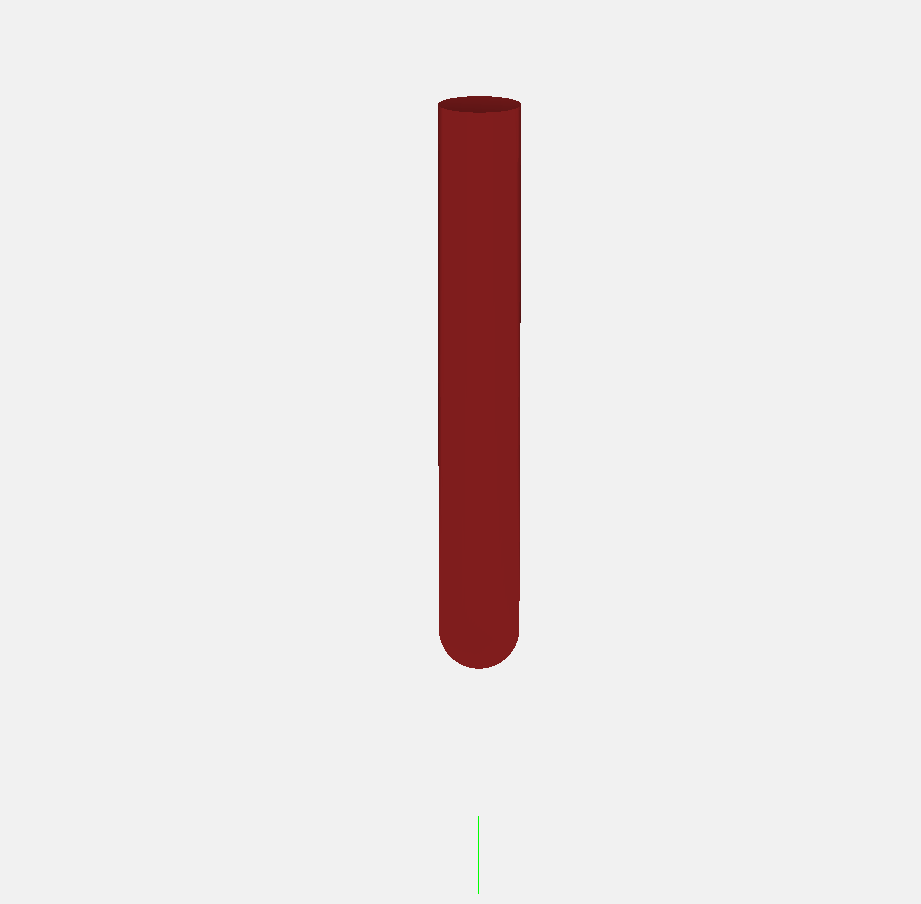
\includegraphics[width=\linewidth/3]{images/tool_ball_202.png}%
           
\includegraphics[width=\linewidth/3]{images/tool_V_301.png}%

\begin{itemize}
\item Square (\#201 and 102) --- able to cut a flat bottom, perpendicular side and right angle
                                 their simple and easily understood geometry makes them a 
                                 standard choice (a radiused form with a flat bottom, often
                                 described as a ``bowl bit'' is not implemented as-of-yet)
\item Ballnose (\#202 and 101) --- rounded, they are the standard choice for concave and 
                                   organic shapes
\item V tooling (\#301, 302 and 390) --- pointed at the tip, they are available in a variety of
                                         angles and diameters and may be used for decorative
                                         V carving, or for chamfering or cutting specific angles
                                         (note that the commonly available radiused form is not
                                         implemented at this time, \emph{e.g.},~\#501 and 502)
\end{itemize}
\end{samepage}

Most tools are easily implemented with concise 3D descriptions which may be connected with a simple \texttt{hull} operation:

The \DescribeRoutine{endmill square} is a simple cylinder:
\lstset{firstnumber=\thegcpy}
\begin{writecode}{a}{gcodepreview.py}{python}
    def endmill_square(self, es_diameter, es_flute_length):
        return cylinder(r1=(es_diameter / 2), r2=(es_diameter / 2), h=es_flute_length, center = False)

\end{writecode}
\addtocounter{gcpy}{3}

The \DescribeRoutine{gcp endmill ball} is modeled as a hemisphere joined with a cylinder:

\lstset{firstnumber=\thegcpy}
\begin{writecode}{a}{gcodepreview.py}{python}
    def gcp_endmill_ball(self, es_diameter, es_flute_length):
        b = sphere(r=(es_diameter / 2))
        s = cylinder(r1=(es_diameter / 2), r2=(es_diameter / 2), h=es_flute_length, center=False)
        p = union(b,s)
        return p.translate([0, 0, (es_diameter / 2)])

\end{writecode}
\addtocounter{gcpy}{6}

The \DescribeRoutine{gcp endmill v} is modeled as a cylinder with a zero width base and a second cylinder for the shaft (note that Python's \verb|math| defaults to radians, hence the need to convert from degrees):

\lstset{firstnumber=\thegcpy}
\begin{writecode}{a}{gcodepreview.py}{python}
    def gcp_endmill_v(self, es_v_angle, es_diameter):
        es_v_angle = math.radians(es_v_angle)
        v = cylinder(r1=0, r2=(es_diameter / 2), h=((es_diameter / 2) / math.tan((es_v_angle / 2))), center=False)
        s = cylinder(r1=(es_diameter / 2), r2=(es_diameter / 2), h=((es_diameter * 8) ), center=False)
        sh = s.translate([0, 0, ((es_diameter / 2) / math.tan((es_v_angle / 2)))])
        return union(v,sh)

\end{writecode}
\addtocounter{gcpy}{7}

\paragraph{Tooling for Keyhole Toolpaths}

\label{para:undercuttooling} Keyhole toolpaths (see: subsection~\ref{subsec:keyholetoolpaths} are intended for use with tooling which projects beyond the the narrower shaft and so will cut usefully underneath the visible surface. Also described as ``undercut'' tooling, but see below.

\begin{samepage}
There are several notable candidates for such tooling:

\noindent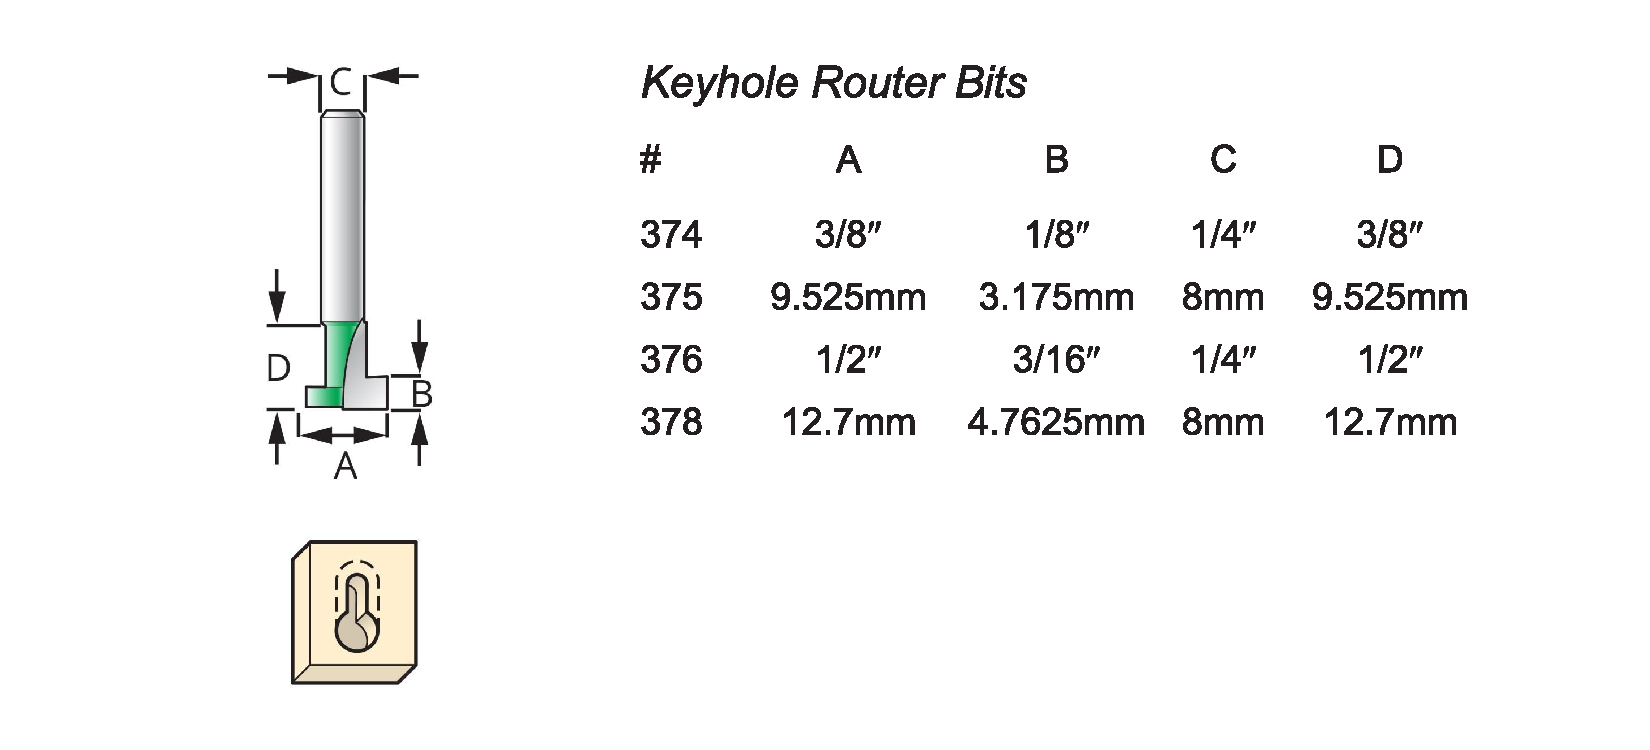
\includegraphics[width=\linewidth]{images/keyhole_router_bits.pdf}%

\begin{itemize}
\item Keyhole tools --- intended to cut slots for retaining hardware used for picture
                        hanging, they may be used to create slots for other purposes
                        Note that it will be necessary to model these twice, once for
                        the shaft, the second time for the actual keyhole cutting
                        \url{https://assetssc.leevalley.com/en-gb/shop/tools/power-tool-accessories/router-bits/30113-keyhole-router-bits}
\item Dovetail cutters --- used for the joinery of the same name, they cut a large
                           area at the bottom which slants up to a narrower region
                           at a defined angle
\item Lollipop cutters --- normally used for 3D work, as their name suggests they are
                           essentially a (cutting) ball on a narrow stick (the tool shaft),
                           they are mentioned here only for compleatness' sake and are not
                           (at this time) implemented
\item Threadmill --- used for cutting threads, normally a single form geometry is used on a CNC.
\end{itemize}
\end{samepage}

\paragraph{Thread mills}

\label{para:threadmills} The implementation of arcs cutting along the Z-axis raises the 
possibility of cutting threads using ``thread mills''. 
See: \url{https://community.carbide3d.com/t/thread-milling-in-metal-on-the-shapeoko-3/5332}

\begin{samepage}
\paragraph{Keyhole}

The \DescribeRoutine{gcp keyhole} is modeled in two parts, first the cutting base:

\lstset{firstnumber=\thegcpy}
\begin{writecode}{a}{gcodepreview.py}{python}
    def gcp_keyhole(self, es_diameter, es_flute_length):
        return cylinder(r1=(es_diameter / 2), r2=(es_diameter / 2), h=es_flute_length, center=False)

\end{writecode}
\addtocounter{gcpy}{3}

\noindent and a second call for an additional cylinder for the shaft will be necessary:

\lstset{firstnumber=\thegcpy}
\begin{writecode}{a}{gcodepreview.py}{python}
    def gcp_keyhole_shaft(self, es_diameter, es_flute_length):
        return cylinder(r1=(es_diameter / 2), r2=(es_diameter / 2), h=es_flute_length, center=False)

\end{writecode}
\addtocounter{gcpy}{3}
\end{samepage}

The \DescribeRoutine{gcp dovetail} is modeled as a cylinder with the differing bottom and top diameters determining the angle (though \verb|dt_angle| is still required as a parameter)

\lstset{firstnumber=\thegcpy}
\begin{writecode}{a}{gcodepreview.py}{python}
    def gcp_dovetail(self, dt_bottomdiameter, dt_topdiameter, dt_height, dt_angle):
        return cylinder(r1=(dt_bottomdiameter / 2), r2=(dt_topdiameter / 2), h= dt_height, center=False)

\end{writecode}
\addtocounter{gcpy}{3}

\paragraph{Concave toolshapes}
\label{para:concavetoolshapes} 
While normal tooling may be represented with a single \texttt{hull} operation betwixt two \textsc{3d} toolshapes (or four in the instance of keyhole tools), concave tooling such as roundover/radius tooling require multiple slices of the tool shape which are then \texttt{hull}ed together. Something of this can be seen in the manual work-around for previewing them: \url{https://community.carbide3d.com/t/using-unsupported-tooling-in-carbide-create-roundover-cove-radius-bits/43723}.

Because it is necessary to divide the tooling into vertical slices and call the hull operation for each slice the tool definitions are tightly coupled with the module. Note that there are two different modules, the public-facing version which includes the tool number:\DescribeRoutine{cutroundover}

\paragraph{Roundover tooling}

\label{para:roundover} It is not possible to represent all tools using tool changes as coded above which require using a \texttt{hull} operation between 3D representations of the tools at the beginning and end points. Tooling which cannot be so represented will be implemented separately below, see paragraph~\ref{para:concavetoolshapes}.

\lstset{firstnumber=\thegcpscad}
\begin{writecode}{a}{gcodepreview.scad}{scad}
module cutroundover(bx, by, bz, ex, ey, ez, radiustn) {
    if (radiustn == 56125) {
        cutroundovertool(bx, by, bz, ex, ey, ez, 0.508/2, 1.531);
    } else if (radiustn == 56142) {
        cutroundovertool(bx, by, bz, ex, ey, ez, 0.508/2, 2.921);
//    } else if (radiustn == 312) {
//        cutroundovertool(bx, by, bz, ex, ey, ez, 1.524/2, 3.175);
    } else if (radiustn == 1570) {
        cutroundovertool(bx, by, bz, ex, ey, ez, 0.507/2, 4.509);
    }
}

\end{writecode}
\addtocounter{gcpscad}{12}

\noindent which then calls the actual \texttt{cutroundovertool} module passing in the tip radius and the radius of the rounding. Note that this module sets its quality relative to the value of \verb|$fn|.

\subsubsection{toolchange}

\noindent and apply the appropriate commands for a \label{subsubsec:toolchange} \DescribeRoutine{toolchange}. Note that it is expected that this code will be updated as needed when new tooling is introduced as additional modules which require specific tooling are added below. 

Note that the comments written out in G-code correspond to that used by the G-code previewing tool CutViewer (which is unfortunately, no longer readily available).

A further concern is that early versions often passed the tool into a module using a parameter. That ceased to be necessary in the 2024.09.03 version of PythonSCAD, and all modules should read the tool \# from \verb|currenttoolnumber()|. Note that this variable has changed names from the original \verb|currenttool| which is now used to store the current tool \emph{shape} (or 3D model).

It is possible that rather than hard-coding the tool definitions, a future update will instead read them in from an external file --- the \texttt{.csv} format used for tool libraries in Carbide Create seems a likely candidate and worth exploring.

Note that there are many varieties of tooling and not all will be implemented, especially in the early versions of this project
 
\paragraph{Selecting Tools}
 
The original implementation created the model for the tool at the current position, wrapping the twain for each end of a given movement in a \verb|hull()| command. This approach will not work within Python, so it will be necessary to instead assign and select the tool as part of the cutting command indirectly by first storing it in the variable \DescribeVariable{currenttoolshape} (if the toolshape will work with the \verb|hull| command) which may be done in this module, or it will be necessary to check for the specific toolnumber in the \verb|cutline| module and handle the tooling in a separate module as is currently done for roundover tooling.

\lstset{firstnumber=\thegcpy}
\begin{writecode}{a}{gcodepreview.py}{python}
    def currenttool(self):
#        global currenttoolshape
        return self.currenttoolshape

\end{writecode}
\addtocounter{gcpy}{4}

Note that it will also be necessary to write out a tool description compatible with the program CutViewer as a G-code comment so that it may be used as a 3D previewer for the G-code for tool changes in G-code. Several forms are available:

\paragraph{Square and ball nose (including tapered ball nose)}

\begin{verbatim}
TOOL/MILL, Diameter, Corner radius, Height, Taper Angle
\end{verbatim}

\paragraph{Roundover (corner rounding)}

\begin{verbatim}
TOOL/CRMILL, Diameter1, Diameter2,Radius, Height, Length
\end{verbatim}

Unfortunately, tools which support undercuts such as dovetails are not supported (CAMotics will work for such tooling).

\lstset{firstnumber=\thegcpy}
\begin{writecode}{a}{gcodepreview.py}{python}
    def toolchange(self,tool_number,speed):
#        global currenttoolshape
        self.currenttoolshape = self.endmill_square(0.001, 0.001)    
            
        self.settool(tool_number)
        if (self.generategcode == True):
            self.writegc("(Toolpath)")
            self.writegc("M05")
        if (tool_number == 201):
            self.writegc("(TOOL/MILL,6.35, 0.00, 0.00, 0.00)")
            self.currenttoolshape = self.endmill_square(6.35, 19.05)
        elif (tool_number == 102):
            self.writegc("(TOOL/MILL,3.175, 0.00, 0.00, 0.00)")
            self.currenttoolshape = self.endmill_square(3.175, 12.7)
        elif (tool_number == 112):
            self.writegc("(TOOL/MILL,1.5875, 0.00, 0.00, 0.00)")
            self.currenttoolshape = self.endmill_square(1.5875, 6.35)
        elif (tool_number == 122):
            self.writegc("(TOOL/MILL,0.79375, 0.00, 0.00, 0.00)")
            self.currenttoolshape = self.endmill_square(0.79375, 1.5875)
        elif (tool_number == 202):
            self.writegc("(TOOL/MILL,6.35, 3.175, 0.00, 0.00)")
            self.currenttoolshape = self.gcp_endmill_ball(6.35, 19.05)
        elif (tool_number == 101):
            self.writegc("(TOOL/MILL,3.175, 1.5875, 0.00, 0.00)")
            self.currenttoolshape = self.gcp_endmill_ball(3.175, 12.7)
        elif (tool_number == 111):
            self.writegc("(TOOL/MILL,1.5875, 0.79375, 0.00, 0.00)")
            self.currenttoolshape = self.gcp_endmill_ball(1.5875, 6.35)
        elif (tool_number == 121):
            self.writegc("(TOOL/MILL,3.175, 0.79375, 0.00, 0.00)")
            self.currenttoolshape = self.gcp_endmill_ball(0.79375, 1.5875)
        elif (tool_number == 327):
            self.writegc("(TOOL/MILL,0.03, 0.00, 13.4874, 30.00)")
            self.currenttoolshape = self.gcp_endmill_v(60, 26.9748)
        elif (tool_number == 301):
            self.writegc("(TOOL/MILL,0.03, 0.00, 6.35, 45.00)")
            self.currenttoolshape = self.gcp_endmill_v(90, 12.7)
        elif (tool_number == 302):
            self.writegc("(TOOL/MILL,0.03, 0.00, 10.998, 30.00)")
            self.currenttoolshape = self.gcp_endmill_v(60, 12.7)
        elif (tool_number == 390):
            self.writegc("(TOOL/MILL,0.03, 0.00, 1.5875, 45.00)")
            self.currenttoolshape = self.gcp_endmill_v(90, 3.175)
        elif (tool_number == 374):
            self.writegc("(TOOL/MILL,9.53, 0.00, 3.17, 0.00)")
        elif (tool_number == 375):
            self.writegc("(TOOL/MILL,9.53, 0.00, 3.17, 0.00)")
        elif (tool_number == 376):
            self.writegc("(TOOL/MILL,12.7, 0.00, 4.77, 0.00)")
        elif (tool_number == 378):
            self.writegc("(TOOL/MILL,12.7, 0.00, 4.77, 0.00)")
        elif (tool_number == 814):
            self.writegc("(TOOL/MILL,12.7, 6.367, 12.7, 0.00)")
            #dt_bottomdiameter, dt_topdiameter, dt_height, dt_angle)
            #https://www.leevalley.com/en-us/shop/tools/power-tool-accessories/router-bits/30172-dovetail-bits?item=18J1607
            self.currenttoolshape = self.gcp_dovetail(12.7, 6.367, 12.7, 14)
        elif (tool_number == 56125):#0.508/2, 1.531
            self.writegc("(TOOL/CRMILL, 0.508, 6.35, 3.175, 7.9375, 3.175)")
        elif (tool_number == 56142):#0.508/2, 2.921
            self.writegc("(TOOL/CRMILL, 0.508, 3.571875, 1.5875, 5.55625, 1.5875)")
#        elif (tool_number == 312):#1.524/2, 3.175
#            self.writegc("(TOOL/CRMILL, Diameter1, Diameter2,Radius, Height, Length)")
        elif (tool_number == 1570):#0.507/2, 4.509
            self.writegc("(TOOL/CRMILL, 0.17018, 9.525, 4.7625, 12.7, 4.7625)")
\end{writecode}
\addtocounter{gcpy}{65}
 
\noindent With the tools delineated, the module is closed out and the toolchange information written into the G-code as well as the command to start the spindle at the specified speed.
 
\lstset{firstnumber=\thegcpy}
\begin{writecode}{a}{gcodepreview.py}{python}
        self.writegc("M6T",str(tool_number))
        self.writegc("M03S",str(speed))

\end{writecode}
\addtocounter{gcpy}{3}

For example:

\begin{verbatim}
toolchange(small_square_tool_num,speed);
\end{verbatim}

\noindent (the assumption is that all speed rates in a file will be the same, so as to account for the most frequent use case of a trim router with speed controlled by a dial setting)

\subsubsection{tooldiameter}

It will also be necessary to be able to provide the diameter of the current tool. Arguably, this would be much easier using an object-oriented programming style/dot notation.

One aspect of tool parameters which will need to be supported is shapes which create different profiles based on how deeply the tool is cutting into the surface of the material at a given point. To accommodate this, it will be necessary to either track the thickness of uncut material at any given point, or, to specify the depth of cut as a parameter which is what the initial version will implement.

The public-facing OpenSCAD code, \DescribeRoutine{tool diameter} simply calls the matching OpenSCAD module which wraps the Python code:
 
\lstset{firstnumber=\thegcpscad}
\begin{writecode}{a}{gcodepreview.scad}{scad}
function tool_diameter(td_tool, td_depth) = otool_diameter(td_tool, td_depth);

\end{writecode}
\addtocounter{gcpscad}{2}

\noindent the matching OpenSCAD function, \DescribeSubroutine{tool diameter}{otool diameter} calls the Python function:

\lstset{firstnumber=\thepyscad}
\begin{writecode}{a}{pygcodepreview.scad}{scad}
function otool_diameter(td_tool, td_depth) = ptool_diameter(td_tool, td_depth);

\end{writecode}
\addtocounter{pyscad}{2}
 
\noindent the Python code, \DescribeSubroutine{tool diameter}{ptool diameter} returns 
appropriate values based on the specified tool number and depth:
 
\lstset{firstnumber=\thegcpy}
\begin{writecode}{a}{gcodepreview.py}{python}
    def tool_diameter(self, ptd_tool, ptd_depth):
# Square 122,112,102,201
        if ptd_tool == 122:
            return 0.79375
        if ptd_tool == 112:
            return 1.5875
        if ptd_tool == 102:
            return 3.175
        if ptd_tool == 201:
            return 6.35
# Ball 121,111,101,202
        if ptd_tool == 122:
            if ptd_depth > 0.396875:
                return 0.79375
            else:
                return ptd_tool
        if ptd_tool == 112:
            if ptd_depth > 0.79375:
                return 1.5875
            else:
                return ptd_tool
        if ptd_tool == 101:
            if ptd_depth > 1.5875:
                return 3.175
            else:
                return ptd_tool
        if ptd_tool == 202:
            if ptd_depth > 3.175:
                return 6.35
            else:
                return ptd_tool
# V 301, 302, 390
        if ptd_tool == 301:
            return ptd_tool
        if ptd_tool == 302:
            return ptd_tool
        if ptd_tool == 390:
            return ptd_tool
# Keyhole
        if ptd_tool == 374:
            if ptd_depth < 3.175:
                return 9.525
            else:
                return 6.35
        if ptd_tool == 375:
            if ptd_depth < 3.175:
                return 9.525
            else:
                return 8
        if ptd_tool == 376:
            if ptd_depth < 4.7625:
                return 12.7
            else:
                return 6.35
        if ptd_tool == 378:
            if ptd_depth < 4.7625:
                return 12.7
            else:
                return 8
# Dovetail
        if ptd_tool == 814:
            if ptd_depth > 12.7:
                return 6.35
            else:
                return 12.7

\end{writecode}
\addtocounter{gcpy}{66}

Since it is often necessary to utilise the radius of the tool, an additional command, \DescribeRoutine{tool radius} to return this value is worthwhile:
 
\lstset{firstnumber=\thegcpy}
\begin{writecode}{a}{gcodepreview.py}{python}
    def tool_radius(self, ptd_tool, ptd_depth):
        tr = self.tool_diameter(ptd_tool, ptd_depth)/2
        return tr

\end{writecode}
\addtocounter{gcpy}{4}
 
(Note that where values are not fully calculated values currently the passed in tool number is returned which will need to be replaced with code which calculates the appropriate values.)

\subsubsection{Feeds and Speeds}

There are several possibilities for handling feeds and speeds. Currently, base values for \DescribeVariable{feed}, \DescribeVariable{plunge}, and \DescribeVariable{speed} are used, which may then be adjusted using various \verb|<tooldescriptor>_ratio| values, as an acknowledgement of the likelihood of a trim router being used as a spindle, the assumption is that the \texttt{speed} will remain unchanged.

One notable possibility for the future would be to load it from the .csv files used for User tool libraries in Carbide Create. Ideally, any use of such values in modules would be such that some other scheme could replace that usage with minimal editing and updating.

The tools which need to be calculated thus are those in addition to the \verb|large_square| tool:

\begin{itemize}
\item \verb|small_square_ratio|
\item \verb|small_ball_ratio|
\item \verb|large_ball_ratio|
\item \verb|small_V_ratio|
\item \verb|large_V_ratio|
\item \verb|KH_ratio|
\item \verb|DT_ratio|
\end{itemize}

\begin{samepage}
\subsection{OpenSCAD File Handling}
 
For writing to files it will be necessary to have commands: 
\DescribeSubroutine{opengcodefile}{popengcodefile}, 
\DescribeSubroutine{opendxffile}{popendxffile}, 
\DescribeRoutine{popendxflgsqfile}, 
\DescribeRoutine{popendxfsmsqfile}, 
\DescribeRoutine{popendxflgblfile}, 
\DescribeRoutine{popendxfsmblfile},  
\DescribeRoutine{popendxflgVfile}, and 
\DescribeRoutine{popendxfsmVfile}.
%\DescribeRoutine{popensvgfile}
There is a separate function for each type of file, and for DXFs, there are multiple file instances, one for each combination of different type and size of tool which it is expected a project will work with. Each such file will be suffixed with the tool number.

Integrating G-code and \textsc{dxf} generation with everything else would be ideal, but will require ensuring that each command which moves the tool creates a matching command for both files.

\lstset{firstnumber=\thegcpy}
\begin{writecode}{a}{gcodepreview.py}{python}
#def popengcodefile(fn):
#    global f
#    f = open(fn, "w")
#
#def popendxffile(fn):
#    global dxf
#    dxf = open(fn, "w")
#
#def popendxflgblfile(fn):
#    global dxflgbl
#    dxflgbl = open(fn, "w")
#
#def popendxflgsqfile(fn):
#    global dxflgsq
#    dxflgsq = open(fn, "w")
#
#def popendxflgVfile(fn):
#    global dxflgV
#    dxflgV = open(fn, "w")
#
#def popendxfsmblfile(fn):
#    global dxfsmbl
#    dxfsmbl = open(fn, "w")
#
#def popendxfsmsqfile(fn):
#    global dxfsmsq
#    dxfsmsq = open(fn, "w")
#
#def popendxfsmVfile(fn):
#    global dxfsmV
#    dxfsmV = open(fn, "w")
#
#def popendxfKHfile(fn):
#    global dxfKH
#    dxfKH = open(fn, "w")
#
#def popendxfDTfile(fn):
#    global dxfDT
#    dxfDT = open(fn, "w")
#
\end{writecode}
\addtocounter{gcpy}{40}
%def popensvgfile(fn):
%    global svg
%    svg = open(fn, "w")
\end{samepage}

%\DescribeRoutine{oopensvgfile}
There will need to be matching OpenSCAD modules 
\DescribeSubroutine{opengcodefile}{oopengcodefile}, and
\DescribeSubroutine{opendxffile}{oopendxffile}, 
for the Python functions.

\lstset{firstnumber=\thepyscad}
\begin{writecode}{a}{pygcodepreview.scad}{scad}
module oopengcodefile(fn) {
    popengcodefile(fn);
}

module oopendxffile(fn) {
//    echo(fn);
    popendxffile(fn);
}

module oopendxflgblfile(fn) {
    popendxflgblfile(fn);
}

module oopendxflgsqfile(fn) {
    popendxflgsqfile(fn);
}

module oopendxflgVfile(fn) {
    popendxflgVfile(fn);
}

module oopendxfsmblfile(fn) {
    popendxfsmblfile(fn);
}

module oopendxfsmsqfile(fn) {
//    echo(fn);
    popendxfsmsqfile(fn);
}

module oopendxfsmVfile(fn) {
    popendxfsmVfile(fn);
}

module oopendxfKHfile(fn) {
    popendxfKHfile(fn);
}

module oopendxfDTfile(fn) {
    popendxfDTfile(fn);
}

\end{writecode}
\addtocounter{pyscad}{42}
%module oopensvgfile(fn) {
%    popensvgfile(fn);
%}

With matching OpenSCAD commands: \DescribeRoutine{opengcodefile}%\DescribeRoutine{opensvgfile}
 
\lstset{firstnumber=\thegcpscad}
\begin{writecode}{a}{gcodepreview.scad}{scad}
module opengcodefile(fn) {
if (generategcode == true) {
    oopengcodefile(fn);
//    echo(fn);
    owritecomment(fn);
    }
}

\end{writecode}
\addtocounter{gcpscad}{8}
%module opensvgfile(fn) {
%if (generatesvg == true) {
%    oopensvgfile(fn);
%    echo(fn);
%    svgwriteone(str("<?xml version=",chr(34),"1.0",chr(34)," encoding=",chr(34),"UTF-8",chr(34)," standalone=",chr(34),"no",chr(34),"?> "));
%//    writesvglineend();
%svgwriteone(str("<svg  version=",chr(34),"1.1",chr(34)," xmlns=",chr(34),"http://www.w3.org/2000/svg",chr(34)," width=",chr(34),stockXwidth*3.77953,"px",chr(34)," height=",chr(34),stockYheight*3.77953,"px",chr(34),"> "));
%//<path d="M755.906 0 L755.906 377.953 L0 377.953 L0 0 L755.906 0 Z " stroke="black" stroke-width="1" fill="none" /> 
%svgwriteone(str("<path d=",chr(34),"M",stockXwidth*3.77953," 0 L",stockXwidth*3.77953," ",stockYheight*3.77953," L0 ",stockYheight*3.77953," L0 0 L",stockXwidth*3.77953," 0 Z ",chr(34)," stroke=",chr(34),"black",chr(34)," stroke-width=",chr(34),"1",chr(34)," fill=",chr(34),"none",chr(34)," /> "));
%}
%}

\subsubsection{Writing to files}
 
When the command to open \verb|.dxf| files is called it is passed all of the variables for the various tool types/sizes, and based on a value being greater than zero, the matching file is opened, and in addition, the main \textsc{dxf} which is always written to is opened as well. On the gripping hand, each element which may be written to a \textsc{dxf} file will have a user module as well as an internal module which will be called by it so as to write to the file for the current tool. It will be necessary for the \DescribeRoutine{dxfwrite} command to evaluate the tool number which is passed in, and to use an appropriate command or set of commands to then write out to the appropriate file for a given tool (if positive) or not do anything (if zero), and to write to the master file if a negative value is passed in (this allows the various DXF template commands to be written only once and then called at need).

\noindent has a matching command each tool/size combination:

\begin{itemize}
\item Ball nose, large (lgbl) \DescribeRoutine{writedxflgbl}
\item Ball nose, small (smbl) \DescribeRoutine{writedxfsmbl}
\item Square, large (lgsq) \DescribeRoutine{writedxflgsq}
\item Square, small (smsq) \DescribeRoutine{writedxfsmsq}
\item V, large (lgV) \DescribeRoutine{writedxflgV}
\item V, small (smV) \DescribeRoutine{writedxfsmV}
\item Keyhole (KH) \DescribeRoutine{writedxfKH}
\item Dovetail (DT) \DescribeRoutine{writedxfDT}
\end{itemize}
 
\lstset{firstnumber=\thegcpy}
\begin{writecode}{a}{gcodepreview.py}{python}
#def writedxflgbl(*arguments):
#    line_to_write = ""
#    for element in arguments:
#        line_to_write += element
#    dxflgbl.write(line_to_write)
#    print(line_to_write)
#    dxflgbl.write("\n")
#
#def writedxflgsq(*arguments):
#    line_to_write = ""
#    for element in arguments:
#        line_to_write += element
#    dxflgsq.write(line_to_write)
#    print(line_to_write)
#    dxflgsq.write("\n")
#
#def writedxflgV(*arguments):
#    line_to_write = ""
#    for element in arguments:
#        line_to_write += element
#    dxflgV.write(line_to_write)
#    print(line_to_write)
#    dxflgV.write("\n")
#
#def writedxfsmbl(*arguments):
#    line_to_write = ""
#    for element in arguments:
#        line_to_write += element
#    dxfsmbl.write(line_to_write)
#    print(line_to_write)
#    dxfsmbl.write("\n")
#
#def writedxfsmsq(*arguments):
#    line_to_write = ""
#    for element in arguments:
#        line_to_write += element
#    dxfsmsq.write(line_to_write)
#    print(line_to_write)
#    dxfsmsq.write("\n")
#
#def writedxfsmV(*arguments):
#    line_to_write = ""
#    for element in arguments:
#        line_to_write += element
#    dxfsmV.write(line_to_write)
#    print(line_to_write)
#    dxfsmV.write("\n")
#
#def writedxfKH(*arguments):
#    line_to_write = ""
#    for element in arguments:
#        line_to_write += element
#    dxfKH.write(line_to_write)
#    print(line_to_write)
#    dxfKH.write("\n")
#
#def writedxfDT(*arguments):
#    line_to_write = ""
#    for element in arguments:
#        line_to_write += element
#    dxfDT.write(line_to_write)
#    print(line_to_write)
#    dxfDT.write("\n")
#
\end{writecode}
\addtocounter{gcpy}{64}
%def writesvg(*arguments):
%    line_to_write = ""
%    for element in arguments:
%        line_to_write += element
%    svg.write(line_to_write)
%    print(line_to_write)
%
%def pwritesvgline():
%    svg.write("\n")
 
Separate OpenSCAD modules, 
\DescribeRoutine{owritecomment}, 
\DescribeRoutine{dxfwriteone}, 
\DescribeRoutine{dxfwritelgbl}, 
\DescribeRoutine{dxfwritelgsq}, 
\DescribeRoutine{dxfwritelgV}, 
\DescribeRoutine{dxfwritesmbl}, 
\DescribeRoutine{dxfwritesmsq}, and
\DescribeRoutine{dxfwritesmV} 
will be used for either writing out comments in G-code (.nc) files or adding to a DXF file --- for each different tool in a file there will be a matching module to write to it.
 
\lstset{firstnumber=\thepyscad}
\begin{writecode}{a}{pygcodepreview.scad}{scad}
module owritecomment(comment) {
    writeln("(",comment,")");
}

module dxfwriteone(first) {
    writedxf(first);
//    writeln(first);
//    echo(first);
}

module dxfwritelgbl(first) {
    writedxflgbl(first);
}

module dxfwritelgsq(first) {
    writedxflgsq(first);
}

module dxfwritelgV(first) {
    writedxflgV(first);
}

module dxfwritesmbl(first) {
    writedxfsmbl(first);
}

module dxfwritesmsq(first) {
    writedxfsmsq(first);
}

module dxfwritesmV(first) {
    writedxfsmV(first);
}

module dxfwriteKH(first) {
    writedxfKH(first);
}

module dxfwriteDT(first) {
    writedxfDT(first);
}

\end{writecode}
\addtocounter{pyscad}{42}
%module svgwriteone(first) {
%    writesvg(first);
%}
%
%module writesvglineend(first) {
%    pwritesvgline();
%}

Since it is not convenient to stitch together and then write out multiple elements, the most expedient thing to do is to have discrete commands for each possible number of arguments, one through thirteen, \DescribeRoutine{owrite...}
 
\lstset{firstnumber=\thepyscad}
\begin{writecode}{a}{pygcodepreview.scad}{scad}
module owriteone(first) {
    writeln(first);
}

module owritetwo(first, second) {
    writeln(first, second);
}

module owritethree(first, second, third) {
    writeln(first, second, third);
}

module owritefour(first, second, third, fourth) {
    writeln(first, second, third, fourth);
}

module owritefive(first, second, third, fourth, fifth) {
    writeln(first, second, third, fourth, fifth);
}

module owritesix(first, second, third, fourth, fifth, sixth) {
    writeln(first, second, third, fourth, fifth, sixth);
}

module owriteseven(first, second, third, fourth, fifth, sixth, seventh) {
    writeln(first, second, third, fourth, fifth, sixth, seventh);
}

module owriteeight(first, second, third, fourth, fifth, sixth, seventh,eighth) {
    writeln(first, second, third, fourth, fifth, sixth, seventh,eighth);
}

module owritenine(first, second, third, fourth, fifth, sixth, seventh, eighth, ninth) {
    writeln(first, second, third, fourth, fifth, sixth, seventh, eighth, ninth);
}

module owriteten(first, second, third, fourth, fifth, sixth, seventh, eighth, ninth, tenth) {
    writeln(first, second, third, fourth, fifth, sixth, seventh, eighth, ninth, tenth);
}

module owriteeleven(first, second, third, fourth, fifth, sixth, seventh, eighth, ninth, tenth, eleventh) {
    writeln(first, second, third, fourth, fifth, sixth, seventh, eighth, ninth, tenth, eleventh);
}

module owritetwelve(first, second, third, fourth, fifth, sixth, seventh, eighth, ninth, tenth, eleventh, twelfth) {
    writeln(first, second, third, fourth, fifth, sixth, seventh, eighth, ninth, tenth, eleventh, twelfth);
}

module owritethirteen(first, second, third, fourth, fifth, sixth, seventh, eighth, ninth, tenth, eleventh, twelfth, thirteenth) {
    writeln(first, second, third, fourth, fifth, sixth, seventh, eighth, ninth, tenth, eleventh, twelfth, thirteenth);
}

\end{writecode}
\addtocounter{pyscad}{52}
 
\paragraph{Writing to DXFs}%\DescribeRoutine{writesvgline}

This module requires that the tool number be passed in, and after writing out \DescribeRoutine{dxfpreamble}, that value will be used to write out to the appropriate file with a series of \texttt{if} statements.
 
\lstset{firstnumber=\thegcpy}
\begin{writecode}{a}{gcodepreview.py}{python}
    def dxfpreamble(self, tn):
#        self.writedxf(tn,str(tn))
        self.writedxf(tn,"0")
        self.writedxf(tn,"SECTION")
        self.writedxf(tn,"2")
        self.writedxf(tn,"ENTITIES")

\end{writecode}
\addtocounter{gcpy}{7}
 
\paragraph{DXF Lines and Arcs}%
 
There are two notable elements which may be written to a DXF:

\begin{itemize}
 \item a line: LWPOLYLINE is one possible implementation: \DescribeRoutine{dxfbpl} 
       %\DescribeRoutine{beginpolyline},
 \item ARC --- a notable option would be for the arc to close on itself, creating a circle:
       \DescribeRoutine{dxfarc}
\end{itemize}
 
DXF orders arcs counter-clockwise:

\noindent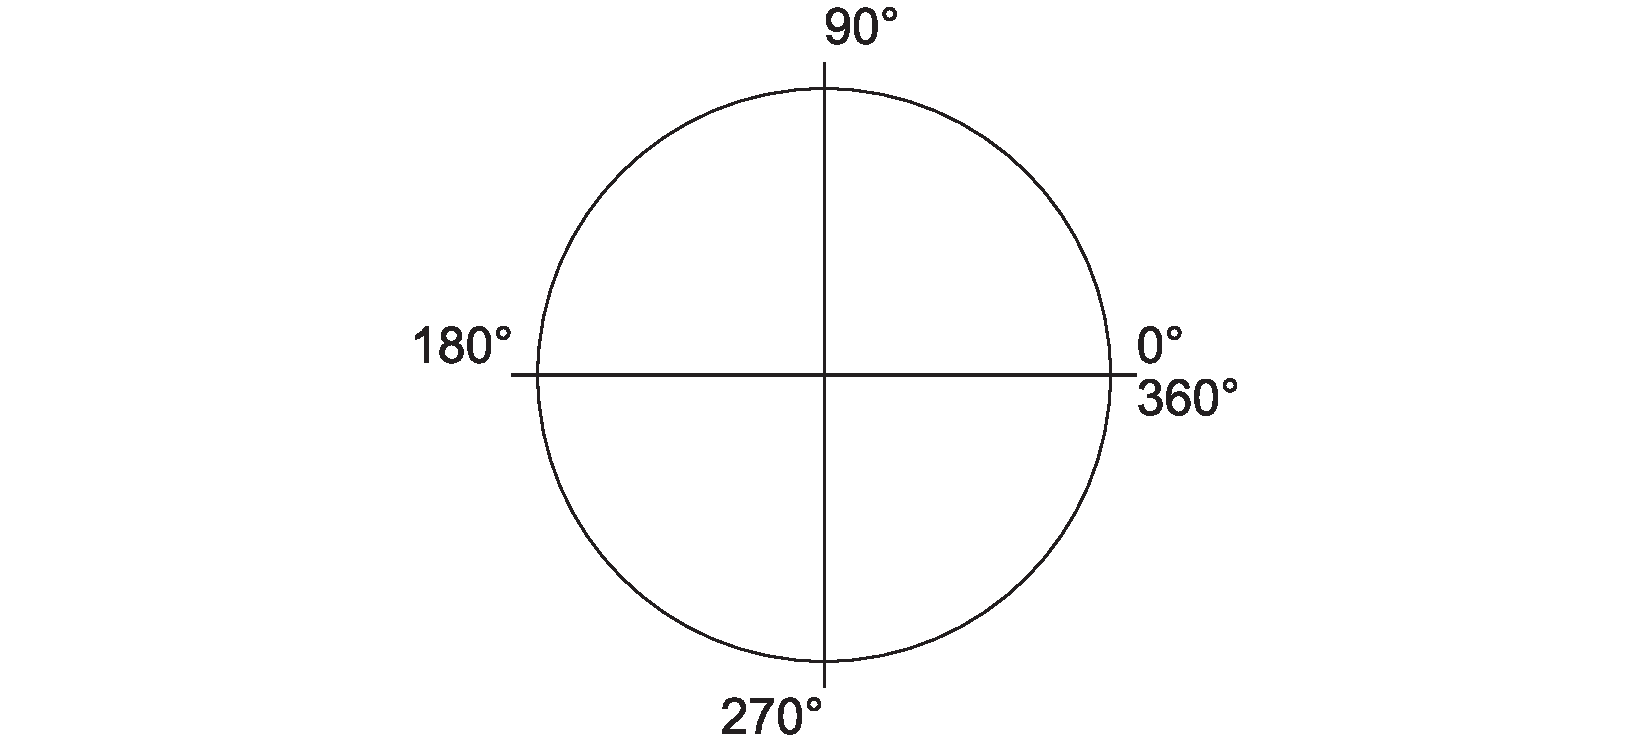
\includegraphics[width=\linewidth]{images/arcs_circle_degrees.pdf}%

Note that arcs of greater than 90 degrees are not rendered accurately, so, for the sake of precision, they should be limited to a swing of 90 degrees or less. Further note that 4 arcs may be stitched together to make a circle:
 
\begin{verbatim}
           dxfarc(10, 10, 5,   0,  90, small_square_tool_num);
           dxfarc(10, 10, 5,  90, 180, small_square_tool_num);
           dxfarc(10, 10, 5, 180, 270, small_square_tool_num);
           dxfarc(10, 10, 5, 270, 360, small_square_tool_num);
\end{verbatim}
 
A further refinement would be to connect multiple line segments/arcs into a larger polyline, but since most CAM tools implicitly join elements on import, that is not necessary.
 
There are three possible interactions for DXF elements and toolpaths:

\begin{itemize}
 \item describe the motion of the tool
 \item define a perimeter of an area which will be cut by a tool
 \item define a centerpoint for a specialty toolpath such as Drill or Keyhhole
\end{itemize}
 
\noindent and it is possible that multiple such elements could be instantiated for a given toolpath.
 
When writing out to a \textsc{dxf} file there is a pair of commands, a public facing command which takes in a tool number in addition to the coordinates which then writes out to the main \textsc{dxf} file and then calls an internal command to which repeats the call with the tool number so as to write it out to the matching file.

\lstset{firstnumber=\thegcpy}
\begin{writecode}{a}{gcodepreview.py}{python}
    def dxfline(self, tn, xbegin,ybegin,xend,yend):
        self.writedxf(tn,"0")
        self.writedxf(tn,"LWPOLYLINE")
        self.writedxf(tn,"90")
        self.writedxf(tn,"2")
        self.writedxf(tn,"70")
        self.writedxf(tn,"0")
        self.writedxf(tn,"43")
        self.writedxf(tn,"0")
        self.writedxf(tn,"10")
        self.writedxf(tn,str(xbegin))
        self.writedxf(tn,"20")
        self.writedxf(tn,str(ybegin))
        self.writedxf(tn,"10")
        self.writedxf(tn,str(xend))
        self.writedxf(tn,"20")
        self.writedxf(tn,str(yend))

\end{writecode}
\addtocounter{gcpy}{18}

The original implementation of polylines worked, but may be removed.
 
\lstset{firstnumber=\thegcpscad}
\begin{writecode}{a}{gcodepreview.scad}{scad}
module dxfbpl(tn,bx,by) {
    dxfwrite(tn,"0");
    dxfwrite(tn,"POLYLINE");
    dxfwrite(tn,"8");
    dxfwrite(tn,"default");
    dxfwrite(tn,"66");
    dxfwrite(tn,"1");
    dxfwrite(tn,"70");
    dxfwrite(tn,"0");
    dxfwrite(tn,"0");
    dxfwrite(tn,"VERTEX");
    dxfwrite(tn,"8");
    dxfwrite(tn,"default");
    dxfwrite(tn,"70");
    dxfwrite(tn,"32");
    dxfwrite(tn,"10");
    dxfwrite(tn,str(bx));
    dxfwrite(tn,"20");
    dxfwrite(tn,str(by));
}

module beginpolyline(bx,by,bz) {
if (generatedxf == true) {
    dxfwriteone("0");
    dxfwriteone("POLYLINE");
    dxfwriteone("8");
    dxfwriteone("default");
    dxfwriteone("66");
    dxfwriteone("1");
    dxfwriteone("70");
    dxfwriteone("0");
    dxfwriteone("0");
    dxfwriteone("VERTEX");
    dxfwriteone("8");
    dxfwriteone("default");
    dxfwriteone("70");
    dxfwriteone("32");
    dxfwriteone("10");
    dxfwriteone(str(bx));
    dxfwriteone("20");
    dxfwriteone(str(by));
    dxfbpl(current_tool(),bx,by);}
}

module dxfapl(tn,bx,by) {
    dxfwrite(tn,"0");
    dxfwrite(tn,"VERTEX");
    dxfwrite(tn,"8");
    dxfwrite(tn,"default");
    dxfwrite(tn,"70");
    dxfwrite(tn,"32");
    dxfwrite(tn,"10");
    dxfwrite(tn,str(bx));
    dxfwrite(tn,"20");
    dxfwrite(tn,str(by));
}

module addpolyline(bx,by,bz) {
if (generatedxf == true) {
    dxfwriteone("0");
    dxfwriteone("VERTEX");
    dxfwriteone("8");
    dxfwriteone("default");
    dxfwriteone("70");
    dxfwriteone("32");
    dxfwriteone("10");
    dxfwriteone(str(bx));
    dxfwriteone("20");
    dxfwriteone(str(by));
    dxfapl(current_tool(),bx,by);
    }
}

module dxfcpl(tn) {
    dxfwrite(tn,"0");
    dxfwrite(tn,"SEQEND");
}

module closepolyline() {
  if (generatedxf == true) {
    dxfwriteone("0");
    dxfwriteone("SEQEND");
    dxfcpl(current_tool());
  }
}

module writecomment(comment) {
  if (generategcode == true) {
    owritecomment(comment);
  }
}

\end{writecode}
\addtocounter{gcpscad}{92}
 
At the end of the project it will be necessary to close each file using the commands: 
\DescribeSubroutine{closegcodefile}{pclosegcodefile}, and
\DescribeRoutine{closedxffile}. %\DescribeRoutine{pclosesvgfile}
In some instances it may be necessary to write additional information, depending on the file format. Note that these commands will need to be within the \verb|gcodepreview class|.
 
\lstset{firstnumber=\thegcpy}
\begin{writecode}{a}{gcodepreview.py}{python}
    def dxfpostamble(self,tn):
#        self.writedxf(tn,str(tn))
        self.writedxf(tn,"0")
        self.writedxf(tn,"ENDSEC")
        self.writedxf(tn,"0")
        self.writedxf(tn,"EOF")
        
\end{writecode}
\addtocounter{gcpy}{7}

\lstset{firstnumber=\thegcpy}
\begin{writecode}{a}{gcodepreview.py}{python}
    def gcodepostamble(self):
        self.writegc("Z12.700")
        self.writegc("M05")
        self.writegc("M02")
        
\end{writecode}
\addtocounter{gcpy}{5}


It will be necessary to call the dxfpostamble (with appropriate checks and trappings so as to ensure that each dxf file is ended and closed so as to be valid.
 
\lstset{firstnumber=\thegcpy}
\begin{writecode}{a}{gcodepreview.py}{python}
    def closegcodefile(self):
        self.gcodepostamble()
        self.gc.close()

    def closedxffile(self):
        if self.generatedxf == True:
#            global dxfclosed
            self.dxfclosed = True
            self.dxfpostamble(-1)
            self.dxf.close()
    
    def closedxffiles(self):
        if self.generatedxfs == True:
            if (self.large_square_tool_num > 0):
                self.dxfpostamble(self.large_square_tool_num)
            if (self.small_square_tool_num > 0):
                self.dxfpostamble(self.small_square_tool_num)
            if (self.large_ball_tool_num > 0):
                self.dxfpostamble(self.large_ball_tool_num)
            if (self.small_ball_tool_num > 0):
                self.dxfpostamble(self.small_ball_tool_num)
            if (self.large_V_tool_num > 0):
                self.dxfpostamble(self.large_V_tool_num)
            if (self.small_V_tool_num > 0):
                self.dxfpostamble(self.small_V_tool_num)
            if (self.DT_tool_num > 0):
                self.dxfpostamble(self.DT_tool_num)
            if (self.KH_tool_num > 0):
                self.dxfpostamble(self.KH_tool_num)
            if (self.Roundover_tool_num > 0):
                self.dxfpostamble(self.Roundover_tool_num)
            if (self.MISC_tool_num > 0):
                self.dxfpostamble(self.MISC_tool_num)
                
            if (self.large_square_tool_num > 0):
                self.dxflgsq.close()
            if (self.small_square_tool_num > 0):
                self.dxfsmsq.close()
            if (self.large_ball_tool_num > 0):
                self.dxflgbl.close()
            if (self.small_ball_tool_num > 0):
                self.dxfsmbl.close()
            if (self.large_V_tool_num > 0):
                self.dxflgV.close()
            if (self.small_V_tool_num > 0):
                self.dxfsmV.close()
            if (self.DT_tool_num > 0):
                self.dxfDT.close()
            if (self.KH_tool_num > 0):
                self.dxfKH.close()
            if (self.Roundover_tool_num > 0):
                self.dxfRt.close()
            if (self.MISC_tool_num > 0):
                self.dxfMt.close()

\end{writecode}
\addtocounter{gcpy}{55}
%def pclosesvgfile():
%    svg.close()
%

In addition to the Python forms, there will need to be matching OpenSCAD commands to call them:
\DescribeSubroutine{closegcodefile}{oclosegcodefile}, and 
\DescribeSubroutine{closedxffile}{oclosedxffile}.
%\DescribeSubroutine{oclosedxflgblfile}

\lstset{firstnumber=\thepyscad}
\begin{writecode}{a}{pygcodepreview.scad}{scad}
module oclosegcodefile() {
    pclosegcodefile();
}

module oclosedxffile() {
    pclosedxffile();
}

module oclosedxflgblfile() {
    pclosedxflgblfile();
}

module oclosedxflgsqfile() {
    pclosedxflgsqfile();
}

module oclosedxflgVfile() {
    pclosedxflgVfile();
}

module oclosedxfsmblfile() {
    pclosedxfsmblfile();
}

module oclosedxfsmsqfile() {
    pclosedxfsmsqfile();
}

module oclosedxfsmVfile() {
    pclosedxfsmVfile();
}

module oclosedxfDTfile() {
    pclosedxfDTfile();
}

module oclosedxfKHfile() {
    pclosedxfKHfile();
}

\end{writecode}
\addtocounter{pyscad}{40}
%module oclosesvgfile() {
%    pclosesvgfile();
%}
%

The commands: \DescribeRoutine{closegcodefile}, and \DescribeRoutine{closedxffile} are used to close the files at the end of a program. For efficiency, each references the command: \DescribeRoutine{dxfpostamble} which when called provides the boilerplate needed at the end of their respective files.

\lstset{firstnumber=\thegcpscad}
\begin{writecode}{a}{gcodepreview.scad}{scad}
module closegcodefile() {
  if (generategcode == true) {
    owriteone("M05");
    owriteone("M02");
    oclosegcodefile();
  }
}

module dxfpostamble(arg) {
    dxfwrite(arg,"0");
    dxfwrite(arg,"ENDSEC");
    dxfwrite(arg,"0");
    dxfwrite(arg,"EOF");
}

module closedxffile() {
  if (generatedxf == true) {
    dxfwriteone("0");
    dxfwriteone("ENDSEC");
    dxfwriteone("0");
    dxfwriteone("EOF");
    oclosedxffile();
//    echo("CLOSING");
    if (large_ball_tool_num >  0) {    dxfpostamble(large_ball_tool_num);
      oclosedxflgblfile();
    } 
    if (large_square_tool_num >  0) {    dxfpostamble(large_square_tool_num);
      oclosedxflgsqfile();
    } 
    if (large_V_tool_num >  0) {    dxfpostamble(large_V_tool_num);
      oclosedxflgVfile();
    } 
    if (small_ball_tool_num >  0) {    dxfpostamble(small_ball_tool_num);
      oclosedxfsmblfile();
    } 
    if (small_square_tool_num >  0) {    dxfpostamble(small_square_tool_num);
      oclosedxfsmsqfile();
    } 
    if (small_V_tool_num >  0) {    dxfpostamble(small_V_tool_num);
      oclosedxfsmVfile();
    } 
    if (DT_tool_num >  0) {    dxfpostamble(DT_tool_num);
      oclosedxfDTfile();
    } 
    if (KH_tool_num >  0) {    dxfpostamble(KH_tool_num);
      oclosedxfKHfile();
    } 
  }
}

\end{writecode}
\addtocounter{gcpscad}{50}

%\lstset{firstnumber=\thegcpscad}
%\begin{writecode}{a}{gcodepreview.scad}{scad}
%module closesvgfile() {
%if (generatesvg == true) {
%    svgwriteone("</svg> ");
%    oclosesvgfile();
%    echo("CLOSING SVG");
%    }
%}
%
%\end{writecode}
%\addtocounter{gcpscad}{8}
 
\subsection{Movement and Cutting}

With all the scaffolding in place, it is possible to model the tool: \DescribeRoutine{otm}, (colors the tool model so as to differentiate cut areas) and cutting: \DescribeSubroutine{cut}{ocut}, as well as Rapid movements to position the tool to begin a cut: \DescribeSubroutine{rapid}{orapid}, \DescribeRoutine{rapid}, and \DescribeRoutine{rapidbx} which will also need to write out files which represent the desired machine motions.

The first command needs to be a move to/from the safe Z height. In G-code this would be:

\begin{verbatim}
(Move to safe Z to avoid workholding)
G53G0Z-5.000
\end{verbatim}

\noindent but in the 3D model, since we do not know how tall the Z-axis is, we simply move to safe height and use that as a starting point:

\lstset{firstnumber=\thegcpy}
\begin{writecode}{a}{gcodepreview.py}{python}
    def movetosafeZ(self):
#        global toolpaths
        self.writegc("(Move to safe Z to avoid workholding)")
        self.writegc("G53G0Z-5.000")
        self.setzpos(self.retractheight)
        toolpath = cylinder(1.5875,12.7)
        toolpath = toolpath.translate([self.xpos(),self.ypos(),self.zpos()])
#        self.toolpaths = union([self.toolpaths, toolpath])
        return toolpath
        
\end{writecode}
\addtocounter{gcpy}{10}

Note that a hard-coded cylinder is used since the command will be used prior to a toolchange. In the future there may be a command for initializing the \DescribeVariable{toolpaths} so that later cut commands may add to it.

There are three different movements in G-code which will need to be handled. Rapid commands will be used for \textsc{g0} movements and will not appear in DXFs but will appear in G-code files, while straight line cut (\textsc{g1}) and arc (\textsc{g2/g3}) commands will appear in both G-code and DXF files. 

\lstset{firstnumber=\thegcpy}
\begin{writecode}{a}{gcodepreview.py}{python}
    def rapid(self, ex, ey, ez):
#        global toolpath
#        global toolpaths
        self.writegc("G00 X", str(ex), " Y", str(ey), " Z", str(ez))
        start = self.currenttool()
        start = start.translate([self.xpos(), self.ypos(), self.zpos()])
        toolpath = hull(start, start.translate([ex,ey,ez]))
        self.setxpos(ex)
        self.setypos(ey)
        self.setzpos(ez)
#        self.toolpaths = union([self.toolpaths, toolpath])
        return toolpath
        
\end{writecode}
\addtocounter{gcpy}{13}

\lstset{firstnumber=\thegcpy}
\begin{writecode}{a}{gcodepreview.py}{python}
    def rapidXY(self, ex, ey):
#        global toolpath
#        global toolpaths
        self.writegc("G00 X", str(ex), " Y", str(ey))
        start = self.currenttool()
        start = start.translate([self.xpos(), self.ypos(), self.zpos()])
        toolpath = hull(start, start.translate([ex,ey,self.zpos()]))
        self.setxpos(ex)
        self.setypos(ey)
#        self.toolpaths = union([self.toolpaths, toolpath])
        return toolpath
        
\end{writecode}
\addtocounter{gcpy}{12}

\lstset{firstnumber=\thegcpy}
\begin{writecode}{a}{gcodepreview.py}{python}
    def rapidZ(self, ez):
#        global toolpath
#        global toolpaths
        self.writegc("G00 Z", str(ez))
        start = self.currenttool()
        start = start.translate([self.xpos(), self.ypos(), self.zpos()])
        toolpath = hull(start, start.translate([self.xpos(),self.ypos(),ez]))
        self.setzpos(ez)
#        self.toolpaths = union([self.toolpaths, toolpath])
        return toolpath
        
\end{writecode}
\addtocounter{gcpy}{11}

The Python commands \DescribeRoutine{cut...} add the \verb|currenttool| to the \verb|toolpath| \verb|hull|ed together at the current position and the end position of the move.

\lstset{firstnumber=\thegcpy}
\begin{writecode}{a}{gcodepreview.py}{python}
    def cutline(self,ex, ey, ez):
#        global toolpath
#        global toolpaths
#        print("cutline tool #", self.currenttoolnumber())
        if (self.currenttoolnumber() == 56142):
#                print("cutline tool internal #", self.currenttoolnumber())
            toolpath = self.cutroundovertool(self.xpos(), self.ypos(), self.zpos(), ex, ey, ez, 0.508/2, 1.531)
        elif (self.currenttoolnumber() == 56125):
            toolpath = self.cutroundovertool(self.xpos(), self.ypos(), self.zpos(), ex, ey, ez, 0.508/2, 2.921)
#        elif (self.currenttoolnumber() == 312):
#            toolpath = self.cutroundovertool(self.xpos(), self.ypos(), self.zpos(), ex, ey, ez, 1.524/2, 3.175)
        elif (self.currenttoolnumber() == 1570):
            toolpath = self.cutroundovertool(self.xpos(), self.ypos(), self.zpos(), ex, ey, ez, 0.507/2, 4.509)
        elif (self.currenttoolnumber() == 374):
#            self.writegc("(TOOL/MILL,9.53, 0.00, 3.17, 0.00)")
            shaft = cylinder(9.525, 6.35/2, 6.35/2)
            shaftend = shaft
            shaftbegin = shaft.translate([self.xpos(), self.ypos(), self.zpos()])
            shaftpath = hull(shaftbegin, shaftend.translate([ex,ey,ez]))
            start = cylinder(3.175, 9.525/2, 9.525/2)
            end = start
            start = start.translate([self.xpos(), self.ypos(), self.zpos()])
            cutpath = hull(start, end.translate([ex,ey,ez]))
            toolpath = union(shaftpath, cutpath)
        elif (self.currenttoolnumber() == 375):
#            self.writegc("(TOOL/MILL,9.53, 0.00, 3.17, 0.00)")
            shaft = cylinder(9.525, 8/2, 8/2)
            shaftend = shaft
            shaftbegin = shaft.translate([self.xpos(), self.ypos(), self.zpos()])
            shaftpath = hull(shaftbegin, shaftend.translate([ex,ey,ez]))
            start = cylinder(3.175, 9.525/2, 9.525/2)
            end = start
            start = start.translate([self.xpos(), self.ypos(), self.zpos()])
            cutpath = hull(start, end.translate([ex,ey,ez]))
            toolpath = union(shaftpath, cutpath)
        elif (self.currenttoolnumber() == 376):
#            self.writegc("(TOOL/MILL,12.7, 0.00, 4.77, 0.00)")
            shaft = cylinder(9.525, 6.35/2, 6.35/2)
            shaftend = shaft
            shaftbegin = shaft.translate([self.xpos(), self.ypos(), self.zpos()])
            shaftpath = hull(shaftbegin, shaftend.translate([ex,ey,ez]))
            start = cylinder(3.175, 12.7/2, 12.7/2)
            end = start
            start = start.translate([self.xpos(), self.ypos(), self.zpos()])
            cutpath = hull(start, end.translate([ex,ey,ez]))
            toolpath = union(shaftpath, cutpath)
        elif (self.currenttoolnumber() == 378):
#            self.writegc("(TOOL/MILL,12.7, 0.00, 4.77, 0.00)")
            shaft = cylinder(9.525, 8/2, 8/2)
            shaftend = shaft
            shaftbegin = shaft.translate([self.xpos(), self.ypos(), self.zpos()])
            shaftpath = hull(shaftbegin, shaftend.translate([ex,ey,ez]))
            start = cylinder(3.175, 12.7/2, 12.7/2)
            end = start
            start = start.translate([self.xpos(), self.ypos(), self.zpos()])
            cutpath = hull(start, end.translate([ex,ey,ez]))
            toolpath = union(shaftpath, cutpath)
        else:
            start = self.currenttool()
            start = start.translate([self.xpos(), self.ypos(), self.zpos()])
            end = self.currenttool()
            toolpath = hull(start, end.translate([ex,ey,ez]))
        self.setxpos(ex)
        self.setypos(ey)
        self.setzpos(ez)
#        self.toolpaths = union([self.toolpaths, toolpath])
        return toolpath

    def cutZgcfeed(self, ez, feed):
        self.writegc("G01 Z", str(ez), "F",str(feed))
        return self.cutline(self.xpos(),self.ypos(),ez)

    def cutlinedxfgc(self,ex, ey, ez):
        self.dxfline(self.currenttoolnumber(), self.xpos(), self.ypos(), ex, ey)
        self.writegc("G01 X", str(ex), " Y", str(ey), " Z", str(ez))
        return self.cutline(ex, ey, ez)
   
    def cutlinedxfgcfeed(self,ex, ey, ez, feed):
        self.dxfline(self.currenttoolnumber(), self.xpos(), self.ypos(), ex, ey)
        self.writegc("G01 X", str(ex), " Y", str(ey), " Z", str(ez), " F", str(feed))
        return self.cutline(ex, ey, ez)

    def cutroundovertool(self, bx, by, bz, ex, ey, ez, tool_radius_tip, tool_radius_width):
#        n = 90 + fn*3
#        print("Tool dimensions", tool_radius_tip, tool_radius_width, "begin ",bx, by, bz,"end ", ex, ey, ez)
        step = 4 #360/n
        shaft = cylinder(step,tool_radius_tip,tool_radius_tip)
        toolpath = hull(shaft.translate([bx,by,bz]), shaft.translate([ex,ey,ez]))
        shaft = cylinder(tool_radius_width*2,tool_radius_tip+tool_radius_width,tool_radius_tip+tool_radius_width)
        toolpath = toolpath.union(hull(shaft.translate([bx,by,bz+tool_radius_width]), shaft.translate([ex,ey,ez+tool_radius_width])))
        for i in range(1, 90, 1):
            angle = i
            dx = tool_radius_width*math.cos(math.radians(angle))
            dxx = tool_radius_width*math.cos(math.radians(angle+1))
            dzz = tool_radius_width*math.sin(math.radians(angle))
            dz = tool_radius_width*math.sin(math.radians(angle+1))
            dh = abs(dzz-dz)+0.0001
            slice = cylinder(dh,tool_radius_tip+tool_radius_width-dx,tool_radius_tip+tool_radius_width-dxx)
            toolpath = toolpath.union(hull(slice.translate([bx,by,bz+dz]), slice.translate([ex,ey,ez+dz])))
        return toolpath

\end{writecode}
\addtocounter{gcpy}{101}

%\lstset{firstnumber=\thegcpy}
%\begin{writecode}{a}{gcodepreview.py}{python}
%    def toolpaths(self):
%        global toolpath
%        return self.toolpath
%
%\end{writecode}
%\addtocounter{gcpy}{4}

\lstset{firstnumber=\thegcpscad}
\begin{writecode}{a}{gcodepreview.scad}{scad}
module otm(ex, ey, ez, r,g,b) {
color([r,g,b]) hull(){
    translate([xpos(), ypos(), zpos()]){
      select_tool(current_tool());
    }
    translate([ex, ey, ez]){
      select_tool(current_tool());
    }
  }
oset(ex, ey, ez);
}

module ocut(ex, ey, ez) {
  //color([0.2,1,0.2]) hull(){
  otm(ex, ey, ez, 0.2,1,0.2);
}

module orapid(ex, ey, ez) {
  //color([0.93,0,0]) hull(){
  otm(ex, ey, ez, 0.93,0,0);
}

module rapidbx(bx, by, bz, ex, ey, ez) {
  //    writeln("G0 X",bx," Y", by, "Z", bz);
  if (generategcode == true) {
    writecomment("rapid");
    owritesix("G0 X",str(ex)," Y", str(ey), " Z", str(ez));
  }
    orapid(ex, ey, ez);
}

module rapid(ex, ey, ez) {
  //    writeln("G0 X",bx," Y", by, "Z", bz);
  if (generategcode == true) {
      writecomment("rapid");
      owritesix("G0 X",str(ex)," Y", str(ey), " Z", str(ez));
  }
  orapid(ex, ey, ez);
}

module movetosafez() {
  //this should be move to retract height
  if (generategcode == true) {
      writecomment("Move to safe Z to avoid workholding");
      owriteone("G53G0Z-5.000");
  }
  orapid(getxpos(), getypos(), retractheight+55);
}

module begintoolpath(bx,by,bz) {
  if (generategcode == true) {
    writecomment("PREPOSITION FOR RAPID PLUNGE");
    owritefour("G0X", str(bx), "Y",str(by));
    owritetwo("Z", str(bz));
  }
  orapid(bx,by,bz);
}

module movetosafeheight() {
  //this should be move to machine position
  if (generategcode == true) {
  //    writecomment("PREPOSITION FOR RAPID PLUNGE");Z25.650
  //G1Z24.663F381.0 ,"F",str(plunge)
    if (zeroheight == "Top") {
      owritetwo("Z",str(retractheight));
    }
  }
    orapid(getxpos(), getypos(), retractheight+55);
}

module cutoneaxis_setfeed(axis,depth,feed) {
  if (generategcode == true) {
  //    writecomment("PREPOSITION FOR RAPID PLUNGE");Z25.650
  //G1Z24.663F381.0 ,"F",str(plunge) G1Z7.612F381.0
    if (zeroheight == "Top") {
      owritefive("G1",axis,str(depth),"F",str(feed));
    }
  }
  if (axis == "X") {setxpos(depth);
    ocut(depth, getypos(), getzpos());}
    if (axis == "Y") {setypos(depth);
      ocut(getxpos(), depth, getzpos());
    }
      if (axis == "Z") {setzpos(depth);
        ocut(getxpos(), getypos(), depth);
      }
}

module cut(ex, ey, ez) {
  //    writeln("G0 X",bx," Y", by, "Z", bz);
  if (generategcode == true) {
     owritesix("G1 X",str(ex)," Y", str(ey), " Z", str(ez));
  }
  //if (generatesvg == true) {
  //    owritesix("G1 X",str(ex)," Y", str(ey), " Z", str(ez));
  //    orapid(getxpos(), getypos(), retractheight+5);
  //    writesvgline(getxpos(),getypos(),ex,ey);
  //}
  ocut(ex, ey, ez);
}

module cutwithfeed(ex, ey, ez, feed) {
  //    writeln("G0 X",bx," Y", by, "Z", bz);
  if (generategcode == true) {
  //    writecomment("rapid");
    owriteeight("G1 X",str(ex)," Y", str(ey), " Z", str(ez),"F",str(feed));
  }
  ocut(ex, ey, ez);
}

module endtoolpath() {
  if (generategcode == true) {
  //Z31.750
  //    owriteone("G53G0Z-5.000");
    owritetwo("Z",str(retractheight));
  }
  orapid(getxpos(),getypos(),retractheight);
}

\end{writecode}
\addtocounter{gcpscad}{119}

\section{Cutting shapes, cut2Dshapes, and expansion}

Certain basic shapes (arcs, circles, rectangles), will be incorporated in the main code. Other shapes will be added to the additional/optional file, \texttt{cut2Dshapes.scad} as they are developed, and of course the user is free to develop their own systems.
 
It is most expedient to test out new features in a new/separate file insofar as the file structures will allow (tool definitions for example will need to consolidated in \ref{subsubsec:toolchange}) which will need to be included in the projects which will make use of said features until such time as they are added into the main \texttt{gcodepreview.scad} file.

A basic requirement for two-dimensional regions will be to define them so as to cut them out. Two different geometric treatments will be necessary: modeling the geometry which defines the region to be cut out (output as a DXF); and modeling the movement of the tool, the toolpath which will be used in creating the 3D model and outputting the G-code.

In the TUG presentation/paper: \url{http://tug.org/TUGboat/tb40-2/tb125adams-3d.pdf} a list of 2D shapes was put forward --- which of these will need to be created, or if some more general solution will be put forward is uncertain. For the time being, shapes will be implemented on an as-needed basis, as modified by the interaction with the requirements of toolpaths.

\begin{figure}
\begin{outline}
\1 0
   \2 circle
   \2 ellipse (oval) (requires some sort of non-arc curve)
      \3 egg-shaped
   \2 annulus (one circle within another, forming  a ring)
   \2 superellipse (see astroid below)
\1 1
   \2 cone with rounded end (arc)—see also ``sector'' under 3 below
\1 2
   \2 semicircle/circular/half-circle segment (arc and a straight line); see also sector below
   \2 arch---curve possibly smoothly joining a  pair of straight lines with a flat bottom
   \2 lens/vesica piscis (two convex curves)
   \2 lune/crescent (one convex, one concave  curve)
   \2 heart (two curves)
   \2 tomoe (comma shape)---non-arc curves
\1 3
   \2 triangle
      \3 equilateral
      \3 isosceles
      \3 right triangle
      \3 scalene
   \2 (circular) sector (two straight edges, one convex arc)
      \3 quadrant (90\textdegree)
      \3 sextants (60\textdegree)
      \3 octants (45\textdegree)
   \2 deltoid curve (three concave arcs)
   \2  Reuleaux triangle (three convex arcs)
   \2 arbelos (one convex, two concave arcs)
   \2 two straight edges, one concave arc---an example is the hyperbolic sector\footnote{\url{en.wikipedia.org/wiki/Hyperbolic_sector} and
 \url{www.reddit.com/r/Geometry/comments/bkbzgh/is_there_a_name_for_a_3_pointed_figure_with_two}}
   \2 two convex, one concave arc
\1 4
   \2 rectangle (including square) --- \hyperref[routine:cutrectangledxf]{cutrectangledxf},
                                       \hyperref[routine:cutoutrectangledxf]{cutoutrectangledxf},
                                       \hyperref[routine:rectangleoutlinedxf]{rectangleoutlinedxf} 
   \2 parallelogram
   \2 rhombus
   \2 trapezoid/trapezium
   \2 kite
   \2 ring/annulus segment (straight line, concave arc, straight line, convex arc)
   \2 astroid (four concave arcs)
   \2 salinon (four semicircles)
   \2 three straight lines and one concave arc
\end{outline}


Is the list of shapes for which there are not widely known names interesting for its lack of notoriety?

\begin{itemize}
 \item two straight edges, one concave arc—oddly, an asymmetric form (hyperbolic sector) has a name,
       but not the symmetrical---while the colloquial/prosaic “arrowhead” was considered, it was
       rejected as being better applied to the shape below. (It’s also the shape used for the
       spaceship in the game Asteroids (or Hyperspace), but that  is potentially confusing with
       astroid.) At the  conference, Dr. Knuth suggested “dart” as a suitable term.
 \item two convex, one concave arc—with the above named, the term “arrowhead” is freed up to use
       as the name for this shape.
 \item three straight lines and one concave arc.
 \end{itemize}

 The first in particular is sorely needed for this project
 (it’s the result of inscribing a circle in a square or
 other regular geometric shape). Do these shapes
 have names in any other languages which might be
 used instead?
\end{figure}

The program Carbide Create has toolpath types and options which are as follows:

\begin{itemize}
 \item Contour --- No Offset --- the default, this is already supported in the existing code
 \item Contour --- Outside Offset
 \item Contour --- Inside Offset
 \item Pocket --- such toolpaths/geometry should include the rounding of the tool 
       at the corners, c.f., cutrectangledxf
 \item Drill --- note that this is implemented as the plunging of a tool centered on a circle
                 and normally that circle is the same diameter as the tool which is used.
 \item Keyhole --- also beginning from a circle, a nice feature for this would be to 
                   include/model the areas which should be cleared for the sake of reducing wear
                   on the tool and ensuring chip clearance
\end{itemize}

 
Some further considerations:

\begin{itemize}
 \item relationship of geometry to toolpath --- arguably there should be an option for each
       toolpath (we will use Carbide Create as a reference implementation) which is to be 
       supported. Note that there are several possibilities: modeling the tool movement,
       describing the outline which the tool will cut, modeling a reference shape for the toolpath
 \item tool geometry --- it should be possible to include support for specialty tooling 
       such as dovetail cutters and to get an accurate 3D model, esp. for tooling which
       undercuts since they cannot be modeled in Carbide Create.
 \item feeds and speeds --- if outputting G-code it would be nice to be able to import feeds 
       and speeds from external files such as the .csv files used for user tool libraries in
       Carbide Create
 \item Starting and Max Depth --- are there CAD programs which will make use of Z-axis information 
       in a DXF? --- would it be possible/necessary to further differentiate the DXF geometry?
       (currently  written out separately for each toolpath in addition to one combined file)
\end{itemize}

\subsection{Arcs for toolpaths and DXFs}
 
A further consideration here is that G-code supports arcs in addition to the lines and
polylines already implemented. 

Implementing arcs wants at least the following options for quadrant and direction:
 
\begin{itemize}
\item cutarcNWCW --- cut the upper-left quadrant of a circle moving clockwise
\item cutarcNWCC --- upper-left quadrant counter-clockwise
\item cutarcNECW
\item cutarcNECC
\item cutarcSECW
\item cutarcSECC
\item cutarcNECW
\item cutarcNECC
\item cutcircleCW --- while it won’t matter for generating a DXF, when G-code is implemented
                      direction of cut will be a consideration for that
\item cutcircleCCdxf
\end{itemize}
 
It will be necessary to have two separate representations of arcs --- the DXF may be easily and directly supported with a single command, but representing the matching tool movement in OpenSCAD will require a series of short line movements which approximate the arc. At this time, the current version of Carbide Create only imports circles in DXF as curves, any other example is converted into polylines --- unfortunately, the implementation of this is not such as would allow directly matching that representation. A work-around to import a DXF as curves is to convert the arc into a reasonable number of line segments so as to approximate the arc.
 
\begin{samepage}
Note that there are the following representations/interfaces for representing an arc:
 
\begin{itemize}
\item G-code --- G2 (clockwise) and G3 (counter-clockwise) arcs may be specified, and since 
      the endpoint is the positional requirement, it is most likely best to use the offset 
      to the center (I and J), rather than the radius parameter (K) \texttt{G2/3 ...} 
\item DXF --- \texttt{dxfarc(xcenter, ycenter, radius, anglebegin, endangle, tn)}
\item approximation of arc using lines (OpenSCAD) --- note that this may also be used 
      in DXF so as to sidestep the question of how many line segments there would be
      for a given arc representation 
\end{itemize}
\end{samepage}
 
Cutting the quadrant arcs will greatly simplify the calculation and interface for the modules. A full set of 8 will be necessary, then circles may either be stitched together manually or a pair of modules made for them.
 
At this time, despite what the module names imply (\texttt{cutarcNWCWdxf}, \&c.), only cutting and DXF generation is supported. Adding support for G-code will be done at a later time. Since these modules will ultimately support G-code, the interface will assume the stored \texttt{xpos} and \texttt{ypos} as the origin. Parameters which will need to be passed in are:
 
\begin{itemize}
 \item \texttt{tn}
 \item \texttt{ex}
 \item \texttt{ey}
 \item \texttt{ez} --- allowing a different Z position will make possible threading and
                       similar helical toolpaths
\item \texttt{xcenter} --- the center position will be specified as an absolute position
      which will require calculating the offset when it is used for G-code's \texttt{IJ},
      for which \texttt{xctr/yctr} are suggested 
\item \texttt{ycenter}
\item \texttt{radius} --- while this could be calculated, passing it in as a parameter
      is both convenient and acts as a check on the other parameters
\end{itemize}

Since OpenSCAD does not have an arc movement command it is necessary to iterate through a loop: \DescribeRoutine{arcloop} (clockwise), \DescribeRoutine{narcloop} (counterclockwise) to handle the drawing and processing of the \texttt{cut()} toolpaths as short line segments which additionally affords a single point of control for adding additional features such as allowing the depth to  vary as one cuts along an arc. Note that the definition matches the \verb|DXF| definition of defining the center position with a matching radius, but it will be necessary to move the tool to the actual origin, and to calculate the end position when writing out a \verb|G2/G3| arc.

\lstset{firstnumber=\thegcpy}
\begin{writecode}{a}{gcodepreview.py}{python}
    def arcloop(self, barc, earc, xcenter, ycenter, radius):
#        global toolpath
        toolpath = self.currenttool()
        toolpath = toolpath.translate([self.xpos(),self.ypos(),self.zpos()])
        i = barc
        while i < earc: 
            toolpath = toolpath.union(self.cutline(xcenter + radius * math.cos(math.radians(i)), ycenter + radius * math.sin(math.radians(i)), self.zpos()-(self.tzpos())))
            self.setxpos(xcenter + radius * math.cos(math.radians(i)))
            self.setypos(ycenter + radius * math.sin(math.radians(i)))
            i += 1
#        self.dxfarc(self.currenttoolnumber(), xcenter, ycenter, radius, barc, earc)
        return toolpath

    def narcloop(barc,earc, xcenter, ycenter, radius):
#        global toolpath
        toolpath = self.currenttool()
        toolpath = toolpath.translate([self.xpos(),self.ypos(),self.zpos()])
        i = barc
        while i > earc: 
            toolpath = toolpath.union(self.cutline(xcenter + radius * math.cos(math.radians(i)), ycenter + radius * math.sin(math.radians(i)), self.zpos()-(self.tzpos())))
            self.setxpos(xcenter + radius * math.cos(math.radians(i)))
            self.setypos(ycenter + radius * math.sin(math.radians(i)))
#            print(str(self.xpos()), str(self.ypos()))
            i += -1
#        self.dxfarc(self.currenttoolnumber(), xcenter, ycenter, radius, barc, earc)
        return toolpath

\end{writecode}
\addtocounter{gcpy}{27}

There are specific commands for writing out the DXF and G-code files. Note that for the G-code version it will be necessary to calculate the end-position.

\lstset{firstnumber=\thegcpy}
\begin{writecode}{a}{gcodepreview.py}{python}
    def dxfarc(self, tn, xcenter, ycenter, radius, anglebegin, endangle):
        if (self.generatedxf == True):
            self.writedxf(tn, "0")
            self.writedxf(tn, "ARC")
            self.writedxf(tn, "10")
            self.writedxf(tn, str(xcenter))
            self.writedxf(tn, "20")
            self.writedxf(tn, str(ycenter))
            self.writedxf(tn, "40")
            self.writedxf(tn, str(radius))
            self.writedxf(tn, "50")
            self.writedxf(tn, str(anglebegin))
            self.writedxf(tn, "51")
            self.writedxf(tn, str(endangle))

    def gcodearc(self, xcenter, ycenter, radius, anglebegin, endangle, tn):
        if (self.generategcode == True):
            self.writegc(tn, "(0)")

\end{writecode}
\addtocounter{gcpy}{19}

The various textual versions are quite obvious, and due to the requirements of G-code, it is easiest to include the G-code in them if it is wanted.

%    def gcthreearc(self, xcenter, ycenter, radius, anglebegin, endangle, tn):
%        if (self.generategcode == True):
%            self.writegc(tn, "0")
    

\lstset{firstnumber=\thegcpy}
\begin{writecode}{a}{gcodepreview.py}{python}
    def cutarcNECCdxf(self, ex, ey, ez, xcenter, ycenter, radius):
#        global toolpath
        toolpath = self.currenttool()
        toolpath = toolpath.translate([self.xpos(),self.ypos(),self.zpos()])
        self.dxfarc(self.currenttoolnumber(), xcenter,ycenter,radius,0,90)
        if (self.zpos == ez):
            self.settzpos(0)
        else:         
            self.settzpos((self.zpos()-ez)/90)
        toolpath = self.arcloop(1,90, xcenter, ycenter, radius)
        self.setxpos(ex)
        self.setypos(ey)
        self.setzpos(ez)
        return toolpath

    def cutarcNWCCdxf(self, ex, ey, ez, xcenter, ycenter, radius):
#        global toolpath
        toolpath = self.currenttool()
        toolpath = toolpath.translate([self.xpos(),self.ypos(),self.zpos()])
        self.dxfarc(self.currenttoolnumber(), xcenter,ycenter,radius,90,180)
        if (self.zpos == ez):
            self.settzpos(0)
        else:         
            self.settzpos((self.zpos()-ez)/90)
        toolpath = self.arcloop(91,180, xcenter, ycenter, radius)
        self.setxpos(ex)
        self.setypos(ey)
        self.setzpos(ez)
        return toolpath

    def cutarcSWCCdxf(self, ex, ey, ez, xcenter, ycenter, radius):
#        global toolpath
        toolpath = self.currenttool()
        toolpath = toolpath.translate([self.xpos(),self.ypos(),self.zpos()])
        self.dxfarc(self.currenttoolnumber(), xcenter,ycenter,radius,180,270)
        if (self.zpos == ez):
            self.settzpos(0)
        else:         
            self.settzpos((self.zpos()-ez)/90)
        toolpath = self.arcloop(181,270, xcenter, ycenter, radius)
        self.setxpos(ex)
        self.setypos(ey)
        self.setzpos(ez)
        return toolpath

    def cutarcSECCdxf(self, ex, ey, ez, xcenter, ycenter, radius):
#        global toolpath
        toolpath = self.currenttool()
        toolpath = toolpath.translate([self.xpos(),self.ypos(),self.zpos()])
        self.dxfarc(self.currenttoolnumber(), xcenter,ycenter,radius,270,360)
        if (self.zpos == ez):
            self.settzpos(0)
        else:         
            self.settzpos((self.zpos()-ez)/90)
        toolpath = self.arcloop(271,360, xcenter, ycenter, radius)
        self.setxpos(ex)
        self.setypos(ey)
        self.setzpos(ez)
        return toolpath

    def cutarcNECWdxf(self, ex, ey, ez, xcenter, ycenter, radius):
#        global toolpath
        toolpath = self.currenttool()
        toolpath = toolpath.translate([self.xpos(),self.ypos(),self.zpos()])
        self.dxfarc(self.currenttoolnumber(), xcenter,ycenter,radius,0,90)
        if (self.zpos == ez):
            self.settzpos(0)
        else:         
            self.settzpos((self.zpos()-ez)/90)
        toolpath = self.narcloop(89,0, xcenter, ycenter, radius)
        self.setxpos(ex)
        self.setypos(ey)
        self.setzpos(ez)
        return toolpath

    def cutarcSECWdxf(self, ex, ey, ez, xcenter, ycenter, radius):
#        global toolpath
        toolpath = self.currenttool()
        toolpath = toolpath.translate([self.xpos(),self.ypos(),self.zpos()])
        self.dxfarc(self.currenttoolnumber(), xcenter,ycenter,radius,270,360)
        if (self.zpos == ez):
            self.settzpos(0)
        else:         
            self.settzpos((self.zpos()-ez)/90)
        toolpath = self.narcloop(359,270, xcenter, ycenter, radius)
        self.setxpos(ex)
        self.setypos(ey)
        self.setzpos(ez)
        return toolpath

    def cutarcSWCWdxf(self, ex, ey, ez, xcenter, ycenter, radius):
#        global toolpath
        toolpath = self.currenttool()
        toolpath = toolpath.translate([self.xpos(),self.ypos(),self.zpos()])
        self.dxfarc(self.currenttoolnumber(), xcenter,ycenter,radius,180,270)
        if (self.zpos == ez):
            self.settzpos(0)
        else:         
            self.settzpos((self.zpos()-ez)/90)
        toolpath = self.narcloop(269,180, xcenter, ycenter, radius)
        self.setxpos(ex)
        self.setypos(ey)
        self.setzpos(ez)
        return toolpath

    def cutarcNWCWdxf(self, ex, ey, ez, xcenter, ycenter, radius):
#        global toolpath
        toolpath = self.currenttool()
        toolpath = toolpath.translate([self.xpos(),self.ypos(),self.zpos()])
        self.dxfarc(self.currenttoolnumber(), xcenter,ycenter,radius,90,180)
        if (self.zpos == ez):
            self.settzpos(0)
        else:         
            self.settzpos((self.zpos()-ez)/90)
        toolpath = self.narcloop(179,90, xcenter, ycenter, radius)
        self.setxpos(ex)
        self.setypos(ey)
        self.setzpos(ez)
        return toolpath

\end{writecode}
\addtocounter{gcpy}{120}

Using such commands to create a circle is quite straight-forward:

\begin{verbatim}
cutarcNECCdxf(-stockXwidth/4, stockYheight/4+stockYheight/16, -stockZthickness, -stockXwidth/4, stockYheight/4, stockYheight/16)
cutarcNWCCdxf(-(stockXwidth/4+stockYheight/16), stockYheight/4, -stockZthickness, -stockXwidth/4, stockYheight/4, stockYheight/16)
cutarcSWCCdxf(-stockXwidth/4, stockYheight/4-stockYheight/16, -stockZthickness, -stockXwidth/4, stockYheight/4, stockYheight/16)
cutarcSECCdxf(-(stockXwidth/4-stockYheight/16), stockYheight/4, -stockZthickness, -stockXwidth/4, stockYheight/4, stockYheight/16)
\end{verbatim}

\lstset{firstnumber=\thegcpy}
\begin{writecode}{a}{gcodepreview.py}{python}
    def arcCCgc(self, ex, ey, ez, xcenter, ycenter, radius):
        self.writegc("G03 X", str(ex), " Y", str(ey), " Z", str(ez), " R", str(radius))
           
    def arcCWgc(self, ex, ey, ez, xcenter, ycenter, radius):
        self.writegc("G02 X", str(ex), " Y", str(ey), " Z", str(ez), " R", str(radius))
           
\end{writecode}
\addtocounter{gcpy}{6}

The above commands may be called if G-code is also wanted with writing out G-code added:

\lstset{firstnumber=\thegcpy}
\begin{writecode}{a}{gcodepreview.py}{python}
    def cutarcNECCdxfgc(self, ex, ey, ez, xcenter, ycenter, radius):
        self.arcCCgc(ex, ey, ez, xcenter, ycenter, radius)
        return self.cutarcNECCdxf(ex, ey, ez, xcenter, ycenter, radius)

    def cutarcNWCCdxfgc(self, ex, ey, ez, xcenter, ycenter, radius):
        self.arcCCgc(ex, ey, ez, xcenter, ycenter, radius)
        return self.cutarcNWCCdxf(ex, ey, ez, xcenter, ycenter, radius)

    def cutarcSWCCdxfgc(self, ex, ey, ez, xcenter, ycenter, radius):
        self.arcCCgc(ex, ey, ez, xcenter, ycenter, radius)
        return self.cutarcSWCCdxf(ex, ey, ez, xcenter, ycenter, radius)

    def cutarcSECCdxfgc(self, ex, ey, ez, xcenter, ycenter, radius):
        self.arcCCgc(ex, ey, ez, xcenter, ycenter, radius)
        return self.cutarcSECCdxf(ex, ey, ez, xcenter, ycenter, radius)

    def cutarcNECWdxfgc(self, ex, ey, ez, xcenter, ycenter, radius):
        self.arcCWgc(ex, ey, ez, xcenter, ycenter, radius)
        return self.cutarcNECWdxf(ex, ey, ez, xcenter, ycenter, radius)

    def cutarcSECWdxfgc(self, ex, ey, ez, xcenter, ycenter, radius):
        self.arcCWgc(ex, ey, ez, xcenter, ycenter, radius)
        return self.cutarcSECWdxf(ex, ey, ez, xcenter, ycenter, radius)

    def cutarcSWCWdxfgc(self, ex, ey, ez, xcenter, ycenter, radius):
        self.arcCWgc(ex, ey, ez, xcenter, ycenter, radius)
        return self.cutarcSWCWdxf(ex, ey, ez, xcenter, ycenter, radius)

    def cutarcNWCWdxfgc(self, ex, ey, ez, xcenter, ycenter, radius):
        self.arcCWgc(ex, ey, ez, xcenter, ycenter, radius)
        return self.cutarcNWCWdxf(ex, ey, ez, xcenter, ycenter, radius)

\end{writecode}
\addtocounter{gcpy}{32}

\subsection{Keyhole toolpath and undercut tooling}
 
\label{subsec:keyholetoolpaths}
The first topologically unusual toolpath is \DescribeRoutine{cutkeyhole toolpath} --- where other toolpaths have a direct correspondence between the associated geometry and the area cut, that Keyhole toolpaths may be used with tooling which undercuts will result in the creation of two different physical physical regions: the visible surface matching the union of the tool perimeter at the entry point and the linear movement of the shaft and the larger region of the tool perimeter at the depth which the tool is plunged to and moved along.
 
Tooling for such toolpaths is defined at paragraph~\ref{para:undercuttooling}

The interface which is being modeled is that of Carbide Create:

\begin{centering}
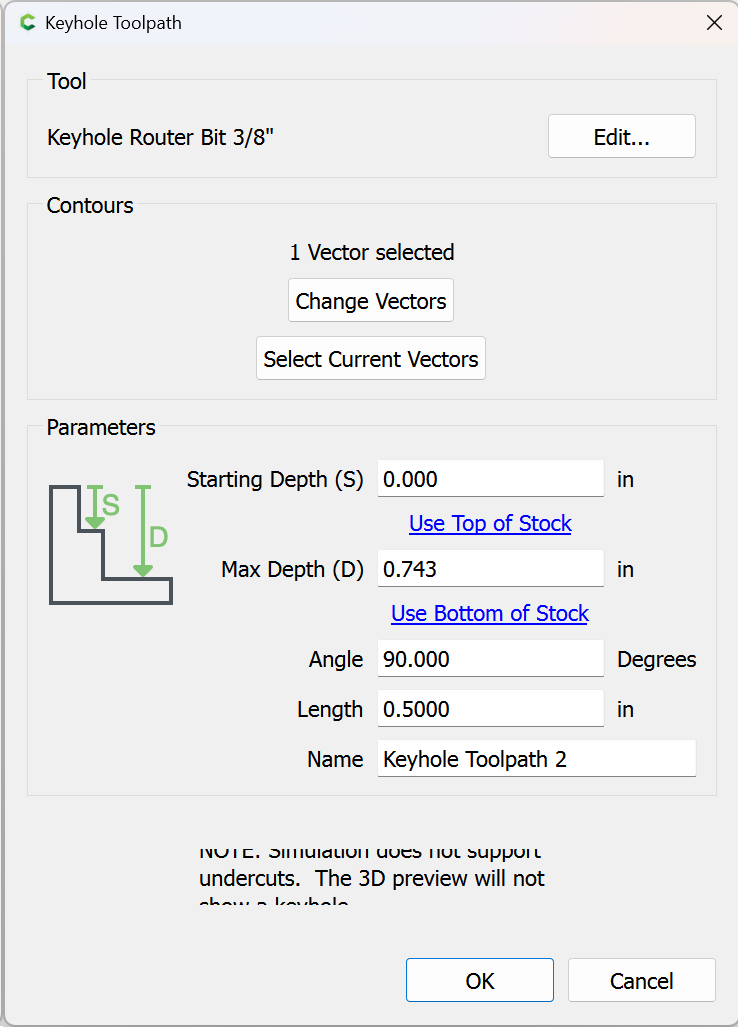
\includegraphics[width=\linewidth/2]{C:/Users/willa/OneDrive/Documents/GitHub/gcodepreview/images/cc8_dialog_toolpath_keyhole.png}\par
\end{centering}

\noindent Hence the parameters:

\begin{itemize}
\item Starting Depth == \verb|kh_start_depth|
\item Max Depth == \verb|kh_max_depth|
\item Angle == \verb|kht_direction|
\item Length == \verb|kh_distance|
\item Tool == \verb|kh_tool_num|
\end{itemize}

Due to the possibility of rotation, for the in-between positions there are more cases than one would think — for each quadrant there are the following possibilities:

\begin{itemize}
 \item one node on the clockwise side is outside of the quadrant
 \item two nodes on the clockwise side are outside of the quadrant
 \item all nodes are w/in the quadrant
 \item one node on the counter-clockwise side is outside of the quadrant
 \item two nodes on the counter-clockwise side are outside of the quadrant
\end{itemize}
 
Supporting all of these would require trigonometric comparisons in the If else blocks, so only the 4 quadrants, N, S, E, and W will be supported in the initial version. This will be done by wrapping the command with a version which only accepts those options: 

\lstset{firstnumber=\thegcpy}
\begin{writecode}{a}{gcodepreview.py}{python}
    def cutkeyholegcdxf(self, kh_start_depth, kh_max_depth, kht_direction, kh_distance, kh_tool_num):   
        if (kht_direction == "N"): 
            toolpath = self.cutKHgcdxf(kh_start_depth, kh_max_depth, 90, kh_distance, kh_tool_num)
            return toolpath
        elif (kht_direction == "S"):
            toolpath = self.cutKHgcdxf(kh_start_depth, kh_max_depth, 270, kh_distance, kh_tool_num)
            return toolpath
        elif (kht_direction == "E"):
            toolpath = self.cutKHgcdxf(kh_start_depth, kh_max_depth, 0, kh_distance, kh_tool_num)
            return toolpath
        elif (kht_direction == "W"):
            toolpath = self.cutKHgcdxf(kh_start_depth, kh_max_depth, 180, kh_distance, kh_tool_num)
            return toolpath

\end{writecode}
\addtocounter{gcpy}{14}
 
The original version of the command, \DescribeRoutine{cutKHgcdxf} retains an interface which allows calling it for arbitrary beginning and ending points of an arc. Note that code is still present for the partial calculation of one quadrant (for the case of all nodes within the quadrant).

The first task is to place a circle at the origin which is invariant of angle:
 
\lstset{firstnumber=\thegcpy}
\begin{writecode}{a}{gcodepreview.py}{python}
    def cutKHgcdxf(self, kh_start_depth, kh_max_depth, kh_angle, kh_distance, kh_tool_num):
        oXpos = self.xpos()
        oYpos = self.ypos()
#Circle at entry hole
#    def dxfarc(self, xcenter, ycenter, radius, anglebegin, endangle, tn):
#        print(self.tool_radius(kh_tool_num, 7))
        self.dxfarc(kh_tool_num, self.xpos(),self.ypos(),self.tool_radius(kh_tool_num, 7),  0, 90)
        self.dxfarc(kh_tool_num, self.xpos(),self.ypos(),self.tool_radius(kh_tool_num, 7), 90,180)
        self.dxfarc(kh_tool_num, self.xpos(),self.ypos(),self.tool_radius(kh_tool_num, 7),180,270)
        self.dxfarc(kh_tool_num, self.xpos(),self.ypos(),self.tool_radius(kh_tool_num, 7),270,360)
        toolpath = self.cutline(self.xpos(), self.ypos(), -kh_max_depth)

\end{writecode}
\addtocounter{gcpy}{12}

Then it will be necessary to test for each possible case in a series of If Else blocks:
 
\lstset{firstnumber=\thegcpy}
\begin{writecode}{a}{gcodepreview.py}{python}
#pre-calculate needed values
        r = self.tool_radius(kh_tool_num, 7)
#        print(r)
        rt = self.tool_radius(kh_tool_num, 1)
#        print(rt)
        ro = math.sqrt((self.tool_radius(kh_tool_num, 1))**2-(self.tool_radius(kh_tool_num, 7))**2)
#        print(ro)
        angle = math.degrees(math.acos(ro/rt))
#Outlines of entry hole and slot
        if (kh_angle == 0):
#Lower left of entry hole
            self.dxfarc(kh_tool_num, self.xpos(),self.ypos(),self.tool_radius(kh_tool_num, 1),180,270)
#Upper left of entry hole
            self.dxfarc(kh_tool_num, self.xpos(),self.ypos(),self.tool_radius(kh_tool_num, 1),90,180)
#Upper right of entry hole
#            self.dxfarc(kh_tool_num, self.xpos(), self.ypos(), rt, 41.810, 90)
            self.dxfarc(kh_tool_num, self.xpos(), self.ypos(), rt, angle, 90)
#Lower right of entry hole
            self.dxfarc(kh_tool_num, self.xpos(), self.ypos(), rt, 270, 360-angle)
#            self.dxfarc(kh_tool_num, self.xpos(),self.ypos(),self.tool_radius(kh_tool_num, 1),270, 270+math.acos(math.radians(self.tool_diameter(kh_tool_num, 5)/self.tool_diameter(kh_tool_num, 1))))
#Actual line of cut
#            self.dxfline(kh_tool_num, self.xpos(),self.ypos(),self.xpos()+kh_distance,self.ypos())
#upper right of end of slot (kh_max_depth+4.36))/2
            self.dxfarc(kh_tool_num, self.xpos()+kh_distance,self.ypos(),self.tool_diameter(kh_tool_num, (kh_max_depth+4.36))/2,0,90)
#lower right of end of slot
            self.dxfarc(kh_tool_num, self.xpos()+kh_distance,self.ypos(),self.tool_diameter(kh_tool_num, (kh_max_depth+4.36))/2,270,360)
#upper right slot
            self.dxfline(kh_tool_num, self.xpos()+ro, self.ypos()-(self.tool_diameter(kh_tool_num,7)/2), self.xpos()+kh_distance, self.ypos()-(self.tool_diameter(kh_tool_num,7)/2))
#            self.dxfline(kh_tool_num, self.xpos()+(sqrt((self.tool_diameter(kh_tool_num,1)^2)-(self.tool_diameter(kh_tool_num,5)^2))/2), self.ypos()+self.tool_diameter(kh_tool_num, (kh_max_depth))/2, ( (kh_max_depth-6.34))/2)^2-(self.tool_diameter(kh_tool_num, (kh_max_depth-6.34))/2)^2, self.xpos()+kh_distance, self.ypos()+self.tool_diameter(kh_tool_num, (kh_max_depth))/2, kh_tool_num)
#end position at top of slot
#lower right slot
            self.dxfline(kh_tool_num, self.xpos()+ro, self.ypos()+(self.tool_diameter(kh_tool_num,7)/2), self.xpos()+kh_distance, self.ypos()+(self.tool_diameter(kh_tool_num,7)/2))
#        dxfline(kh_tool_num, self.xpos()+(sqrt((self.tool_diameter(kh_tool_num,1)^2)-(self.tool_diameter(kh_tool_num,5)^2))/2), self.ypos()-self.tool_diameter(kh_tool_num, (kh_max_depth))/2, ( (kh_max_depth-6.34))/2)^2-(self.tool_diameter(kh_tool_num, (kh_max_depth-6.34))/2)^2, self.xpos()+kh_distance, self.ypos()-self.tool_diameter(kh_tool_num, (kh_max_depth))/2, KH_tool_num)
#end position at top of slot
#    hull(){
#      translate([xpos(), ypos(), zpos()]){
#        gcp_keyhole_shaft(6.35, 9.525);
#      }
#      translate([xpos(), ypos(), zpos()-kh_max_depth]){
#        gcp_keyhole_shaft(6.35, 9.525);
#      }
#    }
#    hull(){
#      translate([xpos(), ypos(), zpos()-kh_max_depth]){
#        gcp_keyhole_shaft(6.35, 9.525);
#      }
#      translate([xpos()+kh_distance, ypos(), zpos()-kh_max_depth]){
#        gcp_keyhole_shaft(6.35, 9.525);
#      }
#    }
#    cutwithfeed(getxpos(),getypos(),-kh_max_depth,feed);
#    cutwithfeed(getxpos()+kh_distance,getypos(),-kh_max_depth,feed);
#    setxpos(getxpos()-kh_distance);
#  } else if (kh_angle > 0 && kh_angle < 90) {
#//echo(kh_angle);
#  dxfarc(getxpos(),getypos(),tool_diameter(KH_tool_num, (kh_max_depth))/2,90+kh_angle,180+kh_angle, KH_tool_num);
#  dxfarc(getxpos(),getypos(),tool_diameter(KH_tool_num, (kh_max_depth))/2,180+kh_angle,270+kh_angle, KH_tool_num);
#dxfarc(getxpos(),getypos(),tool_diameter(KH_tool_num, (kh_max_depth))/2,kh_angle+asin((tool_diameter(KH_tool_num, (kh_max_depth+4.36))/2)/(tool_diameter(KH_tool_num, (kh_max_depth))/2)),90+kh_angle, KH_tool_num);
#dxfarc(getxpos(),getypos(),tool_diameter(KH_tool_num, (kh_max_depth))/2,270+kh_angle,360+kh_angle-asin((tool_diameter(KH_tool_num, (kh_max_depth+4.36))/2)/(tool_diameter(KH_tool_num, (kh_max_depth))/2)), KH_tool_num);
#dxfarc(getxpos()+(kh_distance*cos(kh_angle)),
#  getypos()+(kh_distance*sin(kh_angle)),tool_diameter(KH_tool_num, (kh_max_depth+4.36))/2,0+kh_angle,90+kh_angle, KH_tool_num);
#dxfarc(getxpos()+(kh_distance*cos(kh_angle)),getypos()+(kh_distance*sin(kh_angle)),tool_diameter(KH_tool_num, (kh_max_depth+4.36))/2,270+kh_angle,360+kh_angle, KH_tool_num);
#dxfline( getxpos()+tool_diameter(KH_tool_num, (kh_max_depth))/2*cos(kh_angle+asin((tool_diameter(KH_tool_num, (kh_max_depth+4.36))/2)/(tool_diameter(KH_tool_num, (kh_max_depth))/2))),
# getypos()+tool_diameter(KH_tool_num, (kh_max_depth))/2*sin(kh_angle+asin((tool_diameter(KH_tool_num, (kh_max_depth+4.36))/2)/(tool_diameter(KH_tool_num, (kh_max_depth))/2))),
# getxpos()+(kh_distance*cos(kh_angle))-((tool_diameter(KH_tool_num, (kh_max_depth+4.36))/2)*sin(kh_angle)),
# getypos()+(kh_distance*sin(kh_angle))+((tool_diameter(KH_tool_num, (kh_max_depth+4.36))/2)*cos(kh_angle)), KH_tool_num);
#//echo("a",tool_diameter(KH_tool_num, (kh_max_depth+4.36))/2);
#//echo("c",tool_diameter(KH_tool_num, (kh_max_depth))/2);
#echo("Aangle",asin((tool_diameter(KH_tool_num, (kh_max_depth+4.36))/2)/(tool_diameter(KH_tool_num, (kh_max_depth))/2)));
#//echo(kh_angle);
# cutwithfeed(getxpos()+(kh_distance*cos(kh_angle)),getypos()+(kh_distance*sin(kh_angle)),-kh_max_depth,feed);
            toolpath = toolpath.union(self.cutline(self.xpos()+kh_distance, self.ypos(), -kh_max_depth))
        elif (kh_angle == 90):
#Lower left of entry hole
            self.dxfarc(kh_tool_num, self.xpos(),self.ypos(),self.tool_radius(kh_tool_num, 1),180,270)
#Lower right of entry hole
            self.dxfarc(kh_tool_num, self.xpos(),self.ypos(),self.tool_radius(kh_tool_num, 1),270,360)
#left slot
            self.dxfline(kh_tool_num, self.xpos()-r, self.ypos()+ro, self.xpos()-r, self.ypos()+kh_distance)
#right slot
            self.dxfline(kh_tool_num, self.xpos()+r, self.ypos()+ro, self.xpos()+r, self.ypos()+kh_distance)
#upper left of end of slot
            self.dxfarc(kh_tool_num, self.xpos(),self.ypos()+kh_distance,r,90,180)
#upper right of end of slot
            self.dxfarc(kh_tool_num, self.xpos(),self.ypos()+kh_distance,r,0,90)
#Upper right of entry hole
            self.dxfarc(kh_tool_num, self.xpos(), self.ypos(), rt, 0, 90-angle)
#Upper left of entry hole
            self.dxfarc(kh_tool_num, self.xpos(), self.ypos(), rt, 90+angle, 180)
            toolpath = toolpath.union(self.cutline(self.xpos(), self.ypos()+kh_distance, -kh_max_depth))
        elif (kh_angle == 180):
#Lower right of entry hole
            self.dxfarc(kh_tool_num, self.xpos(),self.ypos(),self.tool_radius(kh_tool_num, 1),270,360)
#Upper right of entry hole
            self.dxfarc(kh_tool_num, self.xpos(),self.ypos(),self.tool_radius(kh_tool_num, 1),0,90)
#Upper left of entry hole
            self.dxfarc(kh_tool_num, self.xpos(), self.ypos(), rt, 90, 180-angle)
#Lower left of entry hole
            self.dxfarc(kh_tool_num, self.xpos(), self.ypos(), rt, 180+angle, 270)
#upper slot
            self.dxfline(kh_tool_num, self.xpos()-ro, self.ypos()-r, self.xpos()-kh_distance, self.ypos()-r)
#lower slot
            self.dxfline(kh_tool_num, self.xpos()-ro, self.ypos()+r, self.xpos()-kh_distance, self.ypos()+r)
#upper left of end of slot
            self.dxfarc(kh_tool_num, self.xpos()-kh_distance,self.ypos(),r,90,180)
#lower left of end of slot
            self.dxfarc(kh_tool_num, self.xpos()-kh_distance,self.ypos(),r,180,270)
            toolpath = toolpath.union(self.cutline(self.xpos()-kh_distance, self.ypos(), -kh_max_depth))
        elif (kh_angle == 270):
#Upper left of entry hole
            self.dxfarc(kh_tool_num, self.xpos(),self.ypos(),self.tool_radius(kh_tool_num, 1),90,180)
#Upper right of entry hole
            self.dxfarc(kh_tool_num, self.xpos(),self.ypos(),self.tool_radius(kh_tool_num, 1),0,90)
#left slot
            self.dxfline(kh_tool_num, self.xpos()-r, self.ypos()-ro, self.xpos()-r, self.ypos()-kh_distance)
#right slot
            self.dxfline(kh_tool_num, self.xpos()+r, self.ypos()-ro, self.xpos()+r, self.ypos()-kh_distance)
#lower left of end of slot
            self.dxfarc(kh_tool_num, self.xpos(),self.ypos()-kh_distance,r,180,270)
#lower right of end of slot
            self.dxfarc(kh_tool_num, self.xpos(),self.ypos()-kh_distance,r,270,360)
#lower right of entry hole
            self.dxfarc(kh_tool_num, self.xpos(), self.ypos(), rt, 180, 270-angle)
#lower left of entry hole
            self.dxfarc(kh_tool_num, self.xpos(), self.ypos(), rt, 270+angle, 360)
            toolpath = toolpath.union(self.cutline(self.xpos(), self.ypos()-kh_distance, -kh_max_depth))
#        print(self.zpos())
        self.setxpos(oXpos)
        self.setypos(oYpos)
        return toolpath
            
#  } else if (kh_angle == 90) {
#    //Lower left of entry hole
#    dxfarc(getxpos(),getypos(),9.525/2,180,270, KH_tool_num);
#    //Lower right of entry hole
#    dxfarc(getxpos(),getypos(),9.525/2,270,360, KH_tool_num);
#    //Upper right of entry hole
#    dxfarc(getxpos(),getypos(),9.525/2,0,acos(tool_diameter(KH_tool_num, 5)/tool_diameter(KH_tool_num, 1)), KH_tool_num);
#    //Upper left of entry hole
#    dxfarc(getxpos(),getypos(),9.525/2,180-acos(tool_diameter(KH_tool_num, 5)/tool_diameter(KH_tool_num, 1)), 180,KH_tool_num);
#    //Actual line of cut
#    dxfline(getxpos(),getypos(),getxpos(),getypos()+kh_distance);
#    //upper right of slot
#    dxfarc(getxpos(),getypos()+kh_distance,tool_diameter(KH_tool_num, (kh_max_depth+4.36))/2,0,90, KH_tool_num);
#    //upper left of slot
#    dxfarc(getxpos(),getypos()+kh_distance,tool_diameter(KH_tool_num, (kh_max_depth+6.35))/2,90,180, KH_tool_num);
#    //right of slot
#    dxfline(
#        getxpos()+tool_diameter(KH_tool_num, (kh_max_depth))/2, 
#        getypos()+(sqrt((tool_diameter(KH_tool_num,1)^2)-(tool_diameter(KH_tool_num,5)^2))/2),//( (kh_max_depth-6.34))/2)^2-(tool_diameter(KH_tool_num, (kh_max_depth-6.34))/2)^2,
#        getxpos()+tool_diameter(KH_tool_num, (kh_max_depth))/2,
#    //end position at top of slot
#        getypos()+kh_distance, 
#        KH_tool_num);
#    dxfline(getxpos()-tool_diameter(KH_tool_num, (kh_max_depth))/2, getypos()+(sqrt((tool_diameter(KH_tool_num,1)^2)-(tool_diameter(KH_tool_num,5)^2))/2), getxpos()-tool_diameter(KH_tool_num, (kh_max_depth+6.35))/2,getypos()+kh_distance, KH_tool_num);
#    hull(){
#      translate([xpos(), ypos(), zpos()]){
#        gcp_keyhole_shaft(6.35, 9.525);
#      }
#      translate([xpos(), ypos(), zpos()-kh_max_depth]){
#        gcp_keyhole_shaft(6.35, 9.525);
#      }
#    }
#    hull(){
#      translate([xpos(), ypos(), zpos()-kh_max_depth]){
#        gcp_keyhole_shaft(6.35, 9.525);
#      }
#      translate([xpos(), ypos()+kh_distance, zpos()-kh_max_depth]){
#        gcp_keyhole_shaft(6.35, 9.525);
#      }
#    }
#    cutwithfeed(getxpos(),getypos(),-kh_max_depth,feed);
#    cutwithfeed(getxpos(),getypos()+kh_distance,-kh_max_depth,feed);
#    setypos(getypos()-kh_distance);
#  } else if (kh_angle == 180) {
#    //Lower right of entry hole
#    dxfarc(getxpos(),getypos(),9.525/2,270,360, KH_tool_num);
#    //Upper right of entry hole
#    dxfarc(getxpos(),getypos(),9.525/2,0,90, KH_tool_num);
#    //Upper left of entry hole
#    dxfarc(getxpos(),getypos(),9.525/2,90, 90+acos(tool_diameter(KH_tool_num, 5)/tool_diameter(KH_tool_num, 1)), KH_tool_num);
#    //Lower left of entry hole
#    dxfarc(getxpos(),getypos(),9.525/2, 270-acos(tool_diameter(KH_tool_num, 5)/tool_diameter(KH_tool_num, 1)), 270, KH_tool_num);
#    //upper left of slot
#    dxfarc(getxpos()-kh_distance,getypos(),tool_diameter(KH_tool_num, (kh_max_depth+6.35))/2,90,180, KH_tool_num);
#    //lower left of slot
#    dxfarc(getxpos()-kh_distance,getypos(),tool_diameter(KH_tool_num, (kh_max_depth+6.35))/2,180,270, KH_tool_num);
#    //Actual line of cut
#    dxfline(getxpos(),getypos(),getxpos()-kh_distance,getypos());
#    //upper left slot
#    dxfline(
#        getxpos()-(sqrt((tool_diameter(KH_tool_num,1)^2)-(tool_diameter(KH_tool_num,5)^2))/2), 
#        getypos()+tool_diameter(KH_tool_num, (kh_max_depth))/2,//( (kh_max_depth-6.34))/2)^2-(tool_diameter(KH_tool_num, (kh_max_depth-6.34))/2)^2,
#        getxpos()-kh_distance,
#    //end position at top of slot
#        getypos()+tool_diameter(KH_tool_num, (kh_max_depth))/2, 
#        KH_tool_num);
#    //lower right slot
#    dxfline(
#        getxpos()-(sqrt((tool_diameter(KH_tool_num,1)^2)-(tool_diameter(KH_tool_num,5)^2))/2), 
#        getypos()-tool_diameter(KH_tool_num, (kh_max_depth))/2,//( (kh_max_depth-6.34))/2)^2-(tool_diameter(KH_tool_num, (kh_max_depth-6.34))/2)^2,
#        getxpos()-kh_distance,
#    //end position at top of slot
#        getypos()-tool_diameter(KH_tool_num, (kh_max_depth))/2, 
#        KH_tool_num);
#    hull(){
#      translate([xpos(), ypos(), zpos()]){
#        gcp_keyhole_shaft(6.35, 9.525);
#      }
#      translate([xpos(), ypos(), zpos()-kh_max_depth]){
#        gcp_keyhole_shaft(6.35, 9.525);
#      }
#    }
#    hull(){
#      translate([xpos(), ypos(), zpos()-kh_max_depth]){
#        gcp_keyhole_shaft(6.35, 9.525);
#      }
#      translate([xpos()-kh_distance, ypos(), zpos()-kh_max_depth]){
#        gcp_keyhole_shaft(6.35, 9.525);
#      }
#    }
#    cutwithfeed(getxpos(),getypos(),-kh_max_depth,feed);
#    cutwithfeed(getxpos()-kh_distance,getypos(),-kh_max_depth,feed);
#    setxpos(getxpos()+kh_distance);
#  } else if (kh_angle == 270) {
#    //Upper right of entry hole
#    dxfarc(getxpos(),getypos(),9.525/2,0,90, KH_tool_num);
#    //Upper left of entry hole
#    dxfarc(getxpos(),getypos(),9.525/2,90,180, KH_tool_num);
#    //lower right of slot
#    dxfarc(getxpos(),getypos()-kh_distance,tool_diameter(KH_tool_num, (kh_max_depth+4.36))/2,270,360, KH_tool_num);
#    //lower left of slot
#    dxfarc(getxpos(),getypos()-kh_distance,tool_diameter(KH_tool_num, (kh_max_depth+4.36))/2,180,270, KH_tool_num);
#    //Actual line of cut
#    dxfline(getxpos(),getypos(),getxpos(),getypos()-kh_distance);
#    //right of slot
#    dxfline(
#        getxpos()+tool_diameter(KH_tool_num, (kh_max_depth))/2, 
#        getypos()-(sqrt((tool_diameter(KH_tool_num,1)^2)-(tool_diameter(KH_tool_num,5)^2))/2),//( (kh_max_depth-6.34))/2)^2-(tool_diameter(KH_tool_num, (kh_max_depth-6.34))/2)^2,
#        getxpos()+tool_diameter(KH_tool_num, (kh_max_depth))/2,
#    //end position at top of slot
#        getypos()-kh_distance, 
#        KH_tool_num);
#    //left of slot
#    dxfline(
#        getxpos()-tool_diameter(KH_tool_num, (kh_max_depth))/2, 
#        getypos()-(sqrt((tool_diameter(KH_tool_num,1)^2)-(tool_diameter(KH_tool_num,5)^2))/2),//( (kh_max_depth-6.34))/2)^2-(tool_diameter(KH_tool_num, (kh_max_depth-6.34))/2)^2,
#        getxpos()-tool_diameter(KH_tool_num, (kh_max_depth))/2,
#    //end position at top of slot
#        getypos()-kh_distance, 
#        KH_tool_num);
#    //Lower right of entry hole
#    dxfarc(getxpos(),getypos(),9.525/2,360-acos(tool_diameter(KH_tool_num, 5)/tool_diameter(KH_tool_num, 1)), 360, KH_tool_num);
#    //Lower left of entry hole
#    dxfarc(getxpos(),getypos(),9.525/2,180, 180+acos(tool_diameter(KH_tool_num, 5)/tool_diameter(KH_tool_num, 1)), KH_tool_num);
#    hull(){
#      translate([xpos(), ypos(), zpos()]){
#        gcp_keyhole_shaft(6.35, 9.525);
#      }
#      translate([xpos(), ypos(), zpos()-kh_max_depth]){
#        gcp_keyhole_shaft(6.35, 9.525);
#      }
#    }
#    hull(){
#      translate([xpos(), ypos(), zpos()-kh_max_depth]){
#        gcp_keyhole_shaft(6.35, 9.525);
#      }
#      translate([xpos(), ypos()-kh_distance, zpos()-kh_max_depth]){
#        gcp_keyhole_shaft(6.35, 9.525);
#      }
#    }
#    cutwithfeed(getxpos(),getypos(),-kh_max_depth,feed);
#    cutwithfeed(getxpos(),getypos()-kh_distance,-kh_max_depth,feed);
#    setypos(getypos()+kh_distance);
#  }
#}

\end{writecode}
\addtocounter{gcpy}{107}

Lastly, to use the class it will be necessary to load it:

\lstset{firstnumber=\thegcpy}
\begin{writecode}{a}{gcodepreview.py}{python}
from gcodepreview import *

\end{writecode}
\addtocounter{gcpy}{2}

\noindent which may then allow loading the the class as expected. \url{https://github.com/gsohler/openscad/issues/48}
 
\subsection{Shapes and tool movement}
 
The majority of commands will be more general, focusing on tooling which is generally supported by this library, moving in lines and arcs so as to describe shapes which lend themselves to representation with those tool and which match up with both toolpaths and supported geometry in Carbide Create, and the usage requirements of the typical user.

\subsubsection{Generalized commands and cuts}

The first consideration is a naming convention which will allow a generalized set of associated commands to be defined. The initial version will only create OpenSCAD commands for 3D modeling and write out matching DXF files. At a later time this will be extended with G-code support.
 
\paragraph{begincutdxf}
 
The first command, \DescribeRoutine{begincutdxf} will need to allow the machine to rapid to the beginning point of the cut and then rapid down to the surface of the stock, and then plunge down to the depth of the cut. The implementation will need to allow for a hook where the Depth per Pass is applied to the plunge operation so that multiple passes are made.

The first module will ensure that the tool is safely up above the stock and will rapid to the position specified at the retract height (moving to that position as an initial step, then will \texttt{cutwithfeed} to the specified position at the specified feed rate. Despite \texttt{dxf} being included in the filename no change is made to the dxf file at this time, this simply indicates that this file is preparatory to the use of \DescribeRoutine{continuecutdxf}.

\lstset{firstnumber=\thegcpscad}
\begin{writecode}{a}{gcodepreview.scad}{scad}
module begincutdxf(rh, ex, ey, ez, fr) {
  rapid(getxpos(),getypos(),rh);
  cutwithfeed(ex,ey,ez,fr);
}

\end{writecode}
\addtocounter{gcpscad}{5}
 
\lstset{firstnumber=\thegcpscad}
\begin{writecode}{a}{gcodepreview.scad}{scad}
module continuecutdxf(ex, ey, ez, fr) {
  cutwithfeed(ex,ey,ez,fr);
}

\end{writecode}
\addtocounter{gcpscad}{4}

\paragraph{Rectangles}

Cutting rectangles while writing out their perimeter in the DXF files (so that they may be assigned a matching toolpath in a traditional CAM program upon import) will require the origin coordinates, height and width and depth of the pocket, and the tool \# so that the corners may have a radius equal to the tool which is used. Whether a given module is an interior pocket or an outline (interior or exterior) will be determined by the specifics of the module and its usage/positioning, with \texttt{outline} being added to those modules which cut perimeter.

A further consideration is that cut orientation as an option should be accounted for if writing out G-code, as well as stepover, and the nature of initial entry (whether ramping in would be implemented, and if so, at what angle). Advanced toolpath strategies such as trochoidal milling could also be implemented.

Th routine \DescribeRoutine{cutrectangledxf} cuts the outline of a rectangle creating sharp corners. Note that the initial version would work as a beginning point for vertical cutting if the \texttt{hull()} operation was removed and the loop was uncommented:
 
\lstset{firstnumber=\thegcpscad}
\begin{writecode}{a}{gcodepreview.scad}{scad}
module cutrectangledxf(bx, by, bz, rwidth, rheight, rdepth, rtn) {//passes
  movetosafez();
  hull(){
    //  for (i = [0 : abs(1) : passes]) {
    //      rapid(bx+tool_radius(rtn)+i*(rwidth-tool_diameter(current_tool()))/passes,bx+tool_radius(rtn),1);
    //      cutwithfeed(bx+tool_radius(rtn)+i*(rwidth-tool_diameter(current_tool()))/passes,by+tool_radius(rtn),bz-rdepth,feed);
    //      cutwithfeed(bx+tool_radius(rtn)+i*(rwidth-tool_diameter(current_tool()))/passes,by+rheight-tool_radius(rtn),bz-rdepth,feed);
  
    cutwithfeed(bx+tool_radius(rtn),by+tool_radius(rtn),bz-rdepth,feed);
    cutwithfeed(bx+rwidth-tool_radius(rtn),by+tool_radius(rtn),bz-rdepth,feed);
    cutwithfeed(bx+rwidth-tool_radius(rtn),by+rheight-tool_radius(rtn),bz-rdepth,feed);
    cutwithfeed(bx+tool_radius(rtn),by+rheight-tool_radius(rtn),bz-rdepth,feed);
  }
  //dxfarc(xcenter,ycenter,radius,anglebegin,endangle, tn)
  dxfarc(bx+tool_radius(rtn),by+tool_radius(rtn),tool_radius(rtn),180,270, rtn);
  //dxfline(xbegin,ybegin,xend,yend, tn)
  dxfline(bx,by+tool_radius(rtn),bx,by+rheight-tool_radius(rtn), rtn);
  dxfarc(bx+tool_radius(rtn),by+rheight-tool_radius(rtn),tool_radius(rtn),90,180, rtn);
  dxfline(bx+tool_radius(rtn),by+rheight,bx+rwidth-tool_radius(rtn),by+rheight, rtn);
  dxfarc(bx+rwidth-tool_radius(rtn),by+rheight-tool_radius(rtn),tool_radius(rtn),0,90, rtn);
  dxfline(bx+rwidth,by+rheight-tool_radius(rtn),bx+rwidth,by+tool_radius(rtn), rtn);
  dxfarc(bx+rwidth-tool_radius(rtn),by+tool_radius(rtn),tool_radius(rtn),270,360, rtn);
  dxfline(bx+rwidth-tool_radius(rtn),by,bx+tool_radius(rtn),by, rtn);
}

\end{writecode}
\addtocounter{gcpscad}{25}

A matching command: \DescribeRoutine{cutrectangleoutlinedxf} cuts the outline of a rounded rectangle and is a simplification of the above:

\lstset{firstnumber=\thegcpscad}
\begin{writecode}{a}{gcodepreview.scad}{scad}
module cutrectangleoutlinedxf(bx, by, bz, rwidth, rheight, rdepth, rtn) {//passes
  movetosafez();
  cutwithfeed(bx+tool_radius(rtn),by+tool_radius(rtn),bz-rdepth,feed);
  cutwithfeed(bx+rwidth-tool_radius(rtn),by+tool_radius(rtn),bz-rdepth,feed);
  cutwithfeed(bx+rwidth-tool_radius(rtn),by+rheight-tool_radius(rtn),bz-rdepth,feed);
  cutwithfeed(bx+tool_radius(rtn),by+rheight-tool_radius(rtn),bz-rdepth,feed);
  dxfarc(bx+tool_radius(rtn),by+tool_radius(rtn),tool_radius(rtn),180,270, rtn);
  dxfline(bx,by+tool_radius(rtn),bx,by+rheight-tool_radius(rtn), rtn);
  dxfarc(bx+tool_radius(rtn),by+rheight-tool_radius(rtn),tool_radius(rtn),90,180, rtn);
  dxfline(bx+tool_radius(rtn),by+rheight,bx+rwidth-tool_radius(rtn),by+rheight, rtn);
  dxfarc(bx+rwidth-tool_radius(rtn),by+rheight-tool_radius(rtn),tool_radius(rtn),0,90, rtn);
  dxfline(bx+rwidth,by+rheight-tool_radius(rtn),bx+rwidth,by+tool_radius(rtn), rtn);
  dxfarc(bx+rwidth-tool_radius(rtn),by+tool_radius(rtn),tool_radius(rtn),270,360, rtn);
  dxfline(bx+rwidth-tool_radius(rtn),by,bx+tool_radius(rtn),by, rtn);
}

\end{writecode}
\addtocounter{gcpscad}{16}

Which suggests a further command, \DescribeRoutine{rectangleoutlinedxf} for simply adding a rectangle (a potential use of which would be in Job Setup to add the stock outline to \textsc{dxf}s to assist in registration of jobs with multiple tools):

\lstset{firstnumber=\thegcpscad}
\begin{writecode}{a}{gcodepreview.scad}{scad}
module rectangleoutlinedxf(bx, by, bz, rwidth, rheight, rtn) {
  dxfline(bx,by,bx,by+rheight, rtn);
  dxfline(bx,by+rheight,bx+rwidth,by+rheight, rtn);
  dxfline(bx+rwidth,by+rheight,bx+rwidth,by, rtn);
  dxfline(bx+rwidth,by,bx,by, rtn);
}

\end{writecode}
\addtocounter{gcpscad}{7}

\noindent the initial section performs the cutting operation for the 3D preview while the latter section writes out the outline to the DXF files.

A variant of the  cutting version of that file, \DescribeRoutine{cutoutrectangledxf} will cut to the outside:

\lstset{firstnumber=\thegcpscad}
\begin{writecode}{a}{gcodepreview.scad}{scad}
module cutoutrectangledxf(bx, by, bz, rwidth, rheight, rdepth, rtn) {
  movetosafez();
  cutwithfeed(bx-tool_radius(rtn),by-tool_radius(rtn),bz-rdepth,feed);
  cutwithfeed(bx+rwidth+tool_radius(rtn),by-tool_radius(rtn),bz-rdepth,feed);
  cutwithfeed(bx+rwidth+tool_radius(rtn),by+rheight+tool_radius(rtn),bz-rdepth,feed);
  cutwithfeed(bx-tool_radius(rtn),by+rheight+tool_radius(rtn),bz-rdepth,feed);
  cutwithfeed(bx-tool_radius(rtn),by-tool_radius(rtn),bz-rdepth,feed);
  dxfline(bx,by,bx,by+rheight, rtn);
  dxfline(bx,by+rheight,bx+rwidth,by+rheight, rtn);
  dxfline(bx+rwidth,by+rheight,bx+rwidth,by, rtn);
  dxfline(bx+rwidth,by,bx,by, rtn);
}

\end{writecode}
\addtocounter{gcpscad}{13}

%\subsection{Expansion}
%
%The balance of shapes will go into \texttt{cut2Dshapes.scad} and of course it will be possible to create additional files for specific purposes.
%
%\lstset{firstnumber=1}
%\begin{writecode}{w}{cut2Dshapes.scad}{scad}
%//!OpenSCAD
%
%\end{writecode}
%\addtocounter{cuttwod}{2}

\section{Future}

\subsection*{Images}

Would it be helpful to re-create code algorithms/sections using OpenSCAD Graph Editor so as to represent/illustrate the program?

%\subsection{Generalized DXF creation}
%
%Generalize the creation of DXFs based on the projection() of a toolpath?

\subsection*{Import G-code}

Use a tool to read in a G-code file, then create a 3D model which would serve as a preview of the cut?

\begin{itemize}
\item \url{https://stackoverflow.com/questions/34638372/simple-python-program-to-read-gcode-file}
\item \url{https://pypi.org/project/gcodeparser/}
\item \url{https://github.com/fragmuffin/pygcode/wiki}
\end{itemize} 
 
\subsection*{Bézier curves in 2 dimensions}

Take a Bézier curve definition and approximate it as arcs and write them into a DXF?

\url{https://pomax.github.io/bezierinfo/}

c.f., \url{https://linuxcnc.org/docs/html/gcode/g-code.html#gcode:g5}

%There is Bernstein polynomial equation which is similar to calculating like $(a+b)^2 ....$ or up to $(a+b)^n$ where $n$ is the degree of polynomial.
%
%So how do you calculate $(a+b)^2$ or for that matter to any polynomial degree $n$
%
%an integer $i => 0 to n$ calculates each term of the above equation
%
%$n!/(i! * (n-i)!)*a^i*b^(n-i)$  where $n!$ means factorial of $n$ --equation 1
%substituting $a=t$ and $b=(1-t)$
%where $t$ is a parameter which goes from $0 ->1$ and you can have any numbers within that range
%
%in bezier the degree of the curve is 1 less than the control points e.g. if you have 10 control points the polynomial degree will be 9.
%
%so finally equation for bezier is:
%
%$sum(p[i]*n!/(i! * (n-i)!)*t^i*(1-t)^(n-i))$ where $p[i]$ is the $i$th control point
%
%my simple 6 lines function for bezier curve is following:
%
%\begin{verbatim}
%def bezier(p,s=10):
%  r  '''
%    bezier curve defined by points 'p' and number of segments 's'
%    '''
%    p=a_(p)
%    n=len(p)
%    k=n-1
%    f=[[p[i]*comb(k,i)*u**i*(1-u)**(k-i) for i in range(n)]
%       for u in linspace(0,1,s)]    
%    p1=l_(a_([p.sum(0) for p in a_(f)]))
%    return p1
%\end{verbatim}    

\subsection*{Bézier curves in 3 dimensions}
 
One question is how many Bézier curves would it be necessary to have to define a surface in 3~dimensions. Attributes for this which are desirable/necessary:

\begin{itemize}
\item concise --- a given Bézier curve should be represented by just the point coordinates, 
      so two on-curve points, two off-curve points, each with a pair of coordinates
\item For a given shape/region it will need to be possible to have a matching definition 
      exactly match up with it so that one could piece together a larger more complex shape 
      from smaller/simpler regions
\item similarly it will be necessary for it to be possible to sub-divide a defined region --- 
      for example it should be possible if one had 4 adjacent regions, then the four quadrants 
      at the intersection of the four regions could be used to construct a new region --- is it
      possible to derive a new Bézier curve from half of two other curves?
\end{itemize}

\begin{samepage}
For the three planes:

\begin{itemize}
 \item XY
 \item XZ
 \item ZY
\end{itemize}
 
\noindent it should be possible to have three Bézier curves (left-most/right-most or front-back or top/bottom for two, and a mid-line for the third), so a region which can be so represented would be definable by:
 
\begin{verbatim}
3 planes * 3 Béziers * (2 on-curve + 2 off-curve points) == 36 coordinate pairs
\end{verbatim}
\end{samepage}
 
\noindent which is a marked contrast to representations such as:
 
\url{https://github.com/DavidPhillipOster/Teapot}

\noindent and regions which could not be so represented could be sub-divided until the representation is workable.

Or, it may be that fewer (only two?) curves are needed:

\noindent\includegraphics[width=\linewidth]{images/Screenshot 2024-08-11 at 6.55.26 PM.png}

\url{https://pages.mtu.edu/~shene/COURSES/cs3621/NOTES/notes.html}

c.f., \url{https://github.com/BelfrySCAD/BOSL2/wiki/nurbs.scad} and \url{https://old.reddit.com/r/OpenPythonSCAD/comments/1gjcz4z/pythonscad_will_get_a_new_spline_function/}

\section{Other Resources}
 
Holidays are from \url{https://nationaltoday.com/}

\subsection*{DXFs}

\url{http://www.paulbourke.net/dataformats/dxf/}

\noindent\url{https://paulbourke.net/dataformats/dxf/min3d.html}


%This document was re-worked per: \url{https://tex.stackexchange.com/questions/47237/different-approach-to-literate-programming-for-latex}
 
%https://www.semanticscholar.org/paper/A-Philosophy-of-Software-Design-Ousterhout/93cf2d44a3e9d94b059a0e4c68b477cfefc5fef9

\bibliographystyle{alpha}

\begin{thebibliography}{Ousterhout2018APO}

\bibitem[ConstGeom]{WALMSLEY81}
Walmsley, Brian. \emph{Construction Geometry}. 2d ed., Centennial College Press, 1981.
 
\bibitem[MkCalc]{HORVATH22}
Horvath, Joan, and Rich Cameron. 
\emph{Make: Calculus: Build models to learn, visualize, and explore}. First edition., 
Make: Community LLC, 2022.
 
\bibitem[MkGeom]{HORVATH21}
Horvath, Joan, and Rich Cameron. 
\emph{Make: Geometry: Learn by 3D Printing, Coding and Exploring}. First edition., 
Make: Community LLC, 2021.

\bibitem[MkTrig]{HORVATH23}
Horvath, Joan, and Rich Cameron. 
\emph{Make: Trigonometry: Build your way from triangles to analytic geometry}. First edition., 
Make: Community LLC, 2023.
 
\bibitem[PractShopMath]{BEGNAL18}
Begnal, Tom. \emph{Practical Shop Math: Simple Solutions to Workshop Fractions, Formulas + Geometric Shapes}. Updated edition, Spring House Press, 2018.
 
\bibitem[RS274]{KRAMER00}
Thomas R. Kramer, Frederick M. Proctor, Elena R. Messina.\\
\mbox{\url{https://tsapps.nist.gov/publication/get_pdf.cfm?pub_id=823374}}\\
\url{https://www.nist.gov/publications/nist-rs274ngc-interpreter-version-3}

\bibitem[SoftwareDesign]{Ousterhout2018APO}
Ousterhout, John K.
\emph{A Philosophy of Software Design}. First Edition., Yaknyam Press, Palo Alto, Ca., 2018

%  title={A Philosophy of Software Design},
%  author={ Ousterhout},
%  year={2018},
%  url={https://api.semanticscholar.org/CorpusID:69749255}


\end{thebibliography}

\createindexes

 
%\MergeAllFiles{readme.md}
%\MergeAllFiles{interfaces.txt}
\MergeAllFiles{gcodepreview.py}
\MergeAllFiles{pygcodepreview.scad}
\MergeAllFiles{gcodepreview.scad}
\MergeAllFiles{gcodepreviewtemplate.scad}
\MergeAllFiles{gcodepreviewtemplate.py}
\MergeAllFiles{gcpdxf.py}
%\MergeAllFiles{cut2Dshapes.scad}

\end{document}

